\documentclass[journal,12pt,twocolumn]{IEEEtran}
%
\usepackage{setspace}
\usepackage{gensymb}
%\doublespacing
\singlespacing

%\usepackage{graphicx}
%\usepackage{amssymb}
%\usepackage{relsize}
\usepackage[cmex10]{amsmath}
%\usepackage{amsthm}
%\interdisplaylinepenalty=2500
%\savesymbol{iint}
%\usepackage{txfonts}
%\restoresymbol{TXF}{iint}
%\usepackage{wasysym}
\usepackage{amsthm}
\usepackage{iithtlc}
\usepackage{mathrsfs}
\usepackage{txfonts}
\usepackage{stfloats}
\usepackage{bm}
\usepackage{cite}
\usepackage{cases}
\usepackage{subfig}
%\usepackage{xtab}
\usepackage{longtable}
\usepackage{multirow}
%\usepackage{algorithm}
%\usepackage{algpseudocode}
\usepackage{booktabs}
\usepackage{enumitem}
\usepackage{mathtools}
\usepackage{tikz}
\usepackage{pgfplots}
\usepackage{circuitikz}
\usepackage{verbatim}
\usepackage{tfrupee}
\usepackage[breaklinks=true]{hyperref}
%\usepackage{stmaryrd}
\usepackage{tkz-euclide} % loads  TikZ and tkz-base
%\usetkzobj{all}
\usetikzlibrary{fit}
\usetikzlibrary{calc,math}
%\pgfdeclarelayer{background}
%\pgfsetlayers{background}
\usepackage{listings}
    \usepackage{color}                                            %%
    \usepackage{array}                                            %%
    \usepackage{longtable}                                        %%
    \usepackage{calc}                                             %%
    \usepackage{multirow}                                         %%
    \usepackage{hhline}                                           %%
    \usepackage{ifthen}                                           %%
  %optionally (for landscape tables embedded in another document): %%
    \usepackage{lscape}     
\usepackage{multicol}
\usepackage{chngcntr}
%\usepackage{enumerate}

%\usepackage{wasysym}
%\newcounter{MYtempeqncnt}
\DeclareMathOperator*{\Res}{Res}
%\renewcommand{\baselinestretch}{2}
\renewcommand\thesection{\arabic{section}}
\renewcommand\thesubsection{\thesection.\arabic{subsection}}
\renewcommand\thesubsubsection{\thesubsection.\arabic{subsubsection}}

\renewcommand\thesectiondis{\arabic{section}}
\renewcommand\thesubsectiondis{\thesectiondis.\arabic{subsection}}
\renewcommand\thesubsubsectiondis{\thesubsectiondis.\arabic{subsubsection}}

% correct bad hyphenation here
\hyphenation{op-tical net-works semi-conduc-tor}
\def\inputGnumericTable{}                                 %%

\lstset{
%language=C,
frame=single, 
breaklines=true,
columns=fullflexible
}
%\lstset{
%language=tex,
%frame=single, 
%breaklines=true
%}

\begin{document}
%


\newtheorem{theorem}{Theorem}[section]
\newtheorem{problem}{Problem}
\newtheorem{proposition}{Proposition}[section]
\newtheorem{lemma}{Lemma}[section]
\newtheorem{corollary}[theorem]{Corollary}
\newtheorem{example}{Example}[section]
\newtheorem{definition}[problem]{Definition}
%\newtheorem{thm}{Theorem}[section] 
%\newtheorem{defn}[thm]{Definition}
%\newtheorem{algorithm}{Algorithm}[section]
%\newtheorem{cor}{Corollary}
\newcommand{\BEQA}{\begin{eqnarray}}
\newcommand{\EEQA}{\end{eqnarray}}
\newcommand{\define}{\stackrel{\triangle}{=}}
\newcommand{\RomanNumeralCaps}[1]
    {\MakeUppercase{\romannumeral #1}}
\bibliographystyle{IEEEtran}
%\bibliographystyle{ieeetr}


\providecommand{\mbf}{\mathbf}
\providecommand{\pr}[1]{\ensuremath{\Pr\left(#1\right)}}
\providecommand{\qfunc}[1]{\ensuremath{Q\left(#1\right)}}
\providecommand{\sbrak}[1]{\ensuremath{{}\left[#1\right]}}
\providecommand{\lsbrak}[1]{\ensuremath{{}\left[#1\right.}}
\providecommand{\rsbrak}[1]{\ensuremath{{}\left.#1\right]}}
\providecommand{\brak}[1]{\ensuremath{\left(#1\right)}}
\providecommand{\lbrak}[1]{\ensuremath{\left(#1\right.}}
\providecommand{\rbrak}[1]{\ensuremath{\left.#1\right)}}
\providecommand{\cbrak}[1]{\ensuremath{\left\{#1\right\}}}
\providecommand{\lcbrak}[1]{\ensuremath{\left\{#1\right.}}
\providecommand{\rcbrak}[1]{\ensuremath{\left.#1\right\}}}
\theoremstyle{remark}
\newtheorem{rem}{Remark}
\newcommand{\sgn}{\mathop{\mathrm{sgn}}}
\providecommand{\abs}[1]{\left\vert#1\right\vert}
\providecommand{\res}[1]{\Res\displaylimits_{#1}} 
\providecommand{\norm}[1]{\left\lVert#1\right\rVert}
%\providecommand{\norm}[1]{\lVert#1\rVert}
\providecommand{\mtx}[1]{\mathbf{#1}}
\providecommand{\mean}[1]{E\left[ #1 \right]}
\providecommand{\fourier}{\overset{\mathcal{F}}{ \rightleftharpoons}}
%\providecommand{\hilbert}{\overset{\mathcal{H}}{ \rightleftharpoons}}
\providecommand{\system}{\overset{\mathcal{H}}{ \longleftrightarrow}}
	%\newcommand{\solution}[2]{\textbf{Solution:}{#1}}
\newcommand{\solution}{\noindent \textbf{Solution: }}
\newcommand{\cosec}{\,\text{cosec}\,}
\providecommand{\dec}[2]{\ensuremath{\overset{#1}{\underset{#2}{\gtrless}}}}
\newcommand{\myvec}[1]{\ensuremath{\begin{pmatrix}#1\end{pmatrix}}}
\newcommand{\mydet}[1]{\ensuremath{\begin{vmatrix}#1\end{vmatrix}}}
\newcommand*{\permcomb}[4][0mu]{{{}^{#3}\mkern#1#2_{#4}}}
\newcommand*{\perm}[1][-3mu]{\permcomb[#1]{P}}
\newcommand*{\comb}[1][-1mu]{\permcomb[#1]{C}}

%\newcommand*{\perm}[2]{{}^{#1}\!P_{#2}}%
%\newcommand*{\comb}[2]{{}^{#1}C_{#2}}%
%\numberwithin{equation}{section}
\numberwithin{equation}{subsection}
%\numberwithin{problem}{section}
%\numberwithin{definition}{section}
\makeatletter
\@addtoreset{figure}{problem}
\makeatother

\let\StandardTheFigure\thefigure
\let\vec\mathbf
%\renewcommand{\thefigure}{\theproblem.\arabic{figure}}
\renewcommand{\thefigure}{\theproblem}
%\setlist[enumerate,1]{before=\renewcommand\theequation{\theenumi.\arabic{equation}}
%\counterwithin{equation}{enumi}


%\renewcommand{\theequation}{\arabic{subsection}.\arabic{equation}}

\def\putbox#1#2#3{\makebox[0in][l]{\makebox[#1][l]{}\raisebox{\baselineskip}[0in][0in]{\raisebox{#2}[0in][0in]{#3}}}}
     \def\rightbox#1{\makebox[0in][r]{#1}}
     \def\centbox#1{\makebox[0in]{#1}}
     \def\topbox#1{\raisebox{-\baselineskip}[0in][0in]{#1}}
     \def\midbox#1{\raisebox{-0.5\baselineskip}[0in][0in]{#1}}

\vspace{3cm}

\title{
%	\logo{
Probability 
%	}
}
\author{ G V V Sharma$^{*}$% <-this % stops a space
	\thanks{*The author is with the Department
		of Electrical Engineering, Indian Institute of Technology, Hyderabad
		502285 India e-mail:  gadepall@iith.ac.in. All content in this manual is released under GNU GPL.  Free and open source.}
	
}	
%\title{
%	\logo{Matrix Analysis through Octave}{\begin{center}\includegraphics[scale=.24]{tlc}\end{center}}{}{HAMDSP}
%}


% paper title
% can use linebreaks \\ within to get better formatting as desired
%\title{Matrix Analysis through Octave}
%
%
% author names and IEEE memberships
% note positions of commas and nonbreaking spaces ( ~ ) LaTeX will not break
% a structure at a ~ so this keeps an author's name from being broken across
% two lines.
% use \thanks{} to gain access to the first footnote area
% a separate \thanks must be used for each paragraph as LaTeX2e's \thanks
% was not built to handle multiple paragraphs
%

%\author{<-this % stops a space
%\thanks{}}
%}
% note the % following the last \IEEEmembership and also \thanks - 
% these prevent an unwanted space from occurring between the last author name
% and the end of the author line. i.e., if you had this:
% 
% \author{....lastname \thanks{...} \thanks{...} }
%                     ^------------^------------^----Do not want these spaces!
%
% a space would be appended to the last name and could cause every name on that
% line to be shifted left slightly. This is one of those "LaTeX things". For
% instance, "\textbf{A} \textbf{B}" will typeset as "A B" not "AB". To get
% "AB" then you have to do: "\textbf{A}\textbf{B}"
% \thanks is no different in this regard, so shield the last } of each \thanks
% that ends a line with a % and do not let a space in before the next \thanks.
% Spaces after \IEEEmembership other than the last one are OK (and needed) as
% you are supposed to have spaces between the names. For what it is worth,
% this is a minor point as most people would not even notice if the said evil
% space somehow managed to creep in.



% The paper headers
%\markboth{Journal of \LaTeX\ Class Files,~Vol.~6, No.~1, January~2007}%
%{Shell \MakeLowercase{\textit{et al.}}: Bare Demo of IEEEtran.cls for Journals}
% The only time the second header will appear is for the odd numbered pages
% after the title page when using the twoside option.
% 
% *** Note that you probably will NOT want to include the author's ***
% *** name in the headers of peer review papers.                   ***
% You can use \ifCLASSOPTIONpeerreview for conditional compilation here if
% you desire.




% If you want to put a publisher's ID mark on the page you can do it like
% this:
%\IEEEpubid{0000--0000/00\$00.00~\copyright~2007 IEEE}
% Remember, if you use this you must call \IEEEpubidadjcol in the second
% column for its text to clear the IEEEpubid mark.



% make the title area
\maketitle

\newpage

\tableofcontents

\bigskip

\renewcommand{\thefigure}{\theenumi}
\renewcommand{\thetable}{\theenumi}
%\renewcommand{\theequation}{\theenumi}

%\begin{abstract}
%%\boldmath
%In this letter, an algorithm for evaluating the exact analytical bit error rate  (BER)  for the piecewise linear (PL) combiner for  multiple relays is presented. Previous results were available only for upto three relays. The algorithm is unique in the sense that  the actual mathematical expressions, that are prohibitively large, need not be explicitly obtained. The diversity gain due to multiple relays is shown through plots of the analytical BER, well supported by simulations. 
%
%\end{abstract}
% IEEEtran.cls defaults to using nonbold math in the Abstract.
% This preserves the distinction between vectors and scalars. However,
% if the journal you are submitting to favors bold math in the abstract,
% then you can use LaTeX's standard command \boldmath at the very start
% of the abstract to achieve this. Many IEEE journals frown on math
% in the abstract anyway.

% Note that keywords are not normally used for peerreview papers.
%\begin{IEEEkeywords}
%Cooperative diversity, decode and forward, piecewise linear
%\end{IEEEkeywords}



% For peer review papers, you can put extra information on the cover
% page as needed:
% \ifCLASSOPTIONpeerreview
% \begin{center} \bfseries EDICS Category: 3-BBND \end{center}
% \fi
%
% For peerreview papers, this IEEEtran command inserts a page break and
% creates the second title. It will be ignored for other modes.
%\IEEEpeerreviewmaketitle

\begin{abstract}
This book provides a computational approach to probability and statistics based on the NCERT textbooks from Class 6-12.  Links to sample Python codes are available in the text.  
\end{abstract}
Download python codes using 
\begin{lstlisting}
svn co https://github.com/gadepall/school/trunk/ncert/probability/codes
\end{lstlisting}

\section{Bernoulli Distribution}
\renewcommand{\theequation}{\theenumi}
\begin{enumerate}[label=\thesection.\arabic*.,ref=\thesection.\theenumi]
\numberwithin{equation}{enumi}


\item A jar contains 24 marbles, some are green and others are blue. If a marble is drawn at random from the jar, the probability that it is green is $\frac{2}{3}$ Find the number of blue balls in the jar.
\item A bag contains lemon flavoured candies only. Malini takes out one candy without
looking into the bag. What is the probability that she takes out\\
(i) an orange flavoured candy?\\
(ii) a lemon flavoured candy?

\item 
\item 
\item 
\item 

\item It is known that 10$\%$ of certain articles manufactured are defective. What is the probability that in a random sample of 12 such articles, 9 are defective?\\
\item A person buys a lottery ticket in 50 lotteries, in each of which his chance of
winning a prize is $\frac{1}{100}$.What is the probability that he will win a prize\\
(a) at least once \\
(b) exactly once \\
(c) at least twice?\\
From the given information, the random variable representing the trials is
\begin{align}
X \sim B\brak{50,\frac{1}{100}}
\end{align}
%
Hence the desired probabilites are
\begin{enumerate}
\item 
\begin{align}
\pr{X \ge 1} = 1 - \pr{X =0} = 1-\brak{\frac{99}{100}}^{50} 
\end{align}
%
\item 
\begin{align}
\pr{X = 1} = {50}\brak{\frac{99}{100}}^{49} \brak{\frac{1}{100}}
\end{align}
%
\item 
\begin{align}
\pr{X \ge 2} &= 1 - \pr{X \le 1} 
\\
&= 1 - \pr{X =0} - \pr{X = 1} \\
&= 1 -\brak{\frac{149}{100}}\brak{\frac{99}{100}}^{49}\\
&= 0.0894
\end{align}

\end{enumerate}


\item In an examination, 20 questions of true-false type are asked. Suppose a student tosses a fair coin to determine his answer to each question. If the coin falls heads, he answers 'true'; if it falls tails, he answers 'false'. Find the probability that he answers at least 12 questions correctly.\\
\solution
Let $X_i \in \cbrak{0,1}$ represent the answer to the $i$th question.  From the given information,
\begin{align}
\pr{X=1} = p = \frac{1}{2}
\\
\pr{X=0} = q = 1-p
\end{align}
%
Defining 
\begin{align}
Y = \sum_{i=1}^{n}X_i,
\end{align}
the desire probability is
\begin{align}
\pr{Y \ge 12} &= \sum_{i=12}{20} \comb{20}{i}p^i q^{(20-i)} 
\\
&= 0.251722
\end{align}
$\because Y$  is a Bernoulli distribution with parameters $\brak{20,\frac{1}{2}}$.


\item There are 5$\%$ defective items in a large bulk of items. What is the probability
that a sample of 10 items will include not more than one defective item?\\
\solution
Let X be the random variable representing all the items.  Then,
\begin{align}
X = \sum_{i=1}^{10}X_i
\end{align}
%
has a Binomial distribution with
$X_i \in \cbrak{0,1}$ being a Bernoulli r.v. representing the item condition.  From the given information, the probability of an item being
defective is given by
\begin{align}
\pr{X_i = 0} &= \frac{1}{20} = p
\\
\implies \pr{X_i = 1} &= q = 1-p =  1-\frac{1}{20} = \frac{19}{20}
\end{align}
%
$\because$
 \begin{align}
    X &\sim B(n=10,p=0.5),
    \\
   \pr{X=r}&=    \comb{n}{r} p^r q^{n-r}
   \end{align}
\begin{multline}
\implies Pr(X \le 1)=Pr(X=0)+Pr(X=1) \\
              =\comb{10}{0}\left(\frac{1}{20}\right)^0 \left(\frac{19}{20}\right)^{10}+\comb{10}{1} \left(\frac{1}{20}\right)^1 \left(\frac{19}{20}\right)^{9}\\
              =\left(\frac{29}{20}\right) \times\left (\frac{19}{20}\right) ^{9}
              =0.9138
\end{multline} 



\item In a meeting, 70$\%$ of the members favour and 30$\%$ oppose a certain proposal.
A member is selected at random and we take X = 0 if he opposed, and X = 1 if he is in favour. Find E(X) and Var (X).\\
\solution
From the given information,
\begin{align}
\pr{X=0} = 70 {\%} = 0.7\\
\pr{X=1} = 30 {\%} =0.3
\end{align}
Hence,
\begin{align}
    E(X) &= 1\times0.7 + 0\times0.3 =0.7
    \\
    E(X^2) &= 1^2\times0.7 + 0^2\times0.3 =0.7
    \\
    \implies Var(X) &= E(X^2) -[E(X)]^2
    \\&= 0.7- 0.7^2 = 0.21
\end{align}

\item A coin is biased so that the head is 3 times as likely to occur as tail. If the coin is tossed twice, find the probability distribution of number of tails.\\
\item From a lot of 30 bulbs which include 6 defectives, a sample of 4 bulbs is drawn at random with replacement. Find the probability distribution of the number of defective bulbs.\\
\item Probability that A speaks truth is $\frac{4}{5}$. A coin is tossed. A reports that a head appears. The probability that actually there was head is\\
\begin{enumerate}
\item $\frac{4}{5}$
\item $\frac{1}{2}$
\item $\frac{1}{5}$
\item $\frac{2}{5}$
\end{enumerate}
\item A box of oranges is inspected by examining three randomly selected oranges drawn without replacement. If all the three oranges are good, the box is approved for sale, otherwise, it is rejected. Find the probability that a box containing 15 oranges out of which 12 are good and 3 are bad ones will be approved for sale.\\
\solution
%
Let the $i$th inspection be $X_i \in \cbrak{0,1}$, where  1 represents a good orange.  From the given information,
\begin{align}
\pr{X_1=1}&=\brak{\frac{12}{15}}\\ 
\pr{X_2=1|X_1=1}&=\brak{\frac{11}{14}} \\ 
\pr{X_3=1|X_1=1,X_2=1} &= \brak{\frac{10}{13}}
\end{align}
%
The probability that the box will be approved for sale is
\begin{multline}
\pr{X_1=1,X_2=1,X_3=1} 
\\
= \pr{X_1=1} \times \pr{X_2=1|X_1=1} 
\\
\times \pr{X_3=1|X_1=1,X_2=1} \\ 
=\frac{12}{15}\times \frac{11}{14} \times \frac{10}{13}\\ 
=\frac{1320}{2730} =0.483 
\end{multline}
%
\item Determine P(E/F), if a coin is tossed three times\\
(i) E : head on third toss , F : heads on first two tosses\\
(ii) E : at least two heads , F : at most two heads\\
(iii) E : at most two tails , F : at least one tail\\
%
\solution


\item Determine P(E/F), if two coins are tossed once, where\\
(i) E : tail appears on one coin, F : one coin shows head\\
(ii) E : no tail appears, F : no head appears\\
\item Two players, Sangeeta and Reshma, play a tennis match. It is known
that the probability of Sangeeta winning the match is 0.62. What is the probability of
Reshma winning the match?
\item Harpreet tosses two different coins simultaneously (say, one is of rupee 1
and other of rupee 2). What is the probability that she gets at least one head?

	\item In a cricket match, a batswoman hits a boundary 6 times out of 30 balls she plays. Find the probability that she did not hit a boundary.
\\
\solution
Let X be the random variable representing the number of defective eggs from the ten eggs picked. X follows a  binomial distribution.  Since the probability of an egg being defective is 10\%, substituting n=10, p= 0.1 and k=0 in equation \eqref{eq:exam41_1}, 
probability that there is atleast one defective egg is 
\begin{align}
\pr{X \geq 1}&= 1 - \pr{X=0}  = 1-\brak{0.9}^{10}
\\
&=0.6513215599
\end{align}
The python code for the above problem is,
\begin{lstlisting}
.solutions/20-10/prob/codes/exam42.py
\end{lstlisting}

	\item A coin is tossed 1000 times with the following frequencies:\\
Head : 455, Tail : 545\\
Compute the probability for each event.\\
\solution
\renewcommand{\theequation}{\theenumi}
\begin{enumerate}[label=\arabic*.,ref=\thesubsubsection.\theenumi]
\numberwithin{equation}{enumi}
\item In the given question,
\\
The sample size = Total number of possibilities(S)=6
\begin{align}
\myvec{1&2&3&4&5&6}
\end{align}
Event size= Odd number =3
\begin{align}
\myvec{1&3&5}
\end{align}
Probability for this event is = $\frac{1}{2}$
\\
The python code for the distribution of data,
\begin{lstlisting}
prob/codes/prob6_b.py
\end{lstlisting}
This shows the diagrametic representation of dice with the live update of probability with the role of dice.
\end{enumerate}

   \item Two coins are tossed simultaneously 500 times, and we get\\
       Two heads : 105 times\\
       One head : 275 times\\
       No head : 120 times\\
Find the probability of occurrence of each of these events.\\
\solution
Let $X_1\cbrak{0,1}$ represent the first coin and $X_2\cbrak{0,1}$ represent the second coin, where 0 represents tail and 1 represents head.  Define 
\begin{align}
X = X_1 + X_2,
\end{align}
Hence $X \in \cbrak{0,1,2}$.  From the given information, 
\begin{align}
\pr{X=1} &= \frac{105}{500}
\\
&= 0.21
\\
\pr{X=2} &= \frac{275}{500}
\\
&= 0.55
\\
\pr{X=0} &= \frac{120}{500}
\\
&= 0.24
\end{align}

   \item A die is thrown 1000 times with the frequencies for the outcomes 1, 2, 3, 4, 5 and 6 as given in the following Table \ref{table:prob_exam_3}.
Find the probability of getting each outcome.

\begin{table}[!ht]
\centering
\resizebox{\columnwidth}{!}{
\begin{tabular}{ |c|c|c|c|c|c|c| } 
 \hline
 \textbf{Outcome} &1 &2 &3 &4 &5 &6  \\ 
 \hline
 \textbf{Frequency} &179 &150 &157 &149 &175 &190 \\ 
 \hline
\end{tabular}
}
\caption{}
\label{table:prob_exam_3}
\end{table}
%\\
\solution
Let $X \in \cbrak{i}_{i=1}^{6}$ and $f_i$ be the correspnding frequency.  Then, 
\begin{align}
\pr{X=i} &= \frac{f_i}{1000}
\end{align}
The following code computes the probabilities
\begin{lstlisting}
solutions/1-10/codes/probexm/probexm3.py
\end{lstlisting}
%\begin{figure}[!ht]
%	\centering
%	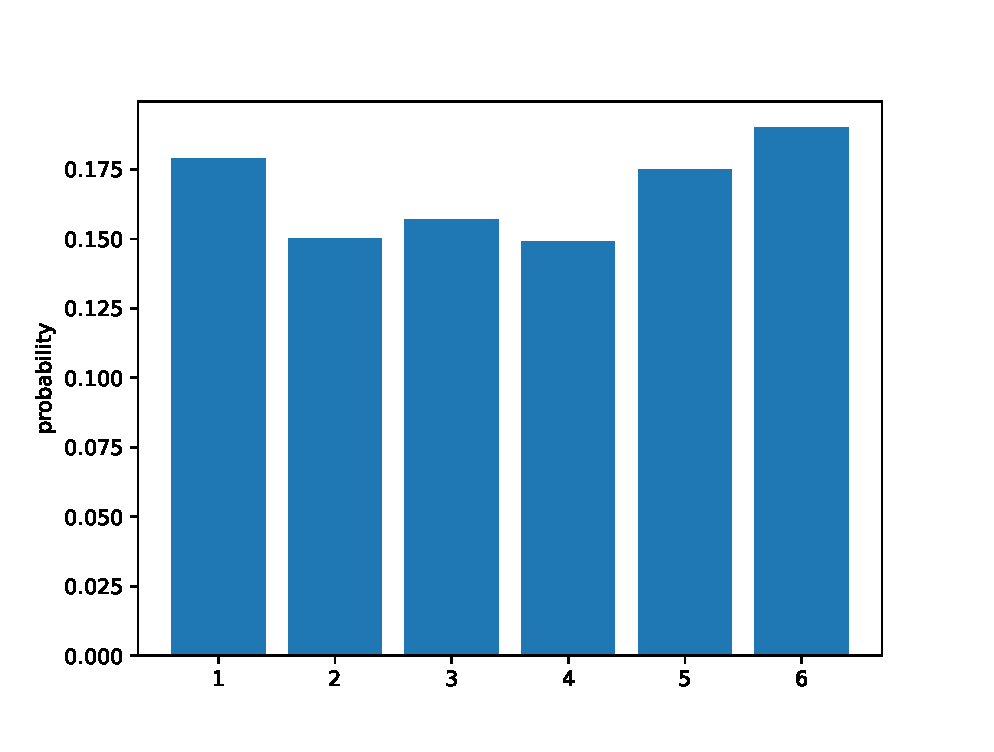
\includegraphics[width=\columnwidth]{./figures/probexm/probexm3.eps}
%	\caption{probability of outcome of biased dice }
%	\label{fig:bts3}
%	\begin{lstlisting}
%	figs/probexm/probexm3.eps
%	\end{lstlisting}
%\end{figure}


   \item The record of a weather station shows that out of the past 250 consecutive days, its weather forecasts were correct 175 times.\\
   (i) What is the probability that on a given day it was correct?\\
(ii) What is the probability that it was not correct on a given day?\\
\solution
Let $X \in \cbrak{0,1}$ be the random variable with 1 denoting correct forecast.
From the given information,
\begin{align}
\pr{X=1} & = \frac{175}{250}
\\
&= 0.7
\\
\pr{X=0} & = 1 - \pr{X=1}
\\
&= 0.3
\end{align}



\item {\em: Random Process}A and B throw a die alternatively till one of them gets a '6' and wins the game. Find their respective probabilities of winning, if A starts first.
\\
\solution
Let X be the random variable representing the number of defective eggs from the ten eggs picked. X follows a  binomial distribution.  Since the probability of an egg being defective is 10\%, substituting n=10, p= 0.1 and k=0 in equation \eqref{eq:exam41_1}, 
probability that there is atleast one defective egg is 
\begin{align}
\pr{X \geq 1}&= 1 - \pr{X=0}  = 1-\brak{0.9}^{10}
\\
&=0.6513215599
\end{align}
The python code for the above problem is,
\begin{lstlisting}
.solutions/20-10/prob/codes/exam42.py
\end{lstlisting}

%
\item To know the opinion of the students about the subject statistics, a survey of 200 students was conducted. The data is recorded in Table \ref{table:1.2.6}
Find the probability that a student chosen at random
\begin{enumerate}
\item likes statistics,
\item  does not like it.
\end{enumerate}
\begin{table}[!ht]
\centering
\begin{tabular}{ |c|c| } 
 \hline
 \textbf{Opinion} &\textbf{Number of students}\\
 \hline
 like  &135\\ 
 \hline
 dislike  &65\\ 
 \hline
\end{tabular}
\caption{}
\label{table:1.2.6}
\end{table}
\solution
Let X be the random variable representing the number of defective eggs from the ten eggs picked. X follows a  binomial distribution.  Since the probability of an egg being defective is 10\%, substituting n=10, p= 0.1 and k=0 in equation \eqref{eq:exam41_1}, 
probability that there is atleast one defective egg is 
\begin{align}
\pr{X \geq 1}&= 1 - \pr{X=0}  = 1-\brak{0.9}^{10}
\\
&=0.6513215599
\end{align}
The python code for the above problem is,
\begin{lstlisting}
.solutions/20-10/prob/codes/exam42.py
\end{lstlisting}

\item  Assume that each born child is equally likely to be a boy or a girl. If a family has two children, what is the conditional probability that both are girls given that\\
(i) the youngest is a girl,\\ 
(ii) at least one is a girl?\\
\solution

	\begin{table}[ht]
    \begin{center}
    	%%%%%%%%%%%%%%%%%%%%%%%%%%%%%%%%%%%%%%%%%%%%%%%%%%%%%%%%%%%%%%%%%%%%%%
%%                                                                  %%
%%  This is the header of a LaTeX2e file exported from Gnumeric.    %%
%%                                                                  %%
%%  This file can be compiled as it stands or included in another   %%
%%  LaTeX document. The table is based on the longtable package so  %%
%%  the longtable options (headers, footers...) can be set in the   %%
%%  preamble section below (see PRAMBLE).                           %%
%%                                                                  %%
%%  To include the file in another, the following two lines must be %%
%%  in the including file:                                          %%
%%        \def\inputGnumericTable{}                                 %%
%%  at the beginning of the file and:                               %%
%%        \input{name-of-this-file.tex}                             %%
%%  where the table is to be placed. Note also that the including   %%
%%  file must use the following packages for the table to be        %%
%%  rendered correctly:                                             %%
%%    \usepackage[latin1]{inputenc}                                 %%
%%    \usepackage{color}                                            %%
%%    \usepackage{array}                                            %%
%%    \usepackage{longtable}                                        %%
%%    \usepackage{calc}                                             %%
%%    \usepackage{multirow}                                         %%
%%    \usepackage{hhline}                                           %%
%%    \usepackage{ifthen}                                           %%
%%  optionally (for landscape tables embedded in another document): %%
%%    \usepackage{lscape}                                           %%
%%                                                                  %%
%%%%%%%%%%%%%%%%%%%%%%%%%%%%%%%%%%%%%%%%%%%%%%%%%%%%%%%%%%%%%%%%%%%%%%



%%  This section checks if we are begin input into another file or  %%
%%  the file will be compiled alone. First use a macro taken from   %%
%%  the TeXbook ex 7.7 (suggestion of Han-Wen Nienhuys).            %%
\def\ifundefined#1{\expandafter\ifx\csname#1\endcsname\relax}


%%  Check for the \def token for inputed files. If it is not        %%
%%  defined, the file will be processed as a standalone and the     %%
%%  preamble will be used.                                          %%
\ifundefined{inputGnumericTable}

%%  We must be able to close or not the document at the end.        %%
	\def\gnumericTableEnd{\end{document}}


%%%%%%%%%%%%%%%%%%%%%%%%%%%%%%%%%%%%%%%%%%%%%%%%%%%%%%%%%%%%%%%%%%%%%%
%%                                                                  %%
%%  This is the PREAMBLE. Change these values to get the right      %%
%%  paper size and other niceties.                                  %%
%%                                                                  %%
%%%%%%%%%%%%%%%%%%%%%%%%%%%%%%%%%%%%%%%%%%%%%%%%%%%%%%%%%%%%%%%%%%%%%%

	\documentclass[12pt%
			  %,landscape%
                    ]{report}
       \usepackage[latin1]{inputenc}
       \usepackage{fullpage}
       \usepackage{color}
       \usepackage{array}
       \usepackage{longtable}
       \usepackage{calc}
       \usepackage{multirow}
       \usepackage{hhline}
       \usepackage{ifthen}

	\begin{document}


%%  End of the preamble for the standalone. The next section is for %%
%%  documents which are included into other LaTeX2e files.          %%
\else

%%  We are not a stand alone document. For a regular table, we will %%
%%  have no preamble and only define the closing to mean nothing.   %%
    \def\gnumericTableEnd{}

%%  If we want landscape mode in an embedded document, comment out  %%
%%  the line above and uncomment the two below. The table will      %%
%%  begin on a new page and run in landscape mode.                  %%
%       \def\gnumericTableEnd{\end{landscape}}
%       \begin{landscape}


%%  End of the else clause for this file being \input.              %%
\fi

%%%%%%%%%%%%%%%%%%%%%%%%%%%%%%%%%%%%%%%%%%%%%%%%%%%%%%%%%%%%%%%%%%%%%%
%%                                                                  %%
%%  The rest is the gnumeric table, except for the closing          %%
%%  statement. Changes below will alter the table's appearance.     %%
%%                                                                  %%
%%%%%%%%%%%%%%%%%%%%%%%%%%%%%%%%%%%%%%%%%%%%%%%%%%%%%%%%%%%%%%%%%%%%%%

\providecommand{\gnumericmathit}[1]{#1} 
%%  Uncomment the next line if you would like your numbers to be in %%
%%  italics if they are italizised in the gnumeric table.           %%
%\renewcommand{\gnumericmathit}[1]{\mathit{#1}}
\providecommand{\gnumericPB}[1]%
{\let\gnumericTemp=\\#1\let\\=\gnumericTemp\hspace{0pt}}
 \ifundefined{gnumericTableWidthDefined}
        \newlength{\gnumericTableWidth}
        \newlength{\gnumericTableWidthComplete}
        \newlength{\gnumericMultiRowLength}
        \global\def\gnumericTableWidthDefined{}
 \fi
%% The following setting protects this code from babel shorthands.  %%
 \ifthenelse{\isundefined{\languageshorthands}}{}{\languageshorthands{english}}
%%  The default table format retains the relative column widths of  %%
%%  gnumeric. They can easily be changed to c, r or l. In that case %%
%%  you may want to comment out the next line and uncomment the one %%
%%  thereafter                                                      %%
\providecommand\gnumbox{\makebox[0pt]}
%%\providecommand\gnumbox[1][]{\makebox}

%% to adjust positions in multirow situations                       %%
\setlength{\bigstrutjot}{\jot}
\setlength{\extrarowheight}{\doublerulesep}

%%  The \setlongtables command keeps column widths the same across  %%
%%  pages. Simply comment out next line for varying column widths.  %%
\setlongtables

\setlength\gnumericTableWidth{%
	53pt+%
	53pt+%
	53pt+%
0pt}
\def\gumericNumCols{3}
\setlength\gnumericTableWidthComplete{\gnumericTableWidth+%
         \tabcolsep*\gumericNumCols*2+\arrayrulewidth*\gumericNumCols}
\ifthenelse{\lengthtest{\gnumericTableWidthComplete > \linewidth}}%
         {\def\gnumericScale{\ratio{\linewidth-%
                        \tabcolsep*\gumericNumCols*2-%
                        \arrayrulewidth*\gumericNumCols}%
{\gnumericTableWidth}}}%
{\def\gnumericScale{1}}

%%%%%%%%%%%%%%%%%%%%%%%%%%%%%%%%%%%%%%%%%%%%%%%%%%%%%%%%%%%%%%%%%%%%%%
%%                                                                  %%
%% The following are the widths of the various columns. We are      %%
%% defining them here because then they are easier to change.       %%
%% Depending on the cell formats we may use them more than once.    %%
%%                                                                  %%
%%%%%%%%%%%%%%%%%%%%%%%%%%%%%%%%%%%%%%%%%%%%%%%%%%%%%%%%%%%%%%%%%%%%%%

\ifthenelse{\isundefined{\gnumericColA}}{\newlength{\gnumericColA}}{}\settowidth{\gnumericColA}{\begin{tabular}{@{}p{53pt*\gnumericScale}@{}}x\end{tabular}}
\ifthenelse{\isundefined{\gnumericColB}}{\newlength{\gnumericColB}}{}\settowidth{\gnumericColB}{\begin{tabular}{@{}p{53pt*\gnumericScale}@{}}x\end{tabular}}
\ifthenelse{\isundefined{\gnumericColC}}{\newlength{\gnumericColC}}{}\settowidth{\gnumericColC}{\begin{tabular}{@{}p{53pt*\gnumericScale}@{}}x\end{tabular}}

\begin{tabular}[c]{%
	b{\gnumericColA}%
	b{\gnumericColB}%
	b{\gnumericColC}%
	}

%%%%%%%%%%%%%%%%%%%%%%%%%%%%%%%%%%%%%%%%%%%%%%%%%%%%%%%%%%%%%%%%%%%%%%
%%  The longtable options. (Caption, headers... see Goosens, p.124) %%
%	\caption{The Table Caption.}             \\	%
% \hline	% Across the top of the table.
%%  The rest of these options are table rows which are placed on    %%
%%  the first, last or every page. Use \multicolumn if you want.    %%

%%  Header for the first page.                                      %%
%	\multicolumn{3}{c}{The First Header} \\ \hline 
%	\multicolumn{1}{c}{colTag}	%Column 1
%	&\multicolumn{1}{c}{colTag}	%Column 2
%	&\multicolumn{1}{c}{colTag}	\\ \hline %Last column
%	\endfirsthead

%%  The running header definition.                                  %%
%	\hline
%	\multicolumn{3}{l}{\ldots\small\slshape continued} \\ \hline
%	\multicolumn{1}{c}{colTag}	%Column 1
%	&\multicolumn{1}{c}{colTag}	%Column 2
%	&\multicolumn{1}{c}{colTag}	\\ \hline %Last column
%	\endhead

%%  The running footer definition.                                  %%
%	\hline
%	\multicolumn{3}{r}{\small\slshape continued\ldots} \\
%	\endfoot

%%  The ending footer definition.                                   %%
%	\multicolumn{3}{c}{That's all folks} \\ \hline 
%	\endlastfoot
%%%%%%%%%%%%%%%%%%%%%%%%%%%%%%%%%%%%%%%%%%%%%%%%%%%%%%%%%%%%%%%%%%%%%%

\hhline{|-|-~}
	 \multicolumn{1}{|p{\gnumericColA}|}%
	{\gnumericPB{\centering}\gnumbox{Mark}}
	&\multicolumn{1}{p{\gnumericColB}|}%
	{\gnumericPB{\centering}\gnumbox{Frequency}}
	&
\\
\hhline{|--|~}
	 \multicolumn{1}{|p{\gnumericColA}|}%
	{\gnumericPB{\centering}\gnumbox{2}}
	&\multicolumn{1}{p{\gnumericColB}|}%
	{\gnumericPB{\centering}\gnumbox{1}}
	&
\\
\hhline{|--|~}
	 \multicolumn{1}{|p{\gnumericColA}|}%
	{\gnumericPB{\centering}\gnumbox{3}}
	&\multicolumn{1}{p{\gnumericColB}|}%
	{\gnumericPB{\centering}\gnumbox{2}}
	&
\\
\hhline{|--|~}
	 \multicolumn{1}{|p{\gnumericColA}|}%
	{\gnumericPB{\centering}\gnumbox{4}}
	&\multicolumn{1}{p{\gnumericColB}|}%
	{\gnumericPB{\centering}\gnumbox{3}}
	&
\\
\hhline{|--|~}
	 \multicolumn{1}{|p{\gnumericColA}|}%
	{\gnumericPB{\centering}\gnumbox{5}}
	&\multicolumn{1}{p{\gnumericColB}|}%
	{\gnumericPB{\centering}\gnumbox{2}}
	&
\\
\hhline{|--|~}
	 \multicolumn{1}{|p{\gnumericColA}|}%
	{\gnumericPB{\centering}\gnumbox{6}}
	&\multicolumn{1}{p{\gnumericColB}|}%
	{\gnumericPB{\centering}\gnumbox{3}}
	&
\\
\hhline{|--|~}
	 \multicolumn{1}{|p{\gnumericColA}|}%
	{\gnumericPB{\centering}\gnumbox{7}}
	&\multicolumn{1}{p{\gnumericColB}|}%
	{\gnumericPB{\centering}\gnumbox{3}}
	&
\\
\hhline{|--|~}
	 \multicolumn{1}{|p{\gnumericColA}|}%
	{\gnumericPB{\centering}\gnumbox{9}}
	&\multicolumn{1}{p{\gnumericColB}|}%
	{\gnumericPB{\centering}\gnumbox{4}}
	&
\\
\hhline{|--|~}
	 \multicolumn{1}{|p{\gnumericColA}|}%
	{\gnumericPB{\centering}\gnumbox{10}}
	&\multicolumn{1}{p{\gnumericColB}|}%
	{\gnumericPB{\centering}\gnumbox{2}}
	&
\\
\hhline{|-|-|~}
\end{tabular}

\ifthenelse{\isundefined{\languageshorthands}}{}{\languageshorthands{\languagename}}
\gnumericTableEnd

  \caption{Marks obtained by students}
   \label{table:statsex_23table1}
   \end{center}	
\end{table}

As we can see from table \ref{table:statsex_23table1}, 9 occurs the maximum number of times.\\
Thus Mode = 9.




\item  An instructor has a question bank consisting of 300 easy True / False questions,
200 difficult True / False questions, 500 easy multiple choice questions and 400 difficult multiple choice questions. If a question is selected at random from the question bank, what is the probability that it will be an easy question given that it is a multiple choice question?\\
\solution
From the given information, using the fact that $A,B$ are independent,
\begin{align}
\pr{A+B} &= \pr{A}+\pr{B}-\pr{AB}
\\
&= \pr{A} + \pr{B-AB} 
\\
&= \pr{A} + \pr{A'B}
\\
&= \pr{A} + \pr{A'}\pr{B}
\\
&= \pr{A} + \pr{A'}\brak{1-\pr{B'}}
\\
&= \pr{A} + \pr{A'}-\pr{A'}\pr{B'}
\\
&=1 - \pr{A'}\pr{B'}
\end{align}


\item Two cards are drawn at random and without replacement from a pack of 52 playing cards. Find the probability that both the cards are black.\\
\solution
Let $X_1,X_2 \in \cbrak{0,1}$ represent the colour, where 0 denotes black and 1 denotes red.  From the given information,
\begin{align}
\pr{X_1 = 0} &= \frac{26}{52}= \frac{1}{2}
\\
\pr{X_2 = 0|X_1 = 0} &= \frac{25}{51}
\end{align}
Then,
\begin{multline}
\pr{X_1=0,X_2=0} 
\\
= \pr{X_2 = 0|X_1 = 0}\pr{X_1 = 0}
 = \frac{25}{102}
\end{multline}

\item Two balls are drawn at random with replacement from a box containing 10 black and 8 red balls. Find the probability that\\
(i) both balls are red.\\
(ii) first ball is black and second is red.\\
(iii) one of them is black and other is red.\\
\solution
Let X be the random variable representing the number of defective eggs from the ten eggs picked. X follows a  binomial distribution.  Since the probability of an egg being defective is 10\%, substituting n=10, p= 0.1 and k=0 in equation \eqref{eq:exam41_1}, 
probability that there is atleast one defective egg is 
\begin{align}
\pr{X \geq 1}&= 1 - \pr{X=0}  = 1-\brak{0.9}^{10}
\\
&=0.6513215599
\end{align}
The python code for the above problem is,
\begin{lstlisting}
.solutions/20-10/prob/codes/exam42.py
\end{lstlisting}


\item Probability of solving specific problem independently by A and B are $\frac{1}{2}$
and $\frac{1}{3}$ respectively. If both try to solve the problem independently, find the probability that\\
(i) the problem is solved \\
(ii) exactly one of them solves the problem.\\
\solution
Let X be the random variable representing the number of defective eggs from the ten eggs picked. X follows a  binomial distribution.  Since the probability of an egg being defective is 10\%, substituting n=10, p= 0.1 and k=0 in equation \eqref{eq:exam41_1}, 
probability that there is atleast one defective egg is 
\begin{align}
\pr{X \geq 1}&= 1 - \pr{X=0}  = 1-\brak{0.9}^{10}
\\
&=0.6513215599
\end{align}
The python code for the above problem is,
\begin{lstlisting}
.solutions/20-10/prob/codes/exam42.py
\end{lstlisting}

\item (i) A lot of 20 bulbs contain 4 defective ones. One bulb is drawn at random from the lot.
What is the probability that this bulb is defective?\\
(ii) Suppose the bulb drawn in (i) is not defective and is not replaced. Now one bulb
is drawn at random from the rest. What is the probability that this bulb is not
defective ?
\\
\solution
Let X be the random variable representing the number of defective eggs from the ten eggs picked. X follows a  binomial distribution.  Since the probability of an egg being defective is 10\%, substituting n=10, p= 0.1 and k=0 in equation \eqref{eq:exam41_1}, 
probability that there is atleast one defective egg is 
\begin{align}
\pr{X \geq 1}&= 1 - \pr{X=0}  = 1-\brak{0.9}^{10}
\\
&=0.6513215599
\end{align}
The python code for the above problem is,
\begin{lstlisting}
.solutions/20-10/prob/codes/exam42.py
\end{lstlisting}

\item 12 defective pens are accidentally mixed with 132 good ones. It is not possible to just
look at a pen and tell whether or not it is defective. One pen is taken out at random from
this lot. Determine the probability that the pen taken out is a good one.
\\
\solution
Let X be the random variable representing the number of defective eggs from the ten eggs picked. X follows a  binomial distribution.  Since the probability of an egg being defective is 10\%, substituting n=10, p= 0.1 and k=0 in equation \eqref{eq:exam41_1}, 
probability that there is atleast one defective egg is 
\begin{align}
\pr{X \geq 1}&= 1 - \pr{X=0}  = 1-\brak{0.9}^{10}
\\
&=0.6513215599
\end{align}
The python code for the above problem is,
\begin{lstlisting}
.solutions/20-10/prob/codes/exam42.py
\end{lstlisting}

\item Gopi buys a fish from a shop for his aquarium. The
shopkeeper takes out one fish at random from a
tank containing 5 male fish and 8 female fish (see
Fig. \ref{fig:prob_121}). What is the probability that the fish taken
out is a male fish?
\begin{figure}[!ht]
\centering
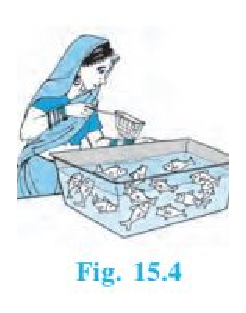
\includegraphics[width=\columnwidth]{./prob/figs/woman.eps}
\caption{}
\label{fig:prob_121}
\end{figure}
\\
\solution
Let X be the random variable representing the number of defective eggs from the ten eggs picked. X follows a  binomial distribution.  Since the probability of an egg being defective is 10\%, substituting n=10, p= 0.1 and k=0 in equation \eqref{eq:exam41_1}, 
probability that there is atleast one defective egg is 
\begin{align}
\pr{X \geq 1}&= 1 - \pr{X=0}  = 1-\brak{0.9}^{10}
\\
&=0.6513215599
\end{align}
The python code for the above problem is,
\begin{lstlisting}
.solutions/20-10/prob/codes/exam42.py
\end{lstlisting}
    
\item A lot consists of 144 ball pens of which 20 are defective and the others are good. Nuri will buy a pen if it is good, but will not buy if it is defective. The shopkeeper draws one pen at random and gives it to her. What is the probability that\\
(i) She will buy it ?\\
(ii) She will not buy it ?
\\
\solution
Let X be the random variable representing the number of defective eggs from the ten eggs picked. X follows a  binomial distribution.  Since the probability of an egg being defective is 10\%, substituting n=10, p= 0.1 and k=0 in equation \eqref{eq:exam41_1}, 
probability that there is atleast one defective egg is 
\begin{align}
\pr{X \geq 1}&= 1 - \pr{X=0}  = 1-\brak{0.9}^{10}
\\
&=0.6513215599
\end{align}
The python code for the above problem is,
\begin{lstlisting}
.solutions/20-10/prob/codes/exam42.py
\end{lstlisting}


\item A bag contains 5 red balls and some blue balls. If the probability of drawing a blue ball is double that of a red ball, determine the number of blue balls in the bag.
\\
\solution
Let X be the random variable representing the number of defective eggs from the ten eggs picked. X follows a  binomial distribution.  Since the probability of an egg being defective is 10\%, substituting n=10, p= 0.1 and k=0 in equation \eqref{eq:exam41_1}, 
probability that there is atleast one defective egg is 
\begin{align}
\pr{X \geq 1}&= 1 - \pr{X=0}  = 1-\brak{0.9}^{10}
\\
&=0.6513215599
\end{align}
The python code for the above problem is,
\begin{lstlisting}
.solutions/20-10/prob/codes/exam42.py
\end{lstlisting}

\item A box contains 12 balls out of which x are black. If one ball is drawn at random from the box,what is the probability that it will be a black ball?\\
If 6 more black balls are put in the box, the probability of drawing a black ball is now double of what it was before. Find x.
\\
\solution
Let X be the random variable representing the number of defective eggs from the ten eggs picked. X follows a  binomial distribution.  Since the probability of an egg being defective is 10\%, substituting n=10, p= 0.1 and k=0 in equation \eqref{eq:exam41_1}, 
probability that there is atleast one defective egg is 
\begin{align}
\pr{X \geq 1}&= 1 - \pr{X=0}  = 1-\brak{0.9}^{10}
\\
&=0.6513215599
\end{align}
The python code for the above problem is,
\begin{lstlisting}
.solutions/20-10/prob/codes/exam42.py
\end{lstlisting}

\end{enumerate}
%\end{document}
    
 
\section{Bayes Rule}
\renewcommand{\theequation}{\theenumi}
\begin{enumerate}[label=\thesection.\arabic*.,ref=\thesection.\theenumi]
\numberwithin{equation}{enumi}


\item Bag I contains 3 red and 4 black balls and Bag II contains 4 red and 5 black balls. One ball is transferred from Bag I to Bag II and then a ball is drawn from Bag II. The ball so drawn is found to be red in colour. Find the probability that the transferred ball is black.\\
\item Suppose we have four boxes A,B,C and D containing coloured marbles as given below:\\
\\$\begin{tabular}{||c c c c||} 
 \hline
 Box & Red & White & Black \\
 \hline
 A & 1 & 6 & 3 \\
 \hline
 B & 6 & 2 & 2 \\
 \hline
 C & 8 & 1 & 1 \\
 \hline
 D & 0 & 6 & 4 \\
 \hline
\end{tabular}$\\
\\One of the boxes has been selected at random and a single marble is drawn from
it. If the marble is red, what is the probability that it was drawn from box A?, box B?,
box C?\\
\solution 
The description of the random variables is available in Table \ref{table:2.2}.
\begin{table}[!ht]
\centering
\begin{tabular}{|c|c|c|c|c|}
\hline
     &A&B&C&D  \\
     \hline
     X&0&1&2&3\\
     \hline
\end{tabular}\\[5pt]
\begin{tabular}{|c|c|c|c|}
\hline
     &Red&White&Black  \\
     \hline
     Y&0&1&2\\
     \hline
\end{tabular}\\[5pt]
\caption{}
\label{table:2.2}
\end{table}
From the given information,
\begin{align}
\pr{X\!=\!0} = \pr{X\!=\!1} &= \pr{X\!=\!2} 
\\
= \pr{X\!=\!3} &= \frac{1}{4}
\\
\pr{Y\!=\!0|X\!=\!0}&=\frac{1}{10}\\
\\\pr{Y\!=\!0|X\!=\!1}&=\frac{6}{10}\\
\\\pr{Y\!=\!0|X\!=\!2}&=\frac{8}{10}\\
\pr{Y\!=\!0|X\!=\!3} &=0
\end{align}
Thus,
\begin{align}
\pr{Y=0}&= \sum_{i=0}^{3}\pr{Y=0|X=i}\pr{X=i}
\\
&=\frac{3}{8}
\end{align}
\begin{enumerate}
\item  
\begin{multline}
Pr(X=0|Y=0)
\\
=\frac{{Pr(Y=0|X=0)}{Pr(X=0)}}{{Pr(Y=0)}}
\\
=\frac{1}{15}
\end{multline}
\item 
\begin{multline}
Pr(X=1|Y=0)
\\
=\frac{{Pr(Y=0|X=1)}{Pr(X=1)}}{{Pr(Y=0)}}
\\
=\frac{2}{5}
\end{multline}
\item 
\begin{multline}
Pr(X=2|Y=0)
\\=\frac{{Pr(Y=0|X=2)}{Pr(X=2)}}{{Pr(Y=0)}}
\\
=\frac{8}{15}
\end{multline}
\end{enumerate}

\item Assume that the chances of a patient having a heart attack is 40$\%$. It is also
assumed that a meditation and yoga course reduce the risk of heart attack by 30$\%$ and prescription of certain drug reduces its chances by 25$\%$. At a time a patient can choose any one of the two options with equal probabilities. It is given that after going through one of the two options the patient selected at random suffers a heart attack. Find the probability that the patient followed a course of meditation and yoga?\\
\solution
Let $H \in \{ 0, 1\}$ denote the random variable of the patient having a heart attack, $A \in \{ 0, 1\} $ denote the random variable of the patient taking a meditation and yoga course, or the patient taking the drug. ($A=0$ if the patient took a meditation and yoga course, and $A=1$ if the patient took the prescription of the drug.)\\
Given that,
\begin{align}
\text{Pr}(H=1) &= 0.4 \\
\text{Pr}(A=0) &= \text{Pr}(A=1)\\
\text{Pr}(H=1|A=0) &= \text{Pr}(H=1)\,(1-0.30)\\
&= 0.28 \\
\text{Pr}(H=1|A=1) &= \text{Pr}(H=1)\,(1-0.25)\\
&= 0.3\\
\end{align}
Therefore, by Bayes' Theorem
\begin{align}
\text{Pr}(A=0|H=1) = \dfrac{\text{Pr}(H=1|A=0)\,\text{Pr}(A=0)}{\sum_{i=0} ^ 1 \text{Pr}(H=1|A=i)\,\text{Pr}(A=i)} \\
\end{align}
We can cancel $\text{Pr}(A=1)$ and $\text{Pr}(A=0)$ from the numerator and denominator as they are given to be equal.\\
\begin{align}
\therefore \text{Pr}(A=0|H=1) &= \dfrac{\text{Pr}(H=1|A=0)}{\text{Pr}(H=1|A=0) + \text{Pr}(H=1|A=1)} \\
&= \dfrac{0.28}{0.28 + 0.3} \\ ~\\[-1em]
&= \dfrac{0.28}{0.58} \\ ~\\[-1em]
&= \dfrac{14}{29} \\ ~\\[-1em]
&\approx 0.48275862069
\end{align}
\item Suppose that 5$\%$ of men and 0.25$\%$ of women have grey hair. A grey haired person is selected at random. What is the probability of this person being male? Assume that there are equal number of males and females.\\
\solution
Say there are 100 people. Half of them men and half of them women. 5\% of men have grey hair(2.5 men) and 0.25\% of women have grey hair(0.125 women)


\begin{center}
\begin{tabular}{ |c|c|c|c| } 
\hline
 & \textbf{Men} & \textbf{Women} & \textbf{Total} \\
\hline
 & 50 & 50 & 100 \\ 
\hline
\textbf{Greyhair} & 2.5 & 0.125 & \\ 
 \hline
\end{tabular}
\end{center}


 Required probability = how many of men have grey hair = $\frac{\textbf{Men with grey hair}}{\textbf{total grey haired persons}} \\ = \frac{2.5}{2.5+0.125} \\ = \frac{2.5}{2.625} \\ = \textbf{0.95238} $ 
 
\textbf{ Another way using Bayes theorem}:

M - No of men, W = No of women , G = No of grey persons
$P(M) = 0.5 = P(W) \\ P(G|M) =0.05 \\ P(G|W) = 0.0025 \\ P(M|G) \textbf{ is what we need to find } $

\textbf{By bayes theorem}, 
\begin{multline*}
%\begin{equation} 
\begin{split}
P(M|G) & = \frac{P(M,G)}{P(G)} \\
 & = \frac{P(G|M)P(M)}{P(G)} \\
 & = \frac{P(G|M)P(M)}{P(G|M)P(M)+P(G|W)P(W)} \\
 & = \frac{0.05*0.5}{0.05*0.5+0.0025*0.5} \\
 & = \frac{0.025}{0.02625} \\
 & = \textbf{0.95238}
\end{split}
%\end{equation}
\end{multline*}
        

%Say there are 100 people. Half of them men and half of them women. 5\% of men have grey hair(2.5 men) and 0.25\% of women have grey hair(0.125 women)


\begin{center}
\begin{tabular}{ |c|c|c|c| } 
\hline
 & \textbf{Men} & \textbf{Women} & \textbf{Total} \\
\hline
 & 50 & 50 & 100 \\ 
\hline
\textbf{Greyhair} & 2.5 & 0.125 & \\ 
 \hline
\end{tabular}
\end{center}


 Required probability = how many of men have grey hair = $\frac{\textbf{Men with grey hair}}{\textbf{total grey haired persons}} \\ = \frac{2.5}{2.5+0.125} \\ = \frac{2.5}{2.625} \\ = \textbf{0.95238} $ 
 
\textbf{ Another way using Bayes theorem}:

M - No of men, W = No of women , G = No of grey persons
$P(M) = 0.5 = P(W) \\ P(G|M) =0.05 \\ P(G|W) = 0.0025 \\ P(M|G) \textbf{ is what we need to find } $

\textbf{By bayes theorem}, 
\begin{multline*}
%\begin{equation} 
\begin{split}
P(M|G) & = \frac{P(M,G)}{P(G)} \\
 & = \frac{P(G|M)P(M)}{P(G)} \\
 & = \frac{P(G|M)P(M)}{P(G|M)P(M)+P(G|W)P(W)} \\
 & = \frac{0.05*0.5}{0.05*0.5+0.0025*0.5} \\
 & = \frac{0.025}{0.02625} \\
 & = \textbf{0.95238}
\end{split}
%\end{equation}
\end{multline*}
        


\item A couple has two children,\\
(i) Find the probability that both children are males, if it is known that at least one of the children is male.\\
(ii) Find the probability that both children are females, if it is known that the elder child is a female.\\
\item A manufacturer has three machine operators A, B and C. The first operator A
produces 1$\%$ defective items, where as the other two operators B and C produce 5$\%$ and 7$\%$ defective items respectively. A is on the job for 50$\%$ of the time, B is on the job for 30$\%$ of the time and C is on the job for 20$\%$ of the time. A defective item is produced, what is the probability that it was produced by A?\\
\solution
Let X $\in\{0,1,2\}$ be the random variable denoting that item was produced by operator A when X$=$0, X$=$1 denoting that item was produced by operator B ,X$=$2 denoting that item was produced by operator C, and random variable Y $\in\{0,1\}$ be the random variable deoting that item produced was  defective when Y$=$1.
\begin{align}
	\pr{X=0} &= 0.5 \\ 
    \pr{X=1} &= 0.3 \\ 
    \pr{X=2} &= 0.2 \\ 
	\pr{Y=1/X=0} &= 0.01\\
	\pr{Y=1/X=1} &= 0.05\\ 
	\pr{Y=1/X=2} &= 0.07
	\end{align}
	%
	From conditional probability we say that \\
	\begin{align*}
	\pr{X=0/Y=1} &= \frac{\pr{Y=1/X=0}\pr{X=0}}{\sum_{i=0}^{i=2}\pr{Y=1/X=i}\pr{X=i}}\\
	&=\frac{5}{34}
	\end{align*}


\item A factory has two machines A and B. Past record shows that machine A produced 60$\%$ of the items of output and machine B produced 40$\%$ of the items. Further, 2$\%$ of the items produced by machine A and 1$\%$ produced by machine B were defective. All the items are put into one stockpile and then one item is chosen at random from this and is found to be defective. What is the probability that it was produced by machine B?\\
%
\solution
Let $A \in \cbrak{0,1}$ denote the random variables of an item produced and $D \cbrak{0,1}$ denote it being defective
%
From the given information,
\begin{align}
P(A=0) = 60 {\%} = 0.6\\
P(A=1) = 40 {\%} =0.4
\end{align}
\begin{align}
    P(D=1|A=0) = P(1|0) = 2 {\%} =0.02
   \\P(D=1|A=1) = P(1|1) =  1 {\%} =0.01
\end{align}
By Baye's rule,
\begin{multline}
    P(A=1|D=1) 
    \\
    = \frac{P(1)\times P(1|1)}{P(1)\times P(1|1) + P(0)\times P(1|0)}
    \\P(A=1|D=1) = \frac{0.4\times 0.01}{0.4\times 0.01 + 0.6\times 0.02}
    \\P(A=1|D=1) = 0.25
\end{multline}
The probability that the defective item selected at random is produced by machine B is 25{\%}
\item Two groups are competing for the position on the Board of directors of a corporation. The probabilities that the first and the second groups will win are 0.6 and 0.4 respectively. Further, if the first group wins, the probability of introducing a new product is 0.7 and the corresponding probability is 0.3 if the second group wins. Find the probability that the new product introduced was by the second group.\\
%
\solution
let $M \in \{0,1\}$ be a random variable such that $M=0$ represents product is not introduced by winning group and $M=1$ represents product is introduced by the winning group.let $H \in \{0,1\}$ be another random variable such that $H=0$ represents that group A wins,$H=1$ represents that group B wins.
\begin{table}[h]
\centering 
\caption{}
\begin{tabular}{|c|c|}
\hline
variable & description \\
\hline
$M = 0$  &not introduced by winning group \\
\hline
$M = 1$  &introduced by winning group \\
\hline
$H = 0$  & group A wins \\
\hline
$H = 1$  & group B wins \\
\hline
\end{tabular}
\label{bayes/2/8/table:}
\end{table}
\begin{table}[h]
\centering 
\caption{}
\begin{tabular}{|c|c|c|}
\hline
           & $H = 0$  & $H = 1$\\
\hline
$M = 0$  & o.18  & 0.28 \\
\hline
$M = 1$  & 0.42    &  0.12 \\
\hline
\end{tabular}
\label{bayes/2/8/table:}
\end{table}
we know that Bayes theorem:
\begin{align}
P(A|B)=\frac{P(A\cap B)}{P(B)} ,ifP(B)\neq 0.
\end{align}
so required probability that new product was introduced by group B be P.
\begin{align}
 P=Pr(M=0|H=0)+Pr(M=1|H=1)\\
 =0.18+0.12 \\ 
 =0.30\\
\end{align}
hence the required probability that the product was introduced by the second group is 0.30

\item A laboratory blood test is 99$\%$ effective in detecting a certain disease when it is in fact, present. However, the test also yields a false positive result for 0.5$\%$ of the healthy person tested (i.e. if a healthy person is tested, then, with probability 0.005, the test will imply he has the disease). If 0.1 percent of the population actually has the disease, what is the probability that a person has the disease given that his test result is positive?\\
\item A family has two children. What is the probability that both the children are boys given that at least one of them is a boy?\\
%
\solution
X - Random variable for number of boys.
$$X = \{0, 1, 2\}$$
where $n = 2$ and $p = \frac{1}{2}$
\begin{table}[h]
    \centering
    \begin{tabular}{|c|c|}
         \hline
        \textbf{X = x}&\textbf{\pr{X = x}} \\
        \hline    
         {X = 0} & {${^2 C _0} \times {q^2}$}\\
         \hline
         {X = 1} & {${^2 C _1} \times {q} \times {p}$}\\
         \hline
         {X = 2} & {${^2 C _2} \times {p^2}$}\\
         \hline
    \end{tabular}
\end{table}
\\
To find $\pr{X = 2\, | \,X \geq 1}$.
\begin{align}
    \pr{X = 2\, | \,X \geq 1} &= \dfrac{\pr{X = 2}}{\pr{X\geq 1}}\\
    &= \dfrac{\frac{1}{4}}{\frac{3}{4}}\\
    &= \dfrac{1}{3}
\end{align}
\item Ten cards numbered 1 to 10 are placed in a box, mixed up thoroughly and then one card is drawn randomly. If it is known that the number on the drawn card is more than 3, what is the probability that it is an even number?\\
\solution
The set of sample space which contains cards numbered from 1 to 10 be 
\begin{align}
S \in \{1,2,3,4,5,6,7,8,9,10\}
\end{align}
Now probability of picking a random card from ten cards is be $Pr(x)$. Then,
\begin{align}
Pr(x\in S )=\frac{1}{10}
\end{align}
Let the Set of Even numbered cards be $E$ and Set of cards numbered greater than 3 is $A$.
and we know that the set of even numbers from 1 to 10 is \{2,4,6,8,10\} . Then,
\begin{align}
E \in \{2,4,6,8,10\}    
\end{align}
Now here, The Set of numbers greater than 3 
is \{4,5,6,7,8,9,10\}. Then,
\begin{align}
    A \in \{4,5,6,7,8,9,10\}
\end{align}
\begin{align}
    Pr(A)=\frac{No.\; of\; elements\; in\; (A).}{Number\; of\; cards.}
\end{align}
\begin{align}
\label{2.11:eq1}
    Pr(A)=\frac{7}{10}=0.7
\end{align}
Now, the favoured outcomes are set of $EA$ and 
Here the set $EA$ contains the cards which are even and numbered greater than 3.
\begin{align}
    Pr(EA)=\frac{No.\; of\; elements\; in\; E A.}{Number\; of\;cards.}
\end{align}
\begin{align}
   Now , Pr(EA) = Pr(4)+Pr(6)+Pr(8)+Pr(10)
\end{align}
\begin{align}
\label{2.11:eq2}
     Pr(EA) =\frac{4}{10}=0.4 
\end{align}
The probability that the card drawn is even number which is greater than 3 is
\begin{align}
    Pr(E|A)=\frac{Pr(EA)}{Pr(A)}
\end{align}
Now,using (\ref{2.11:eq1}) and (\ref{2.11:eq2}). 
\begin{align}
  (\because Pr(EA)=0.4\; and \; Pr(A)=0.7)  
\end{align}
\begin{align}
And, Pr(E|A)=\frac{Pr(EA)}{Pr(A)}
\end{align}
\begin{align}
=\frac{0.4}{0.7}
\end{align}
\begin{align}
\therefore Pr(E|A)=\frac{4}{7}    
\end{align}
\begin{align}
\therefore Pr(E|A)=0.5714285714285714    
\end{align}

\item In a school, there are 1000 students, out of which 430 are girls. It is known that out of 430,  10 percentage of the girls study in class XII. What is the probability that a student chosen randomly studies in Class XII given that the chosen student is a girl?\\
\solution
Total number of students : 1000 \\
Total number of girls : 430  \\
Total number of girls in Class XII : 10 \% of total girls 
\begin{align}
=\frac{10}{100}\times 430 =43
\end{align}
Let X $\in$ $\{0,1\}$ be the random variable such that 1 represents girl, 0 represents boy.
\begin{table}[ht]
\caption{Probability distribution for values of X}
\label{2.12:table:0}
\begin{center}
\begin{tabular}{|c|c|}
    \hline
    X & P(X) \\
    \hline
    1 & 430/1000\\
    \hline
    0 & 570/100\\
    \hline
    \end{tabular} 
\end{center}   
\end{table}

Let Y $\in$ $\{0,1\}$ be the random variable such that 1 represents chosen student is in Class XII, 0 represents chosen student is not in Class XII.

\begin{table}[ht]
\caption{Probability distribution for values of Y}
\label{2.12:table:1}
\begin{center}
    \begin{tabular}{|c|c|}
    \hline
    Y & P(Y)\\
    \hline
    1 & $\frac{1}{2}$ \\
    \hline
    0 & $\frac{1}{2}$\\
    \hline
    \end{tabular}
\end{center} 
\end{table}
We require P(Y=1 $\vert$ X=1) (using Baye's theorem)
\begin{align}
=\dfrac{P(X=1\vert Y=1)\cdot P(Y=1)}{\sum_{i=0}^{1} P(X=1\vert Y=i)\cdot P(Y=i)}
\end{align}
\begin{center} 
=$\frac{P(X=1 \vert Y=1)P\brak(Y=1)}{\splitfrac{P(X=1\vert Y=0)P(Y=0)}{+P(X=1\vert Y=1)P(Y=1)}}$
\end{center}
\begin{table}[ht]
\caption{Probability for different values of X,Y}
\label{2.12:table:2}
\begin{center}
    \begin{tabular}{|c|c|c|}
    \hline
    Probability & Chosen Student & Value\\
    \hline
    $P(X=1\vert Y=0)$ & girl not in Class XII & $\frac{387}{1000}$\\
    \hline
    $ P(X=1\vert Y=1)$ & girl in Class XII & $\frac{43}{1000}$ \\
    \hline
    \end{tabular}
\end{center}    
\end{table} 
\begin{align}
&=\left[\dfrac{\brak( \frac{43}{1000}\times \frac{1}{2})}{\brak( \frac{387}{1000})\times \frac{1}{2}) + \brak( \frac{43}{1000}\times \frac{1}{2})}\right]\\
&=\dfrac{1}{10}\\ 
&=0.1
\end{align}

\item A die is thrown three times. Events A and B are defined as below:\\
A : 4 on the third throw.\\
B : 6 on the first and 5 on the second throw.\\
Find the probability of A given that B has already occurred?\\
\solution
Let $X_i \in \{1,2,3,4,5,6\}$ where $i=1,2,3$
be the random variables representing the outcomes of throwing a die three times.\\
\begin{enumerate}
\item Probability of event A happening=Probability of $X_3=4$
\begin{align}
    \Pr{(A)}=\Pr{(X_3=4)}
\end{align}
Since all the outcomes are equally likely their probabilities are same \\
so
\begin{align}
    \Pr{(A)}=\Pr{(X_3=4)}=\frac{1}{6}
    \label{2.13:eq:0.0.2}
\end{align}
\item Probability of event B happening=Probability of $X_1=6,X_2=5$.\\
so
\begin{align}
    \Pr{(B)}=\Pr{(X_1=6,X_2=5)}
\end{align}
Random variable $X_1$ depends on first throw of die and random variable $X_2$ depends on second throw of die so $X_1$ and $X_2$ are independent.\\
so 
\begin{align}
\begin{split}
    \Pr{(X_1=6,X_2=5)} &=\Pr{(X_1=6)} \Pr{(X_2=5)}\\
   &=\frac{1}{6}\times \frac{1}{6}=\frac{1}{36}
   \end{split}
\end{align}
\begin{align}
    \Pr{(B)}=\Pr{(X_1=6,X_2=5)}=\frac{1}{36}
    \label{2.13:eq:0.0.5}
\end{align}
Also A,B are also independent events \\
therefore  from \eqref{2.13:eq:0.0.2} and \eqref{2.13:eq:0.0.5}
\begin{align}
    \Pr{(AB)} = \Pr{(A)} \Pr{(B)}
     =\frac{1}{6} \times \frac{1}{36}
    \end{align}
    \begin{align}
 \implies  \Pr{(AB)}=\frac{1}{216}\label{2.13:eq:0.0.7}
\end{align}
Since we have to find probability of A given that B has already happened.\\
so $\Pr{(A|B)}$\\
\item By formula of conditional probability
\begin{align}
    \Pr{(A|B)}=\frac{\Pr{(AB)}}{\Pr{(B)}}
    \end{align}
    From \eqref{2.13:eq:0.0.5} and \eqref{2.13:eq:0.0.7} 
    \begin{align}  
    \implies
    \Pr{(A|B)}=\frac{\frac{1}{216}}{\frac{1}{36}}\\
    \implies
    \Pr{(A|B)}=\frac{1}{6}
    \end{align}
    So the probability of A given that B has already happened $=\Pr{(A|B)}=\frac{1}{6}$
\end{enumerate}

\item A die is thrown twice and the sum of the numbers appearing is observed to be 6. What is the conditional probability that the number 4 has appeared at least once?\\
\solution
Let $A \in \cbrak{2,3,4,5,6,7,8,9,10,11,12}$ be a random variable representing the sum of outcomes when a die is thrown twice.\\
Let $B \in \cbrak{0,1,2}$  be a random variable that represents the number of times 4 occurs in two throws.\\
We need the conditional probability of event $\brak{B \geq 1}$ given that \brak{A=6} has occurred.\\ 
\begin{equation}
    \Pr{\brak{\brak{B \geq 1}|\brak{A=6}}}
    =\frac{\Pr{((A=6)\cap(B \geq 1))}}{\Pr{\brak{A=6}}}\label{eq:0.0.1}
\end{equation}
We have that,\\
\begin{equation}
\Pr{(A=n)}=
\begin{cases}
    0 & n \leq 1\\
    \frac{n-1}{36} & 2\leq n \leq 7\\
    \frac{13-n}{36} & 8 \leq n \leq 12\\
    0 & n \geq 13
\end{cases}
\end{equation}
Therefore using equation (0.0.2) we can write that,
\begin{equation}
    \Pr{(A=6)}=\frac{5}{36}\label{eq:0.0.3}
\end{equation}
From binomial distribution we can write ,
\begin{align}
    \Pr{(B \geq 1)}&=\Pr{(B =1)}+\Pr{(B=2)} \\ &= \binom{2}{1} \brak {\frac{1}{6}}\brak {\frac{5}{6}}+\binom{2}{2} \brak {\frac{1}{6}}^2\\
    &=\frac{11}{36}
\end{align}

The event $((A=6) \cap (B\geq 1))$ is such that the sum should be six 6 with atleast one 4.\\
There are only two possible cases \{4,2\},\{2,4\} out of 36 possible cases.\\
Hence,\\
\begin{equation}
    \Pr{((A=6) \cap (B\geq 1))}=\frac{2}{36}.\label{eq:0.0.7}
\end{equation}
Substituting equations \eqref{eq:0.0.3},\eqref{eq:0.0.7} in \eqref{eq:0.0.1} , we get\\
\begin{equation}
\begin{split}
\Pr((B \geq 1)|(A=6
))&=\frac{\frac{2}{36}}{\frac{5}{36}}\\
&=\frac{2}{5}.
\end{split}
\end{equation}
Hence the probability of occurring atleast one 4 when the sum of the numbers is 6 when a die is thrown twice is $\frac{2}{5}$. 

\item Consider the experiment of tossing a coin. If the coin shows head, toss it again but if it shows tail, then throw a die. Find the conditional probability of the event that "the die shows a number greater than 4" given that "there is at least one tail".\\
\solution
Given that a coin is tossed. If coin shows head, it is tossed again. If it shows tail, then a die is thrown.
\\Let X $\in$ $\{0,1\}$ be the random variable such that 1 represents occurrence of tail,0 represents occurrence of head when coin is tossed.
\begin{table}[ht]
\caption{Probability distribution for values of X}
\begin{center}
    \begin{tabular}{|c|c|}
    \hline
    X & P(X)\\
    \hline
    1 & $\frac{1}{2}$ \\
    \hline
    0 & $\frac{1}{2}$\\
    \hline
    \end{tabular}
\end{center} 
\end{table}
\\Let Y denotes random variable for the getting a number on the die thrown, then the probability distribution is
\begin{table}[ht]
\caption{Probability distribution for values of Y}
\begin{center}
    \begin{tabular}{|c|c|c|c|c|c|c|}
    \hline
    Y & 1 & 2 & 3 & 4 & 5 & 6 \\
    \hline
    P(Y) & $\frac{1}{6}$ & $\frac{1}{6}$ & $\frac{1}{6}$ & $\frac{1}{6}$ & $\frac{1}{6}$ & $\frac{1}{6}$  \\
    \hline
    \end{tabular}
\end{center} 
\end{table}
\begin{align}
  \text{Pr}(X=1)
=& \sum_{i=1}^{6}\text{Pr}(X=1,Y=i)+\text{Pr}(X=0,X=1)\\
=&\frac{3}{4}
\end{align}
\begin{align}
 \text{Pr}(X=1,Y>4)
=&\text{Pr}(X=1,Y=5)+\text{Pr}(X=1,Y=6)\\
=&\frac{1}{6}  
\end{align}
\begin{align}
\text{Pr}(Y>4|X=1)= &\frac{\text{Pr}(Y>4,X=1)}{\text{Pr}(X=1)}\\
 = &\frac{2}{9}
\end{align}


\item An urn contains 10 black and 5 white balls. Two balls are drawn from the urn one after the other without replacement. What is the probability that both drawn balls are black?\\

\item Three cards are drawn successively, without replacement from a pack of 52 well shuffled cards. What is the probability that first two cards are kings and the third card drawn is an ace?\\

\item A man is known to speak truth 3 out of 4 times. He throws a die and reports that it is a six. Find the probability that it is actually a six.\\

\item A person has undertaken a construction job. The probabilities are 0.65 that there will be strike, 0.80 that the construction job will be completed on time if there is no strike, and 0.32 that the construction job will be completed on time if there is a strike. Determine the probability that the construction job will be completed on time.\\
\solution

	 Given the production yield per hectare of wheat of 100 farms of a village. 
		The following python code generates the required ogive.
	\begin{lstlisting}
	./solutions/20-30/codes/statistics/exercises/q25.py
	\end{lstlisting}


	
	\begin{figure}[!ht]
	\centering
	\includegraphics[width=\columnwidth]{./solutions/20-30/figs/statistics/exercises/ex_q25.eps}
	\caption{}
	\label{fig:q25_ogive}	
	\end{figure}
	
	\begin{table}[ht]
	%\begin{center}
    	%%%%%%%%%%%%%%%%%%%%%%%%%%%%%%%%%%%%%%%%%%%%%%%%%%%%%%%%%%%%%%%%%%%%%%
%%                                                                  %%
%%  This is the header of a LaTeX2e file exported from Gnumeric.    %%
%%                                                                  %%
%%  This file can be compiled as it stands or included in another   %%
%%  LaTeX document. The table is based on the longtable package so  %%
%%  the longtable options (headers, footers...) can be set in the   %%
%%  preamble section below (see PRAMBLE).                           %%
%%                                                                  %%
%%  To include the file in another, the following two lines must be %%
%%  in the including file:                                          %%
%%        \def\inputGnumericTable{}                                 %%
%%  at the beginning of the file and:                               %%
%%        \input{name-of-this-file.tex}                             %%
%%  where the table is to be placed. Note also that the including   %%
%%  file must use the following packages for the table to be        %%
%%  rendered correctly:                                             %%
%%    \usepackage[latin1]{inputenc}                                 %%
%%    \usepackage{color}                                            %%
%%    \usepackage{array}                                            %%
%%    \usepackage{longtable}                                        %%
%%    \usepackage{calc}                                             %%
%%    \usepackage{multirow}                                         %%
%%    \usepackage{hhline}                                           %%
%%    \usepackage{ifthen}                                           %%
%%  optionally (for landscape tables embedded in another document): %%
%%    \usepackage{lscape}                                           %%
%%                                                                  %%
%%%%%%%%%%%%%%%%%%%%%%%%%%%%%%%%%%%%%%%%%%%%%%%%%%%%%%%%%%%%%%%%%%%%%%



%%  This section checks if we are begin input into another file or  %%
%%  the file will be compiled alone. First use a macro taken from   %%
%%  the TeXbook ex 7.7 (suggestion of Han-Wen Nienhuys).            %%
\def\ifundefined#1{\expandafter\ifx\csname#1\endcsname\relax}


%%  Check for the \def token for inputed files. If it is not        %%
%%  defined, the file will be processed as a standalone and the     %%
%%  preamble will be used.                                          %%
\ifundefined{inputGnumericTable}

%%  We must be able to close or not the document at the end.        %%
	\def\gnumericTableEnd{\end{document}}


%%%%%%%%%%%%%%%%%%%%%%%%%%%%%%%%%%%%%%%%%%%%%%%%%%%%%%%%%%%%%%%%%%%%%%
%%                                                                  %%
%%  This is the PREAMBLE. Change these values to get the right      %%
%%  paper size and other niceties.                                  %%
%%                                                                  %%
%%%%%%%%%%%%%%%%%%%%%%%%%%%%%%%%%%%%%%%%%%%%%%%%%%%%%%%%%%%%%%%%%%%%%%

	\documentclass[12pt%
			  %,landscape%
                    ]{report}
       \usepackage[latin1]{inputenc}
       \usepackage{fullpage}
       \usepackage{color}
       \usepackage{array}
       \usepackage{longtable}
       \usepackage{calc}
       \usepackage{multirow}
       \usepackage{hhline}
       \usepackage{ifthen}

	\begin{document}


%%  End of the preamble for the standalone. The next section is for %%
%%  documents which are included into other LaTeX2e files.          %%
\else

%%  We are not a stand alone document. For a regular table, we will %%
%%  have no preamble and only define the closing to mean nothing.   %%
    \def\gnumericTableEnd{}

%%  If we want landscape mode in an embedded document, comment out  %%
%%  the line above and uncomment the two below. The table will      %%
%%  begin on a new page and run in landscape mode.                  %%
%       \def\gnumericTableEnd{\end{landscape}}
%       \begin{landscape}


%%  End of the else clause for this file being \input.              %%
\fi

%%%%%%%%%%%%%%%%%%%%%%%%%%%%%%%%%%%%%%%%%%%%%%%%%%%%%%%%%%%%%%%%%%%%%%
%%                                                                  %%
%%  The rest is the gnumeric table, except for the closing          %%
%%  statement. Changes below will alter the table's appearance.     %%
%%                                                                  %%
%%%%%%%%%%%%%%%%%%%%%%%%%%%%%%%%%%%%%%%%%%%%%%%%%%%%%%%%%%%%%%%%%%%%%%

\providecommand{\gnumericmathit}[1]{#1} 
%%  Uncomment the next line if you would like your numbers to be in %%
%%  italics if they are italizised in the gnumeric table.           %%
%\renewcommand{\gnumericmathit}[1]{\mathit{#1}}
\providecommand{\gnumericPB}[1]%
{\let\gnumericTemp=\\#1\let\\=\gnumericTemp\hspace{0pt}}
 \ifundefined{gnumericTableWidthDefined}
        \newlength{\gnumericTableWidth}
        \newlength{\gnumericTableWidthComplete}
        \newlength{\gnumericMultiRowLength}
        \global\def\gnumericTableWidthDefined{}
 \fi
%% The following setting protects this code from babel shorthands.  %%
 \ifthenelse{\isundefined{\languageshorthands}}{}{\languageshorthands{english}}
%%  The default table format retains the relative column widths of  %%
%%  gnumeric. They can easily be changed to c, r or l. In that case %%
%%  you may want to comment out the next line and uncomment the one %%
%%  thereafter                                                      %%
\providecommand\gnumbox{\makebox[0pt]}
%%\providecommand\gnumbox[1][]{\makebox}

%% to adjust positions in multirow situations                       %%
\setlength{\bigstrutjot}{\jot}
\setlength{\extrarowheight}{\doublerulesep}

%%  The \setlongtables command keeps column widths the same across  %%
%%  pages. Simply comment out next line for varying column widths.  %%
\setlongtables

\setlength\gnumericTableWidth{%
	77pt+%
	53pt+%
	53pt+%
0pt}
\def\gumericNumCols{3}
\setlength\gnumericTableWidthComplete{\gnumericTableWidth+%
         \tabcolsep*\gumericNumCols*2+\arrayrulewidth*\gumericNumCols}
\ifthenelse{\lengthtest{\gnumericTableWidthComplete > \linewidth}}%
         {\def\gnumericScale{\ratio{\linewidth-%
                        \tabcolsep*\gumericNumCols*2-%
                        \arrayrulewidth*\gumericNumCols}%
{\gnumericTableWidth}}}%
{\def\gnumericScale{1}}

%%%%%%%%%%%%%%%%%%%%%%%%%%%%%%%%%%%%%%%%%%%%%%%%%%%%%%%%%%%%%%%%%%%%%%
%%                                                                  %%
%% The following are the widths of the various columns. We are      %%
%% defining them here because then they are easier to change.       %%
%% Depending on the cell formats we may use them more than once.    %%
%%                                                                  %%
%%%%%%%%%%%%%%%%%%%%%%%%%%%%%%%%%%%%%%%%%%%%%%%%%%%%%%%%%%%%%%%%%%%%%%

\ifthenelse{\isundefined{\gnumericColA}}{\newlength{\gnumericColA}}{}\settowidth{\gnumericColA}{\begin{tabular}{@{}p{77pt*\gnumericScale}@{}}x\end{tabular}}
\ifthenelse{\isundefined{\gnumericColB}}{\newlength{\gnumericColB}}{}\settowidth{\gnumericColB}{\begin{tabular}{@{}p{53pt*\gnumericScale}@{}}x\end{tabular}}
\ifthenelse{\isundefined{\gnumericColC}}{\newlength{\gnumericColC}}{}\settowidth{\gnumericColC}{\begin{tabular}{@{}p{53pt*\gnumericScale}@{}}x\end{tabular}}

\begin{tabular}[c]{%
	b{\gnumericColA}%
	b{\gnumericColB}%
	b{\gnumericColC}%
	}

%%%%%%%%%%%%%%%%%%%%%%%%%%%%%%%%%%%%%%%%%%%%%%%%%%%%%%%%%%%%%%%%%%%%%%
%%  The longtable options. (Caption, headers... see Goosens, p.124) %%
%	\caption{The Table Caption.}             \\	%
% \hline	% Across the top of the table.
%%  The rest of these options are table rows which are placed on    %%
%%  the first, last or every page. Use \multicolumn if you want.    %%

%%  Header for the first page.                                      %%
%	\multicolumn{3}{c}{The First Header} \\ \hline 
%	\multicolumn{1}{c}{colTag}	%Column 1
%	&\multicolumn{1}{c}{colTag}	%Column 2
%	&\multicolumn{1}{c}{colTag}	\\ \hline %Last column
%	\endfirsthead

%%  The running header definition.                                  %%
%	\hline
%	\multicolumn{3}{l}{\ldots\small\slshape continued} \\ \hline
%	\multicolumn{1}{c}{colTag}	%Column 1
%	&\multicolumn{1}{c}{colTag}	%Column 2
%	&\multicolumn{1}{c}{colTag}	\\ \hline %Last column
%	\endhead

%%  The running footer definition.                                  %%
%	\hline
%	\multicolumn{3}{r}{\small\slshape continued\ldots} \\
%	\endfoot

%%  The ending footer definition.                                   %%
%	\multicolumn{3}{c}{That's all folks} \\ \hline 
%	\endlastfoot
%%%%%%%%%%%%%%%%%%%%%%%%%%%%%%%%%%%%%%%%%%%%%%%%%%%%%%%%%%%%%%%%%%%%%%

\hhline{|-|-~}
	 \multicolumn{1}{|p{\gnumericColA}|}%
	{\gnumericPB{\raggedright}\gnumbox[l]{Prodn.yield}}
	&\multicolumn{1}{p{\gnumericColB}|}%
	{\gnumericPB{\raggedright}\gnumbox[l]{No.of.farms}}
	&
\\
\hhline{|--|~}
	 \multicolumn{1}{|p{\gnumericColA}|}%
	{\gnumericPB{\raggedright}\gnumbox[l]{More than 50}}
	&\multicolumn{1}{p{\gnumericColB}|}%
	{\gnumericPB{\raggedright}\gnumbox[l]{100}}
	&
\\
\hhline{|--|~}
	 \multicolumn{1}{|p{\gnumericColA}|}%
	{\gnumericPB{\raggedright}\gnumbox[l]{More than 55}}
	&\multicolumn{1}{p{\gnumericColB}|}%
	{\gnumericPB{\raggedright}\gnumbox[l]{100-2=98}}
	&
\\
\hhline{|--|~}
	 \multicolumn{1}{|p{\gnumericColA}|}%
	{\gnumericPB{\raggedright}\gnumbox[l]{More than 60}}
	&\multicolumn{1}{p{\gnumericColB}|}%
	{\gnumericPB{\raggedright}\gnumbox[l]{98-8=90}}
	&
\\
\hhline{|--|~}
	 \multicolumn{1}{|p{\gnumericColA}|}%
	{\gnumericPB{\raggedright}\gnumbox[l]{More than 65}}
	&\multicolumn{1}{p{\gnumericColB}|}%
	{\gnumericPB{\raggedright}\gnumbox[l]{90-12=78}}
	&
\\
\hhline{|--|~}
	 \multicolumn{1}{|p{\gnumericColA}|}%
	{\gnumericPB{\raggedright}\gnumbox[l]{More than 70}}
	&\multicolumn{1}{p{\gnumericColB}|}%
	{\gnumericPB{\raggedright}\gnumbox[l]{78-24=54}}
	&
\\
\hhline{|--|~}
	 \multicolumn{1}{|p{\gnumericColA}|}%
	{\gnumericPB{\raggedright}\gnumbox[l]{More than 75}}
	&\multicolumn{1}{p{\gnumericColB}|}%
	{\gnumericPB{\raggedright}\gnumbox[l]{54-38=16}}
	&
\\
\hhline{|-|-|~}
\end{tabular}

\ifthenelse{\isundefined{\languageshorthands}}{}{\languageshorthands{\languagename}}
\gnumericTableEnd

	\caption{production yield using more than cumulative frequency}
	\label{table:stat_ex_q25anstable4}
	%\end{center}
	\end{table}





\item Bag I contains 3 red and 4 black balls while another Bag II contains 5 red and 6 black balls. One ball is drawn at random from one of the bags and it is found to be red. Find the probability that it was drawn from Bag II.\\
\solution
Let $X_k \in \cbrak{-1,0,3,6,r}, k = 1,2, \dots$ represent the described process, where $r,3,6$ denote the outcome of the die and -1,0 denote the outcome of the coin, 0 representing a tail.  In general, the transition probabilities for the Markov Chain are
\begin{align}
\pr{X_n = 0|X_{n-1} = r} &=\pr{X_n = -1|X_{n-1} = r} 
\\
&= \frac{1}{2}
\\
\pr{X_n = 0|X_{n-1} = 3} &=\pr{X_n = -1|X_{n-1} = 3} 
\\
&=0
\\
\pr{X_n = 0|X_{n-1} = 6} &=\pr{X_n = -1|X_{n-1} = 6} 
\\
&=0
\\
\pr{X_n = 3|X_{n-1} = r} &= 0
\\
\pr{X_n = 6|X_{n-1} = r} &= 0
\\
\pr{X_n = r|X_{n-1} = r} &= 0
\\
\pr{X_n = 3|X_{n-1} = 6} &= 
\pr{X_n = 6|X_{n-1} = 3} 
\\
\pr{X_n = 3|X_{n-1} = 3} &= 
\pr{X_n = 6|X_{n-1} = 6} 
\\
&= \frac{1}{6}
\\
\pr{X_n = r|X_{n-1} = 3} &= 
\pr{X_n = r|X_{n-1} = 6} 
\\
= \frac{4}{6}
\end{align}
Thus,
\begin{align}
\pr{X_2 = 0|X_1 = 3} = 0
\end{align}


\item Given three identical boxes I, II and III, each containing two coins. In box I, both coins are gold coins, in box II, both are silver coins and in the box III, there is one gold and one silver coin. A person chooses a box at random and takes out a coin. If the coin is of gold, what is the probability that the other coin in the box is also of gold?\\
\solution
Let $X \in \cbrak{1,2,3}$ represent the box and $Y_1,Y_2 \in \cbrak{0,1}$ represent the coins, 1 representing gold.  Then,
\begin{align}
\pr{X = 1}&=
\pr{X = 2}=
\pr{X = 3}= \frac{1}{3}
\end{align}
\begin{align}
\pr{Y_1 = 1, Y_2 = 1|X=1} &= 1,
\\
\pr{Y_1 = 1, Y_2 = 1|X=2} &= 0
\end{align}
\begin{multline}
\pr{Y = 1, Y_2 = 0|X=3} 
\\
= \pr{Y_1 = 1, Y_2 = 0|X=3} 
\\
= \frac{1}{2}
\end{multline}
Then
\begin{align}
\pr{Y_1=1|Y_2 = 1} = \frac{\pr{Y_1=1,Y_2=1}}{\pr{Y_2=1}}
\label{eq:2.1.27_prob}
\end{align}
Now,
\begin{multline}
\pr{Y_1=1,Y_2 = 1} 
\\
= \sum_{i}\pr{Y_1=1,Y_2 = 1,X = i}
\\
= \sum_{i}\pr{Y_1=1,Y_2 = 1|X = i}\pr{X = i} = \frac{1}{3}
\label{eq:2.1.27_prob_num}
\end{multline}
and
\begin{multline}
\pr{Y_2 = 1} 
\\
= \pr{Y_1=1,Y_2 = 1}+ \pr{Y_1=0,Y_2 = 1}
\\
= \sum_{i}\pr{Y_1=1,Y_2 = 1|X = i}\pr{X = i} 
\\
\quad + \sum_{i}\pr{Y_1=0,Y_2 = 1|X = i}\pr{X = i} 
\\
= \frac{1}{3}+\frac{1}{6} = \frac{1}{2}
\label{eq:2.1.27_prob_den}
\end{multline}
Substituting from \eqref{eq:2.1.27_prob_num}
and \eqref{eq:2.1.27_prob_den}
in \eqref{eq:2.1.27_prob},
\begin{align}
\pr{Y_1=1|Y_2 = 1} = \frac{\frac{1}{3}}{\frac{1}{2}} = \frac{2}{3}
\label{eq:2.1.27_prob_sol}
\end{align}



\item Suppose that the reliability of a HIV test is specified as follows: Of people having HIV, 90$\%$ of the test detect the disease but 10$\%$ go undetected. Of people free of HIV, 99$\%$ of the test are judged HIV –ve but 1$\%$ are diagnosed as showing HIV +ve. From a large population of which only 0.1$\%$ have HIV, one person is selected at random, given the HIV test, and the pathologist reports him/her as HIV +ve. What is the probability that the person actually has HIV?\\
\solution
As we can see from table \ref{table:docq28statsextable5}, the most common blood group is O and the rarest blood group is AB.
	\begin{table}[ht]
	\begin{center}
    	%%%%%%%%%%%%%%%%%%%%%%%%%%%%%%%%%%%%%%%%%%%%%%%%%%%%%%%%%%%%%%%%%%%%%%
%%                                                                  %%
%%  This is the header of a LaTeX2e file exported from Gnumeric.    %%
%%                                                                  %%
%%  This file can be compiled as it stands or included in another   %%
%%  LaTeX document. The table is based on the longtable package so  %%
%%  the longtable options (headers, footers...) can be set in the   %%
%%  preamble section below (see PRAMBLE).                           %%
%%                                                                  %%
%%  To include the file in another, the following two lines must be %%
%%  in the including file:                                          %%
%%        \def\inputGnumericTable{}                                 %%
%%  at the beginning of the file and:                               %%
%%        \input{name-of-this-file.tex}                             %%
%%  where the table is to be placed. Note also that the including   %%
%%  file must use the following packages for the table to be        %%
%%  rendered correctly:                                             %%
%%    \usepackage[latin1]{inputenc}                                 %%
%%    \usepackage{color}                                            %%
%%    \usepackage{array}                                            %%
%%    \usepackage{longtable}                                        %%
%%    \usepackage{calc}                                             %%
%%    \usepackage{multirow}                                         %%
%%    \usepackage{hhline}                                           %%
%%    \usepackage{ifthen}                                           %%
%%  optionally (for landscape tables embedded in another document): %%
%%    \usepackage{lscape}                                           %%
%%                                                                  %%
%%%%%%%%%%%%%%%%%%%%%%%%%%%%%%%%%%%%%%%%%%%%%%%%%%%%%%%%%%%%%%%%%%%%%%



%%  This section checks if we are begin input into another file or  %%
%%  the file will be compiled alone. First use a macro taken from   %%
%%  the TeXbook ex 7.7 (suggestion of Han-Wen Nienhuys).            %%
\def\ifundefined#1{\expandafter\ifx\csname#1\endcsname\relax}


%%  Check for the \def token for inputed files. If it is not        %%
%%  defined, the file will be processed as a standalone and the     %%
%%  preamble will be used.                                          %%
\ifundefined{inputGnumericTable}

%%  We must be able to close or not the document at the end.        %%
	\def\gnumericTableEnd{\end{document}}


%%%%%%%%%%%%%%%%%%%%%%%%%%%%%%%%%%%%%%%%%%%%%%%%%%%%%%%%%%%%%%%%%%%%%%
%%                                                                  %%
%%  This is the PREAMBLE. Change these values to get the right      %%
%%  paper size and other niceties.                                  %%
%%                                                                  %%
%%%%%%%%%%%%%%%%%%%%%%%%%%%%%%%%%%%%%%%%%%%%%%%%%%%%%%%%%%%%%%%%%%%%%%

	\documentclass[12pt%
			  %,landscape%
                    ]{report}
       \usepackage[latin1]{inputenc}
       \usepackage{fullpage}
       \usepackage{color}
       \usepackage{array}
       \usepackage{longtable}
       \usepackage{calc}
       \usepackage{multirow}
       \usepackage{hhline}
       \usepackage{ifthen}

	\begin{document}


%%  End of the preamble for the standalone. The next section is for %%
%%  documents which are included into other LaTeX2e files.          %%
\else

%%  We are not a stand alone document. For a regular table, we will %%
%%  have no preamble and only define the closing to mean nothing.   %%
    \def\gnumericTableEnd{}

%%  If we want landscape mode in an embedded document, comment out  %%
%%  the line above and uncomment the two below. The table will      %%
%%  begin on a new page and run in landscape mode.                  %%
%       \def\gnumericTableEnd{\end{landscape}}
%       \begin{landscape}


%%  End of the else clause for this file being \input.              %%
\fi

%%%%%%%%%%%%%%%%%%%%%%%%%%%%%%%%%%%%%%%%%%%%%%%%%%%%%%%%%%%%%%%%%%%%%%
%%                                                                  %%
%%  The rest is the gnumeric table, except for the closing          %%
%%  statement. Changes below will alter the table's appearance.     %%
%%                                                                  %%
%%%%%%%%%%%%%%%%%%%%%%%%%%%%%%%%%%%%%%%%%%%%%%%%%%%%%%%%%%%%%%%%%%%%%%

\providecommand{\gnumericmathit}[1]{#1} 
%%  Uncomment the next line if you would like your numbers to be in %%
%%  italics if they are italizised in the gnumeric table.           %%
%\renewcommand{\gnumericmathit}[1]{\mathit{#1}}
\providecommand{\gnumericPB}[1]%
{\let\gnumericTemp=\\#1\let\\=\gnumericTemp\hspace{0pt}}
 \ifundefined{gnumericTableWidthDefined}
        \newlength{\gnumericTableWidth}
        \newlength{\gnumericTableWidthComplete}
        \newlength{\gnumericMultiRowLength}
        \global\def\gnumericTableWidthDefined{}
 \fi
%% The following setting protects this code from babel shorthands.  %%
 \ifthenelse{\isundefined{\languageshorthands}}{}{\languageshorthands{english}}
%%  The default table format retains the relative column widths of  %%
%%  gnumeric. They can easily be changed to c, r or l. In that case %%
%%  you may want to comment out the next line and uncomment the one %%
%%  thereafter                                                      %%
\providecommand\gnumbox{\makebox[0pt]}
%%\providecommand\gnumbox[1][]{\makebox}

%% to adjust positions in multirow situations                       %%
\setlength{\bigstrutjot}{\jot}
\setlength{\extrarowheight}{\doublerulesep}

%%  The \setlongtables command keeps column widths the same across  %%
%%  pages. Simply comment out next line for varying column widths.  %%
\setlongtables

\setlength\gnumericTableWidth{%
	53pt+%
	53pt+%
	53pt+%
0pt}
\def\gumericNumCols{3}
\setlength\gnumericTableWidthComplete{\gnumericTableWidth+%
         \tabcolsep*\gumericNumCols*2+\arrayrulewidth*\gumericNumCols}
\ifthenelse{\lengthtest{\gnumericTableWidthComplete > \linewidth}}%
         {\def\gnumericScale{\ratio{\linewidth-%
                        \tabcolsep*\gumericNumCols*2-%
                        \arrayrulewidth*\gumericNumCols}%
{\gnumericTableWidth}}}%
{\def\gnumericScale{1}}

%%%%%%%%%%%%%%%%%%%%%%%%%%%%%%%%%%%%%%%%%%%%%%%%%%%%%%%%%%%%%%%%%%%%%%
%%                                                                  %%
%% The following are the widths of the various columns. We are      %%
%% defining them here because then they are easier to change.       %%
%% Depending on the cell formats we may use them more than once.    %%
%%                                                                  %%
%%%%%%%%%%%%%%%%%%%%%%%%%%%%%%%%%%%%%%%%%%%%%%%%%%%%%%%%%%%%%%%%%%%%%%

\ifthenelse{\isundefined{\gnumericColA}}{\newlength{\gnumericColA}}{}\settowidth{\gnumericColA}{\begin{tabular}{@{}p{53pt*\gnumericScale}@{}}x\end{tabular}}
\ifthenelse{\isundefined{\gnumericColB}}{\newlength{\gnumericColB}}{}\settowidth{\gnumericColB}{\begin{tabular}{@{}p{53pt*\gnumericScale}@{}}x\end{tabular}}
\ifthenelse{\isundefined{\gnumericColC}}{\newlength{\gnumericColC}}{}\settowidth{\gnumericColC}{\begin{tabular}{@{}p{53pt*\gnumericScale}@{}}x\end{tabular}}

\begin{tabular}[c]{%
	b{\gnumericColA}%
	b{\gnumericColB}%
	b{\gnumericColC}%
	}

%%%%%%%%%%%%%%%%%%%%%%%%%%%%%%%%%%%%%%%%%%%%%%%%%%%%%%%%%%%%%%%%%%%%%%
%%  The longtable options. (Caption, headers... see Goosens, p.124) %%
%	\caption{The Table Caption.}             \\	%
% \hline	% Across the top of the table.
%%  The rest of these options are table rows which are placed on    %%
%%  the first, last or every page. Use \multicolumn if you want.    %%

%%  Header for the first page.                                      %%
%	\multicolumn{3}{c}{The First Header} \\ \hline 
%	\multicolumn{1}{c}{colTag}	%Column 1
%	&\multicolumn{1}{c}{colTag}	%Column 2
%	&\multicolumn{1}{c}{colTag}	\\ \hline %Last column
%	\endfirsthead

%%  The running header definition.                                  %%
%	\hline
%	\multicolumn{3}{l}{\ldots\small\slshape continued} \\ \hline
%	\multicolumn{1}{c}{colTag}	%Column 1
%	&\multicolumn{1}{c}{colTag}	%Column 2
%	&\multicolumn{1}{c}{colTag}	\\ \hline %Last column
%	\endhead

%%  The running footer definition.                                  %%
%	\hline
%	\multicolumn{3}{r}{\small\slshape continued\ldots} \\
%	\endfoot

%%  The ending footer definition.                                   %%
%	\multicolumn{3}{c}{That's all folks} \\ \hline 
%	\endlastfoot
%%%%%%%%%%%%%%%%%%%%%%%%%%%%%%%%%%%%%%%%%%%%%%%%%%%%%%%%%%%%%%%%%%%%%%

\hhline{|-|-~}
	 \multicolumn{1}{|p{\gnumericColA}|}%
	{\gnumericPB{\centering}\gnumbox{BloodGroup}}
	&\multicolumn{1}{p{\gnumericColB}|}%
	{\gnumericPB{\centering}\gnumbox{No.of.Student}}
	&
\\
\hhline{|--|~}
	 \multicolumn{1}{|p{\gnumericColA}|}%
	{\gnumericPB{\centering}\gnumbox{A}}
	&\multicolumn{1}{p{\gnumericColB}|}%
	{\gnumericPB{\centering}\gnumbox{9}}
	&
\\
\hhline{|--|~}
	 \multicolumn{1}{|p{\gnumericColA}|}%
	{\gnumericPB{\centering}\gnumbox{B}}
	&\multicolumn{1}{p{\gnumericColB}|}%
	{\gnumericPB{\centering}\gnumbox{6}}
	&
\\
\hhline{|--|~}
	 \multicolumn{1}{|p{\gnumericColA}|}%
	{\gnumericPB{\centering}\gnumbox{AB}}
	&\multicolumn{1}{p{\gnumericColB}|}%
	{\gnumericPB{\centering}\gnumbox{3}}
	&
\\
\hhline{|--|~}
	 \multicolumn{1}{|p{\gnumericColA}|}%
	{\gnumericPB{\centering}\gnumbox{O}}
	&\multicolumn{1}{p{\gnumericColB}|}%
	{\gnumericPB{\centering}\gnumbox{12}}
	&
\\
\hhline{|--|~}
	 \multicolumn{1}{|p{\gnumericColA}|}%
	{\gnumericPB{\centering}\gnumbox{Total}}
	&\multicolumn{1}{p{\gnumericColB}|}%
	{\gnumericPB{\centering}\gnumbox{30}}
	&
\\
\hhline{|-|-|~}
\end{tabular}

\ifthenelse{\isundefined{\languageshorthands}}{}{\languageshorthands{\languagename}}
\gnumericTableEnd

	\caption{}
	\label{table:docq28statsextable5}
	\end{center}
	\end{table}

  


\item In a factory which manufactures bolts, machines A, B and C manufacture respectively 25$\%$, 35$\%$ and 40$\%$ of the bolts. Of their outputs, 5, 4 and 2 percent are respectively defective bolts. A bolt is drawn at random from the product and is found to be defective. What is the probability that it is manufactured by the machine B?\\
\solution
\begin{align}
\pr{AB} = \pr{A}\pr{B} = \frac{3}{25}
\end{align}


\item A doctor is to visit a patient. From the past experience, it is known that the probabilities that he will come by train, bus, scooter or by other means of transport are respectively $\frac{3}{10},\frac{1}{5},\frac{1}{10}$ and $\frac{2}{5}.$ The probabilities that he will be late are $\frac{1}{4},\frac{1}{3}$ and $\frac{1}{12},$ if he comes by train, bus and scooter respectively, but if he comes by other means of transport, then he will not be late. When he arrives, he is late. What is the probability that he comes by train?\\
\solution
Let $X_1,X_2 \in \cbrak{0,1}$ represent the colour, where 0 denotes black and 1 denotes red.  From the given information,
\begin{align}
\pr{X_1 = 0} &= \frac{26}{52}= \frac{1}{2}
\\
\pr{X_2 = 0|X_1 = 0} &= \frac{25}{51}
\end{align}
Then,
\begin{multline}
\pr{X_1=0,X_2=0} 
\\
= \pr{X_2 = 0|X_1 = 0}\pr{X_1 = 0}
 = \frac{25}{102}
\end{multline}


\item Coloured balls are distributed in four boxes as shown in Table \ref{table:1.43_boxes}

\begin{table}[ht!]
\centering
%%%%%%%%%%%%%%%%%%%%%%%%%%%%%%%%%%%%%%%%%%%%%%%%%%%%%%%%%%%%%%%%%%%%%%
%%                                                                  %%
%%  This is the header of a LaTeX2e file exported from Gnumeric.    %%
%%                                                                  %%
%%  This file can be compiled as it stands or included in another   %%
%%  LaTeX document. The table is based on the longtable package so  %%
%%  the longtable options (headers, footers...) can be set in the   %%
%%  preamble section below (see PRAMBLE).                           %%
%%                                                                  %%
%%  To include the file in another, the following two lines must be %%
%%  in the including file:                                          %%
%%        \def\inputGnumericTable{}                                 %%
%%  at the beginning of the file and:                               %%
%%        \input{name-of-this-file.tex}                             %%
%%  where the table is to be placed. Note also that the including   %%
%%  file must use the following packages for the table to be        %%
%%  rendered correctly:                                             %%
%%    \usepackage[latin1]{inputenc}                                 %%
%%    \usepackage{color}                                            %%
%%    \usepackage{array}                                            %%
%%    \usepackage{longtable}                                        %%
%%    \usepackage{calc}                                             %%
%%    \usepackage{multirow}                                         %%
%%    \usepackage{hhline}                                           %%
%%    \usepackage{ifthen}                                           %%
%%  optionally (for landscape tables embedded in another document): %%
%%    \usepackage{lscape}                                           %%
%%                                                                  %%
%%%%%%%%%%%%%%%%%%%%%%%%%%%%%%%%%%%%%%%%%%%%%%%%%%%%%%%%%%%%%%%%%%%%%%



%%  This section checks if we are begin input into another file or  %%
%%  the file will be compiled alone. First use a macro taken from   %%
%%  the TeXbook ex 7.7 (suggestion of Han-Wen Nienhuys).            %%
\def\ifundefined#1{\expandafter\ifx\csname#1\endcsname\relax}


%%  Check for the \def token for inputed files. If it is not        %%
%%  defined, the file will be processed as a standalone and the     %%
%%  preamble will be used.                                          %%
\ifundefined{inputGnumericTable}

%%  We must be able to close or not the document at the end.        %%
	\def\gnumericTableEnd{\end{document}}


%%%%%%%%%%%%%%%%%%%%%%%%%%%%%%%%%%%%%%%%%%%%%%%%%%%%%%%%%%%%%%%%%%%%%%
%%                                                                  %%
%%  This is the PREAMBLE. Change these values to get the right      %%
%%  paper size and other niceties.                                  %%
%%                                                                  %%
%%%%%%%%%%%%%%%%%%%%%%%%%%%%%%%%%%%%%%%%%%%%%%%%%%%%%%%%%%%%%%%%%%%%%%

	\documentclass[12pt%
			  %,landscape%
                    ]{report}
       \usepackage[latin1]{inputenc}
       \usepackage{fullpage}
       \usepackage{color}
       \usepackage{array}
       \usepackage{longtable}
       \usepackage{calc}
       \usepackage{multirow}
       \usepackage{hhline}
       \usepackage{ifthen}

	\begin{document}


%%  End of the preamble for the standalone. The next section is for %%
%%  documents which are included into other LaTeX2e files.          %%
\else

%%  We are not a stand alone document. For a regular table, we will %%
%%  have no preamble and only define the closing to mean nothing.   %%
    \def\gnumericTableEnd{}

%%  If we want landscape mode in an embedded document, comment out  %%
%%  the line above and uncomment the two below. The table will      %%
%%  begin on a new page and run in landscape mode.                  %%
%       \def\gnumericTableEnd{\end{landscape}}
%       \begin{landscape}


%%  End of the else clause for this file being \input.              %%
\fi

%%%%%%%%%%%%%%%%%%%%%%%%%%%%%%%%%%%%%%%%%%%%%%%%%%%%%%%%%%%%%%%%%%%%%%
%%                                                                  %%
%%  The rest is the gnumeric table, except for the closing          %%
%%  statement. Changes below will alter the table's appearance.     %%
%%                                                                  %%
%%%%%%%%%%%%%%%%%%%%%%%%%%%%%%%%%%%%%%%%%%%%%%%%%%%%%%%%%%%%%%%%%%%%%%

\providecommand{\gnumericmathit}[1]{#1} 
%%  Uncomment the next line if you would like your numbers to be in %%
%%  italics if they are italizised in the gnumeric table.           %%
%\renewcommand{\gnumericmathit}[1]{\mathit{#1}}
\providecommand{\gnumericPB}[1]%
{\let\gnumericTemp=\\#1\let\\=\gnumericTemp\hspace{0pt}}
 \ifundefined{gnumericTableWidthDefined}
        \newlength{\gnumericTableWidth}
        \newlength{\gnumericTableWidthComplete}
        \newlength{\gnumericMultiRowLength}
        \global\def\gnumericTableWidthDefined{}
 \fi
%% The following setting protects this code from babel shorthands.  %%
 \ifthenelse{\isundefined{\languageshorthands}}{}{\languageshorthands{english}}
%%  The default table format retains the relative column widths of  %%
%%  gnumeric. They can easily be changed to c, r or l. In that case %%
%%  you may want to comment out the next line and uncomment the one %%
%%  thereafter                                                      %%
\providecommand\gnumbox{\makebox[0pt]}
%%\providecommand\gnumbox[1][]{\makebox}

%% to adjust positions in multirow situations                       %%
\setlength{\bigstrutjot}{\jot}
\setlength{\extrarowheight}{\doublerulesep}

%%  The \setlongtables command keeps column widths the same across  %%
%%  pages. Simply comment out next line for varying column widths.  %%
\setlongtables

\setlength\gnumericTableWidth{%
	30pt+%
	32pt+%
	35pt+%
	33pt+%
	40pt+%
0pt}
\def\gumericNumCols{5}
\setlength\gnumericTableWidthComplete{\gnumericTableWidth+%
         \tabcolsep*\gumericNumCols*2+\arrayrulewidth*\gumericNumCols}
\ifthenelse{\lengthtest{\gnumericTableWidthComplete > \linewidth}}%
         {\def\gnumericScale{\ratio{\linewidth-%
                        \tabcolsep*\gumericNumCols*2-%
                        \arrayrulewidth*\gumericNumCols}%
{\gnumericTableWidth}}}%
{\def\gnumericScale{1}}

%%%%%%%%%%%%%%%%%%%%%%%%%%%%%%%%%%%%%%%%%%%%%%%%%%%%%%%%%%%%%%%%%%%%%%
%%                                                                  %%
%% The following are the widths of the various columns. We are      %%
%% defining them here because then they are easier to change.       %%
%% Depending on the cell formats we may use them more than once.    %%
%%                                                                  %%
%%%%%%%%%%%%%%%%%%%%%%%%%%%%%%%%%%%%%%%%%%%%%%%%%%%%%%%%%%%%%%%%%%%%%%

\ifthenelse{\isundefined{\gnumericColA}}{\newlength{\gnumericColA}}{}\settowidth{\gnumericColA}{\begin{tabular}{@{}p{30pt*\gnumericScale}@{}}x\end{tabular}}
\ifthenelse{\isundefined{\gnumericColB}}{\newlength{\gnumericColB}}{}\settowidth{\gnumericColB}{\begin{tabular}{@{}p{32pt*\gnumericScale}@{}}x\end{tabular}}
\ifthenelse{\isundefined{\gnumericColC}}{\newlength{\gnumericColC}}{}\settowidth{\gnumericColC}{\begin{tabular}{@{}p{35pt*\gnumericScale}@{}}x\end{tabular}}
\ifthenelse{\isundefined{\gnumericColD}}{\newlength{\gnumericColD}}{}\settowidth{\gnumericColD}{\begin{tabular}{@{}p{33pt*\gnumericScale}@{}}x\end{tabular}}
\ifthenelse{\isundefined{\gnumericColE}}{\newlength{\gnumericColE}}{}\settowidth{\gnumericColE}{\begin{tabular}{@{}p{40pt*\gnumericScale}@{}}x\end{tabular}}

\begin{tabular}[c]{%
	b{\gnumericColA}%
	b{\gnumericColB}%
	b{\gnumericColC}%
	b{\gnumericColD}%
	b{\gnumericColE}%
	}

%%%%%%%%%%%%%%%%%%%%%%%%%%%%%%%%%%%%%%%%%%%%%%%%%%%%%%%%%%%%%%%%%%%%%%
%%  The longtable options. (Caption, headers... see Goosens, p.124) %%
%	\caption{The Table Caption.}             \\	%
% \hline	% Across the top of the table.
%%  The rest of these options are table rows which are placed on    %%
%%  the first, last or every page. Use \multicolumn if you want.    %%

%%  Header for the first page.                                      %%
%	\multicolumn{5}{c}{The First Header} \\ \hline 
%	\multicolumn{1}{c}{colTag}	%Column 1
%	&\multicolumn{1}{c}{colTag}	%Column 2
%	&\multicolumn{1}{c}{colTag}	%Column 3
%	&\multicolumn{1}{c}{colTag}	%Column 4
%	&\multicolumn{1}{c}{colTag}	\\ \hline %Last column
%	\endfirsthead

%%  The running header definition.                                  %%
%	\hline
%	\multicolumn{5}{l}{\ldots\small\slshape continued} \\ \hline
%	\multicolumn{1}{c}{colTag}	%Column 1
%	&\multicolumn{1}{c}{colTag}	%Column 2
%	&\multicolumn{1}{c}{colTag}	%Column 3
%	&\multicolumn{1}{c}{colTag}	%Column 4
%	&\multicolumn{1}{c}{colTag}	\\ \hline %Last column
%	\endhead

%%  The running footer definition.                                  %%
%	\hline
%	\multicolumn{5}{r}{\small\slshape continued\ldots} \\
%	\endfoot

%%  The ending footer definition.                                   %%
%	\multicolumn{5}{c}{That's all folks} \\ \hline 
%	\endlastfoot
%%%%%%%%%%%%%%%%%%%%%%%%%%%%%%%%%%%%%%%%%%%%%%%%%%%%%%%%%%%%%%%%%%%%%%

\hhline{|-|-|-|-|-}
	 \multicolumn{1}{|p{\gnumericColA}|}%
	{\gnumericPB{\raggedright}\gnumbox[l]{Box}}
	&\multicolumn{1}{p{\gnumericColB}|}%
	{\gnumericPB{\raggedright}\gnumbox[l]{Black}}
	&\multicolumn{1}{p{\gnumericColC}|}%
	{\gnumericPB{\raggedright}\gnumbox[l]{White}}
	&\multicolumn{1}{p{\gnumericColD}|}%
	{\gnumericPB{\raggedright}\gnumbox[l]{Red}}
	&\multicolumn{1}{p{\gnumericColE}|}%
	{\gnumericPB{\raggedright}\gnumbox[l]{Blue}}
\\
\hhline{|-----|}
	 \multicolumn{1}{|p{\gnumericColA}|}%
	{\gnumericPB{\raggedright}\gnumbox[l]{I}}
	&\multicolumn{1}{p{\gnumericColB}|}%
	{\gnumericPB{\raggedleft}\gnumbox[r]{3}}
	&\multicolumn{1}{p{\gnumericColC}|}%
	{\gnumericPB{\raggedleft}\gnumbox[r]{4}}
	&\multicolumn{1}{p{\gnumericColD}|}%
	{\gnumericPB{\raggedleft}\gnumbox[r]{5}}
	&\multicolumn{1}{p{\gnumericColE}|}%
	{\gnumericPB{\raggedleft}\gnumbox[r]{6}}
\\
\hhline{|-----|}
	 \multicolumn{1}{|p{\gnumericColA}|}%
	{\gnumericPB{\raggedright}\gnumbox[l]{II}}
	&\multicolumn{1}{p{\gnumericColB}|}%
	{\gnumericPB{\raggedleft}\gnumbox[r]{2}}
	&\multicolumn{1}{p{\gnumericColC}|}%
	{\gnumericPB{\raggedleft}\gnumbox[r]{2}}
	&\multicolumn{1}{p{\gnumericColD}|}%
	{\gnumericPB{\raggedleft}\gnumbox[r]{2}}
	&\multicolumn{1}{p{\gnumericColE}|}%
	{\gnumericPB{\raggedleft}\gnumbox[r]{2}}
\\
\hhline{|-----|}
	 \multicolumn{1}{|p{\gnumericColA}|}%
	{\gnumericPB{\raggedright}\gnumbox[l]{III}}
	&\multicolumn{1}{p{\gnumericColB}|}%
	{\gnumericPB{\raggedleft}\gnumbox[r]{1}}
	&\multicolumn{1}{p{\gnumericColC}|}%
	{\gnumericPB{\raggedleft}\gnumbox[r]{2}}
	&\multicolumn{1}{p{\gnumericColD}|}%
	{\gnumericPB{\raggedleft}\gnumbox[r]{3}}
	&\multicolumn{1}{p{\gnumericColE}|}%
	{\gnumericPB{\raggedleft}\gnumbox[r]{1}}
\\
\hhline{|-----|}
	 \multicolumn{1}{|p{\gnumericColA}|}%
	{\gnumericPB{\raggedright}\gnumbox[l]{IV}}
	&\multicolumn{1}{p{\gnumericColB}|}%
	{\gnumericPB{\raggedleft}\gnumbox[r]{4}}
	&\multicolumn{1}{p{\gnumericColC}|}%
	{\gnumericPB{\raggedleft}\gnumbox[r]{3}}
	&\multicolumn{1}{p{\gnumericColD}|}%
	{\gnumericPB{\raggedleft}\gnumbox[r]{1}}
	&\multicolumn{1}{p{\gnumericColE}|}%
	{\gnumericPB{\raggedleft}\gnumbox[r]{5}}
\\
\hhline{|-|-|-|-|-|}
\end{tabular}

\ifthenelse{\isundefined{\languageshorthands}}{}{\languageshorthands{\languagename}}
\gnumericTableEnd

\caption{Distribution of the balls in the boxes}
\label{table:1.43_boxes}
\end{table}
A box is selected at random and then a ball is randomly drawn from the selected box. The colour of the ball is black, what is the probability that ball drawn is from the box III?
\\
\solution
Let X be the random variable representing the number of defective eggs from the ten eggs picked. X follows a  binomial distribution.  Since the probability of an egg being defective is 10\%, substituting n=10, p= 0.1 and k=0 in equation \eqref{eq:exam41_1}, 
probability that there is atleast one defective egg is 
\begin{align}
\pr{X \geq 1}&= 1 - \pr{X=0}  = 1-\brak{0.9}^{10}
\\
&=0.6513215599
\end{align}
The python code for the above problem is,
\begin{lstlisting}
.solutions/20-10/prob/codes/exam42.py
\end{lstlisting}


\item If a machine is correctly set up, it produces 90$\%$ acceptable items. If it is
incorrectly set up, it produces only 40$\%$ acceptable items. Past experience shows that
80$\%$ of the set ups are correctly done. If after a certain set up, the machine produces 2 acceptable items, find the probability that the machine is correctly setup.
\\
\solution
Let X be the random variable representing the number of defective eggs from the ten eggs picked. X follows a  binomial distribution.  Since the probability of an egg being defective is 10\%, substituting n=10, p= 0.1 and k=0 in equation \eqref{eq:exam41_1}, 
probability that there is atleast one defective egg is 
\begin{align}
\pr{X \geq 1}&= 1 - \pr{X=0}  = 1-\brak{0.9}^{10}
\\
&=0.6513215599
\end{align}
The python code for the above problem is,
\begin{lstlisting}
.solutions/20-10/prob/codes/exam42.py
\end{lstlisting}


\item A bag contains a red ball, a blue ball and a yellow ball, all the balls being
of the same size.Kritika takes out a ball from the bag without looking into it. What is the probability that she takes out the
(i) yellow ball? \\
(ii) red ball?\\
(iii) blue ball?
\\
\solution
Let X be the random variable representing the number of defective eggs from the ten eggs picked. X follows a  binomial distribution.  Since the probability of an egg being defective is 10\%, substituting n=10, p= 0.1 and k=0 in equation \eqref{eq:exam41_1}, 
probability that there is atleast one defective egg is 
\begin{align}
\pr{X \geq 1}&= 1 - \pr{X=0}  = 1-\brak{0.9}^{10}
\\
&=0.6513215599
\end{align}
The python code for the above problem is,
\begin{lstlisting}
.solutions/20-10/prob/codes/exam42.py
\end{lstlisting}

\item An urn contains 5 red and 5 black balls. A ball is drawn at random, its colour is noted and is returned to the urn. Moreover, 2 additional balls of the colour drawn are put in the urn and then a ball is drawn at random. What is the probability that the second ball is red?\\
\solution
Let X be the random variable representing the number of defective eggs from the ten eggs picked. X follows a  binomial distribution.  Since the probability of an egg being defective is 10\%, substituting n=10, p= 0.1 and k=0 in equation \eqref{eq:exam41_1}, 
probability that there is atleast one defective egg is 
\begin{align}
\pr{X \geq 1}&= 1 - \pr{X=0}  = 1-\brak{0.9}^{10}
\\
&=0.6513215599
\end{align}
The python code for the above problem is,
\begin{lstlisting}
.solutions/20-10/prob/codes/exam42.py
\end{lstlisting}


\item A bag contains 4 red and 4 black balls, another bag contains 2 red and 6 black balls. One of the two bags is selected at random and a ball is drawn from the bag which is found to be red. Find the probability that the ball is drawn from the first bag.\\
\solution
Let X be the random variable representing the number of defective eggs from the ten eggs picked. X follows a  binomial distribution.  Since the probability of an egg being defective is 10\%, substituting n=10, p= 0.1 and k=0 in equation \eqref{eq:exam41_1}, 
probability that there is atleast one defective egg is 
\begin{align}
\pr{X \geq 1}&= 1 - \pr{X=0}  = 1-\brak{0.9}^{10}
\\
&=0.6513215599
\end{align}
The python code for the above problem is,
\begin{lstlisting}
.solutions/20-10/prob/codes/exam42.py
\end{lstlisting}


\item Of the students in a college, it is known that 60$\%$ reside in hostel and 40$\%$ are day scholars (not residing in hostel). Previous year results report that 30$\%$ of all students who reside in hostel attain A grade and 20$\%$ of day scholars attain A grade in their annual examination. At the end of the year, one student is chosen at random from the college and he has an A grade, what is the probability that the student is a hostelier?\\
\solution
Let X be the random variable representing the number of defective eggs from the ten eggs picked. X follows a  binomial distribution.  Since the probability of an egg being defective is 10\%, substituting n=10, p= 0.1 and k=0 in equation \eqref{eq:exam41_1}, 
probability that there is atleast one defective egg is 
\begin{align}
\pr{X \geq 1}&= 1 - \pr{X=0}  = 1-\brak{0.9}^{10}
\\
&=0.6513215599
\end{align}
The python code for the above problem is,
\begin{lstlisting}
.solutions/20-10/prob/codes/exam42.py
\end{lstlisting}


\item In answering a question on a multiple choice test, a student either knows the
answer or guesses. Let $\frac{3}{4}$ be the probability that he knows the answer and $\frac{1}{4}$ be the probability that he guesses. Assuming that a student who guesses at the answer will be correct with probability $\frac{1}{4}$. What is the probability that the student knows the answer given that he answered it correctly?\\
\solution
Let X be the random variable representing the number of defective eggs from the ten eggs picked. X follows a  binomial distribution.  Since the probability of an egg being defective is 10\%, substituting n=10, p= 0.1 and k=0 in equation \eqref{eq:exam41_1}, 
probability that there is atleast one defective egg is 
\begin{align}
\pr{X \geq 1}&= 1 - \pr{X=0}  = 1-\brak{0.9}^{10}
\\
&=0.6513215599
\end{align}
The python code for the above problem is,
\begin{lstlisting}
.solutions/20-10/prob/codes/exam42.py
\end{lstlisting}


\end{enumerate}
 
\section{Binomial Distribution}
\renewcommand{\theequation}{\theenumi}
\begin{enumerate}[label=\arabic*.,ref=\thesubsection.\theenumi]
\numberwithin{equation}{enumi}


\item How many times must a man toss a fair coin so that the probability of having at least one head is more than 90$\%$?\\
\item An experiment succeeds twice as often as it fails. Find the probability that in the next six trials, there will be at least 4 successes.\\
\item Suppose X has a binomial distribution . Show that X = 3 is the most likely outcome.\\
(Hint : P(X = 3) is the maximum among all P($x_i$), $x_i$= 0,1,2,3,4,5,6)\\
\item The probability that a bulb produced by a factory will fuse after 150 days of use
is 0.05. Find the probability that out of 5 such bulbs\\
(i) none\\
(ii) not more than one\\
(iii) more than one\\
(iv) at least one\\
will fuse after 150 days of use.\\
\item Find the mean number of heads in three tosses of a fair coin.\\

\item Find the probability distribution of\\
(i) number of heads in two tosses of a coin.\\
(ii) number of tails in the simultaneous tosses of three coins.\\
(iii) number of heads in four tosses of a coin.\\
\item Let X represent the difference between the number of heads and the number of tails obtained when a coin is tossed 6 times. What are possible values of X?\\
\item Six balls are drawn successively from an urn containing 7 red and 9 black balls. Tell whether or not the trials of drawing balls are Bernoulli trials when after each draw the ball drawn is\\
(i) replaced \\
(ii) not replaced in the urn.\\

\item If a fair coin is tossed 10 times, find the probability of
\begin{enumerate}
\item  exactly six heads
\item  at least six heads
\item  at most six  heads
\end{enumerate}
\solution
Let X be the random variable representing the number of defective eggs from the ten eggs picked. X follows a  binomial distribution.  Since the probability of an egg being defective is 10\%, substituting n=10, p= 0.1 and k=0 in equation \eqref{eq:exam41_1}, 
probability that there is atleast one defective egg is 
\begin{align}
\pr{X \geq 1}&= 1 - \pr{X=0}  = 1-\brak{0.9}^{10}
\\
&=0.6513215599
\end{align}
The python code for the above problem is,
\begin{lstlisting}
.solutions/20-10/prob/codes/exam42.py
\end{lstlisting}


\item Ten eggs are drawn successively with replacement from a lot containing 10$\%$ defective eggs. Find the probability that there is at least one defective egg.\\
\solution
Let X be the random variable representing the number of defective eggs from the ten eggs picked. X follows a  binomial distribution.  Since the probability of an egg being defective is 10\%, substituting n=10, p= 0.1 and k=0 in equation \eqref{eq:exam41_1}, 
probability that there is atleast one defective egg is 
\begin{align}
\pr{X \geq 1}&= 1 - \pr{X=0}  = 1-\brak{0.9}^{10}
\\
&=0.6513215599
\end{align}
The python code for the above problem is,
\begin{lstlisting}
.solutions/20-10/prob/codes/exam42.py
\end{lstlisting}


\item Find the mean of the Binomial distribution B(4,$\frac{1}{3}$).
\\
\solution
Let X be the random variable representing the number of defective eggs from the ten eggs picked. X follows a  binomial distribution.  Since the probability of an egg being defective is 10\%, substituting n=10, p= 0.1 and k=0 in equation \eqref{eq:exam41_1}, 
probability that there is atleast one defective egg is 
\begin{align}
\pr{X \geq 1}&= 1 - \pr{X=0}  = 1-\brak{0.9}^{10}
\\
&=0.6513215599
\end{align}
The python code for the above problem is,
\begin{lstlisting}
.solutions/20-10/prob/codes/exam42.py
\end{lstlisting}


\item The probability of a shooter hitting a target is $\frac{3}{4}$. How many minimum
number of times must he/she fire so that the probability of hitting the target at least
once is more than 0.99?
\\
\solution
Let X be the random variable representing the number of defective eggs from the ten eggs picked. X follows a  binomial distribution.  Since the probability of an egg being defective is 10\%, substituting n=10, p= 0.1 and k=0 in equation \eqref{eq:exam41_1}, 
probability that there is atleast one defective egg is 
\begin{align}
\pr{X \geq 1}&= 1 - \pr{X=0}  = 1-\brak{0.9}^{10}
\\
&=0.6513215599
\end{align}
The python code for the above problem is,
\begin{lstlisting}
.solutions/20-10/prob/codes/exam42.py
\end{lstlisting}


\item Three coins are tossed simultaneously. Consider the event E "three heads or three tails", F "at least two heads" and G "at most two heads". Of the pairs (E,F), (E,G) and (F,G), which are independent? which are dependent?\\
\solution
Arranging the points scored by the  team in ascending order we get:\\
2,5,7,7,8,8,10,10,14,15,17,18,24,27,28,48\\
Let N be the no. of observations = 16\\
\begin{align}
\text{Median} = \frac{\brak{\frac{N}{2}}^{th}\text{value} + \brak{\frac{N}{2}+1}^{th}\text{value}}{2}
\end{align}

\begin{align}
\text{Median} &= \frac{\brak{8}^{th}\text{value} + \brak{9}^{th}\text{value}}{2}\\
\text{Median} &= \frac{10 + 14}{2}\\
\text{Median} &= 12
\end{align}

\item A die is tossed thrice. Find the probability of getting an odd number at least once.\\
\\
\solution
Let X be the random variable representing the number of defective eggs from the ten eggs picked. X follows a  binomial distribution.  Since the probability of an egg being defective is 10\%, substituting n=10, p= 0.1 and k=0 in equation \eqref{eq:exam41_1}, 
probability that there is atleast one defective egg is 
\begin{align}
\pr{X \geq 1}&= 1 - \pr{X=0}  = 1-\brak{0.9}^{10}
\\
&=0.6513215599
\end{align}
The python code for the above problem is,
\begin{lstlisting}
.solutions/20-10/prob/codes/exam42.py
\end{lstlisting}

\item A game consists of tossing a one rupee coin 3 times and noting its outcome each time. Hanif wins if all the tosses give the same result i.e., three heads or three tails, and loses otherwise. Calculate the probability that Hanif will lose the game.
\\
\solution
Let X be the random variable representing the number of defective eggs from the ten eggs picked. X follows a  binomial distribution.  Since the probability of an egg being defective is 10\%, substituting n=10, p= 0.1 and k=0 in equation \eqref{eq:exam41_1}, 
probability that there is atleast one defective egg is 
\begin{align}
\pr{X \geq 1}&= 1 - \pr{X=0}  = 1-\brak{0.9}^{10}
\\
&=0.6513215599
\end{align}
The python code for the above problem is,
\begin{lstlisting}
.solutions/20-10/prob/codes/exam42.py
\end{lstlisting}

\item A die is thrown twice. What is the probability that\\
\begin{enumerate}[label=(\roman*)]
\item  5 will not come up either time? \\
\item  5 will come up at least once?\\
\end{enumerate}
Hint : Throwing a die twice and throwing two dice simultaneously are treated as the
same experiment
\\
\solution
Let X be the random variable representing the number of defective eggs from the ten eggs picked. X follows a  binomial distribution.  Since the probability of an egg being defective is 10\%, substituting n=10, p= 0.1 and k=0 in equation \eqref{eq:exam41_1}, 
probability that there is atleast one defective egg is 
\begin{align}
\pr{X \geq 1}&= 1 - \pr{X=0}  = 1-\brak{0.9}^{10}
\\
&=0.6513215599
\end{align}
The python code for the above problem is,
\begin{lstlisting}
.solutions/20-10/prob/codes/exam42.py
\end{lstlisting}


\end{enumerate}


 
\section{Uniform Distribution }
%\renewcommand{\thefigure}{\theenumi}
%\renewcommand{\thetable}{\theenumi}
\renewcommand{\theequation}{\theenumi}
\begin{enumerate}[label=\thesection.\arabic*.,ref=\thesection.\theenumi]
\numberwithin{equation}{enumi}
\numberwithin{table}{enumi}


\item Two dice, one blue and one grey, are thrown at the same time.  
\begin{enumerate}
\item  Complete Table \ref{table:1.2.133}.
\item  A student argues that there are 11 possible outcomes 2, 3, 4, 5, 6, 7, 8, 9, 10, 11 and 12. Therefore, each of them has a probability $\frac{1}{11}$. Do you agree with this argument? Justify your answer.
\end{enumerate}
%
\begin{table}[ht!]
\centering
%%%%%%%%%%%%%%%%%%%%%%%%%%%%%%%%%%%%%%%%%%%%%%%%%%%%%%%%%%%%%%%%%%%%%%
%%                                                                  %%
%%  This is the header of a LaTeX2e file exported from Gnumeric.    %%
%%                                                                  %%
%%  This file can be compiled as it stands or included in another   %%
%%  LaTeX document. The table is based on the longtable package so  %%
%%  the longtable options (headers, footers...) can be set in the   %%
%%  preamble section below (see PRAMBLE).                           %%
%%                                                                  %%
%%  To include the file in another, the following two lines must be %%
%%  in the including file:                                          %%
%%        \def\inputGnumericTable{}                                 %%
%%  at the beginning of the file and:                               %%
%%        \input{name-of-this-file.tex}                             %%
%%  where the table is to be placed. Note also that the including   %%
%%  file must use the following packages for the table to be        %%
%%  rendered correctly:                                             %%
%%    \usepackage[latin1]{inputenc}                                 %%
%%    \usepackage{color}                                            %%
%%    \usepackage{array}                                            %%
%%    \usepackage{longtable}                                        %%
%%    \usepackage{calc}                                             %%
%%    \usepackage{multirow}                                         %%
%%    \usepackage{hhline}                                           %%
%%    \usepackage{ifthen}                                           %%
%%  optionally (for landscape tables embedded in another document): %%
%%    \usepackage{lscape}                                           %%
%%                                                                  %%
%%%%%%%%%%%%%%%%%%%%%%%%%%%%%%%%%%%%%%%%%%%%%%%%%%%%%%%%%%%%%%%%%%%%%%



%%  This section checks if we are begin input into another file or  %%
%%  the file will be compiled alone. First use a macro taken from   %%
%%  the TeXbook ex 7.7 (suggestion of Han-Wen Nienhuys).            %%
\def\ifundefined#1{\expandafter\ifx\csname#1\endcsname\relax}


%%  Check for the \def token for inputed files. If it is not        %%
%%  defined, the file will be processed as a standalone and the     %%
%%  preamble will be used.                                          %%
\ifundefined{inputGnumericTable}

%%  We must be able to close or not the document at the end.        %%
	\def\gnumericTableEnd{\end{document}}


%%%%%%%%%%%%%%%%%%%%%%%%%%%%%%%%%%%%%%%%%%%%%%%%%%%%%%%%%%%%%%%%%%%%%%
%%                                                                  %%
%%  This is the PREAMBLE. Change these values to get the right      %%
%%  paper size and other niceties.                                  %%
%%                                                                  %%
%%%%%%%%%%%%%%%%%%%%%%%%%%%%%%%%%%%%%%%%%%%%%%%%%%%%%%%%%%%%%%%%%%%%%%

	\documentclass[12pt%
			  %,landscape%
                    ]{report}
       \usepackage[latin1]{inputenc}
       \usepackage{fullpage}
       \usepackage{color}
       \usepackage{array}
       \usepackage{longtable}
       \usepackage{calc}
       \usepackage{multirow}
       \usepackage{hhline}
       \usepackage{ifthen}

	\begin{document}


%%  End of the preamble for the standalone. The next section is for %%
%%  documents which are included into other LaTeX2e files.          %%
\else

%%  We are not a stand alone document. For a regular table, we will %%
%%  have no preamble and only define the closing to mean nothing.   %%
    \def\gnumericTableEnd{}

%%  If we want landscape mode in an embedded document, comment out  %%
%%  the line above and uncomment the two below. The table will      %%
%%  begin on a new page and run in landscape mode.                  %%
%       \def\gnumericTableEnd{\end{landscape}}
%       \begin{landscape}


%%  End of the else clause for this file being \input.              %%
\fi

%%%%%%%%%%%%%%%%%%%%%%%%%%%%%%%%%%%%%%%%%%%%%%%%%%%%%%%%%%%%%%%%%%%%%%
%%                                                                  %%
%%  The rest is the gnumeric table, except for the closing          %%
%%  statement. Changes below will alter the table's appearance.     %%
%%                                                                  %%
%%%%%%%%%%%%%%%%%%%%%%%%%%%%%%%%%%%%%%%%%%%%%%%%%%%%%%%%%%%%%%%%%%%%%%

\providecommand{\gnumericmathit}[1]{#1} 
%%  Uncomment the next line if you would like your numbers to be in %%
%%  italics if they are italizised in the gnumeric table.           %%
%\renewcommand{\gnumericmathit}[1]{\mathit{#1}}
\providecommand{\gnumericPB}[1]%
{\let\gnumericTemp=\\#1\let\\=\gnumericTemp\hspace{0pt}}
 \ifundefined{gnumericTableWidthDefined}
        \newlength{\gnumericTableWidth}
        \newlength{\gnumericTableWidthComplete}
        \newlength{\gnumericMultiRowLength}
        \global\def\gnumericTableWidthDefined{}
 \fi
%% The following setting protects this code from babel shorthands.  %%
 \ifthenelse{\isundefined{\languageshorthands}}{}{\languageshorthands{english}}
%%  The default table format retains the relative column widths of  %%
%%  gnumeric. They can easily be changed to c, r or l. In that case %%
%%  you may want to comment out the next line and uncomment the one %%
%%  thereafter                                                      %%
\providecommand\gnumbox{\makebox[0pt]}
%%\providecommand\gnumbox[1][]{\makebox}

%% to adjust positions in multirow situations                       %%
\setlength{\bigstrutjot}{\jot}
\setlength{\extrarowheight}{\doublerulesep}

%%  The \setlongtables command keeps column widths the same across  %%
%%  pages. Simply comment out next line for varying column widths.  %%
\setlongtables

\setlength\gnumericTableWidth{%
	53pt+%
	53pt+%
0pt}
\def\gumericNumCols{2}
\setlength\gnumericTableWidthComplete{\gnumericTableWidth+%
         \tabcolsep*\gumericNumCols*2+\arrayrulewidth*\gumericNumCols}
\ifthenelse{\lengthtest{\gnumericTableWidthComplete > \linewidth}}%
         {\def\gnumericScale{\ratio{\linewidth-%
                        \tabcolsep*\gumericNumCols*2-%
                        \arrayrulewidth*\gumericNumCols}%
{\gnumericTableWidth}}}%
{\def\gnumericScale{1}}

%%%%%%%%%%%%%%%%%%%%%%%%%%%%%%%%%%%%%%%%%%%%%%%%%%%%%%%%%%%%%%%%%%%%%%
%%                                                                  %%
%% The following are the widths of the various columns. We are      %%
%% defining them here because then they are easier to change.       %%
%% Depending on the cell formats we may use them more than once.    %%
%%                                                                  %%
%%%%%%%%%%%%%%%%%%%%%%%%%%%%%%%%%%%%%%%%%%%%%%%%%%%%%%%%%%%%%%%%%%%%%%

\ifthenelse{\isundefined{\gnumericColA}}{\newlength{\gnumericColA}}{}\settowidth{\gnumericColA}{\begin{tabular}{@{}p{53pt*\gnumericScale}@{}}x\end{tabular}}
\ifthenelse{\isundefined{\gnumericColB}}{\newlength{\gnumericColB}}{}\settowidth{\gnumericColB}{\begin{tabular}{@{}p{53pt*\gnumericScale}@{}}x\end{tabular}}

\begin{tabular}[c]{%
	b{\gnumericColA}%
	b{\gnumericColB}%
	}

%%%%%%%%%%%%%%%%%%%%%%%%%%%%%%%%%%%%%%%%%%%%%%%%%%%%%%%%%%%%%%%%%%%%%%
%%  The longtable options. (Caption, headers... see Goosens, p.124) %%
%	\caption{The Table Caption.}             \\	%
% \hline	% Across the top of the table.
%%  The rest of these options are table rows which are placed on    %%
%%  the first, last or every page. Use \multicolumn if you want.    %%

%%  Header for the first page.                                      %%
%	\multicolumn{2}{c}{The First Header} \\ \hline 
%	\multicolumn{1}{c}{colTag}	%Column 1
%	&\multicolumn{1}{c}{colTag}	\\ \hline %Last column
%	\endfirsthead

%%  The running header definition.                                  %%
%	\hline
%	\multicolumn{2}{l}{\ldots\small\slshape continued} \\ \hline
%	\multicolumn{1}{c}{colTag}	%Column 1
%	&\multicolumn{1}{c}{colTag}	\\ \hline %Last column
%	\endhead

%%  The running footer definition.                                  %%
%	\hline
%	\multicolumn{2}{r}{\small\slshape continued\ldots} \\
%	\endfoot

%%  The ending footer definition.                                   %%
%	\multicolumn{2}{c}{That's all folks} \\ \hline 
%	\endlastfoot
%%%%%%%%%%%%%%%%%%%%%%%%%%%%%%%%%%%%%%%%%%%%%%%%%%%%%%%%%%%%%%%%%%%%%%

\hhline{|-|-}
	 \multicolumn{1}{|p{\gnumericColA}|}%
	{\gnumericPB{\raggedright}\gnumbox[l]{\textbf{Event}}}
	&\multicolumn{1}{p{\gnumericColB}|}%
	{\gnumericPB{\raggedright}\gnumbox[l]{\textbf{Value}}}
\\
\hhline{|--|}
	 \multicolumn{1}{|p{\gnumericColA}|}%
	{\gnumericPB{\raggedleft}\gnumbox[r]{2}}
	&\multicolumn{1}{p{\gnumericColB}|}%
	{\gnumericPB{\raggedright}\gnumbox[l]{1/36}}
\\
\hhline{|--|}
	 \multicolumn{1}{|p{\gnumericColA}|}%
	{\gnumericPB{\raggedleft}\gnumbox[r]{3}}
	&\multicolumn{1}{p{\gnumericColB}|}%
	{\gnumericPB{\raggedright}\gnumbox[l]{-}}
\\
\hhline{|--|}
	 \multicolumn{1}{|p{\gnumericColA}|}%
	{\gnumericPB{\raggedleft}\gnumbox[r]{4}}
	&\multicolumn{1}{p{\gnumericColB}|}%
	{\gnumericPB{\raggedright}\gnumbox[l]{-}}
\\
\hhline{|--|}
	 \multicolumn{1}{|p{\gnumericColA}|}%
	{\gnumericPB{\raggedleft}\gnumbox[r]{5}}
	&\multicolumn{1}{p{\gnumericColB}|}%
	{\gnumericPB{\raggedright}\gnumbox[l]{-}}
\\
\hhline{|--|}
	 \multicolumn{1}{|p{\gnumericColA}|}%
	{\gnumericPB{\raggedleft}\gnumbox[r]{6}}
	&\multicolumn{1}{p{\gnumericColB}|}%
	{\gnumericPB{\raggedright}\gnumbox[l]{-}}
\\
\hhline{|--|}
	 \multicolumn{1}{|p{\gnumericColA}|}%
	{\gnumericPB{\raggedleft}\gnumbox[r]{7}}
	&\multicolumn{1}{p{\gnumericColB}|}%
	{\gnumericPB{\raggedright}\gnumbox[l]{-}}
\\
\hhline{|--|}
	 \multicolumn{1}{|p{\gnumericColA}|}%
	{\gnumericPB{\raggedleft}\gnumbox[r]{8}}
	&\multicolumn{1}{p{\gnumericColB}|}%
	{\gnumericPB{\raggedright}\gnumbox[l]{5/36}}
\\
\hhline{|--|}
	 \multicolumn{1}{|p{\gnumericColA}|}%
	{\gnumericPB{\raggedleft}\gnumbox[r]{9}}
	&\multicolumn{1}{p{\gnumericColB}|}%
	{\gnumericPB{\raggedright}\gnumbox[l]{-}}
\\
\hhline{|--|}
	 \multicolumn{1}{|p{\gnumericColA}|}%
	{\gnumericPB{\raggedleft}\gnumbox[r]{10}}
	&\multicolumn{1}{p{\gnumericColB}|}%
	{\gnumericPB{\raggedright}\gnumbox[l]{-}}
\\
\hhline{|--|}
	 \multicolumn{1}{|p{\gnumericColA}|}%
	{\gnumericPB{\raggedleft}\gnumbox[r]{11}}
	&\multicolumn{1}{p{\gnumericColB}|}%
	{\gnumericPB{\raggedright}\gnumbox[l]{-}}
\\
\hhline{|--|}
	 \multicolumn{1}{|p{\gnumericColA}|}%
	{\gnumericPB{\raggedleft}\gnumbox[r]{12}}
	&\multicolumn{1}{p{\gnumericColB}|}%
	{\gnumericPB{\raggedright}\gnumbox[l]{1/36}}
\\
\hhline{|-|-|}
\end{tabular}

\ifthenelse{\isundefined{\languageshorthands}}{}{\languageshorthands{\languagename}}
\gnumericTableEnd

\caption{Input Values}
\label{table:1.2.133}	
\end{table}
\item A die is thrown once. Find the probability of getting\\
(i) a prime number;\\
(ii) a number lying between 2 and 6;\\
(iii) an odd number.
\\
\solution
Let X be the random variable representing the number of defective eggs from the ten eggs picked. X follows a  binomial distribution.  Since the probability of an egg being defective is 10\%, substituting n=10, p= 0.1 and k=0 in equation \eqref{eq:exam41_1}, 
probability that there is atleast one defective egg is 
\begin{align}
\pr{X \geq 1}&= 1 - \pr{X=0}  = 1-\brak{0.9}^{10}
\\
&=0.6513215599
\end{align}
The python code for the above problem is,
\begin{lstlisting}
.solutions/20-10/prob/codes/exam42.py
\end{lstlisting}

\item In a game, a man wins a rupee for a six and loses a rupee for any other number when a fair die is thrown. The man decided to throw a die thrice but to quit as and when he gets a six. Find the expected value of the amount he wins / loses.\\
\item A die is thrown again and again until three sixes are obtained. Find the probability of obtaining the third six in the sixth throw of the die.\\
\item Find the probability of getting 5 exactly twice in 7 throws of a die.\\

\item Find the probability of throwing at most 2 sixes in 6 throws of a single die.\\
\item A bag consists of 10 balls each marked with one of the digits 0 to 9. If four balls are drawn successively with replacement from the bag, what is the probability that none is marked with the digit 0?\\
\item A die is thrown 6 times. If ‘getting an odd number’ is a success, what is the probability of\\
(i) 5 successes?\\
(ii) at least 5 successes?\\
(iii) at most 5 successes?\\
\item Let X denote the sum of the numbers obtained when two fair dice are rolled. Find the variance and standard deviation of X.\\
\item Two numbers are selected at random (without replacement) from the first six positive integers. Let X denote the larger of the two numbers obtained. Find E(X).\\
\item Two dice are thrown simultaneously. If X denotes the number of sixes, find the
expectation of X.\\
\item Determine P(E/F), if a die is thrown three times,\\
E : 4 appears on the third toss, F : 6 and 5 appears respectively on first two tosses\\

\item In a musical chair game, the person playing the music has been
advised to stop playing the music at any time within 2 minutes after she starts playing.What is the probability that the music will stop within the first half-minute after starting?

\item A missing helicopter is reported to have crashed somewhere in the rectangular region shown in Fig. 15.2. What is the probability that it crashed inside the
lake shown in the figure?
\begin{figure}[!ht]
\centering
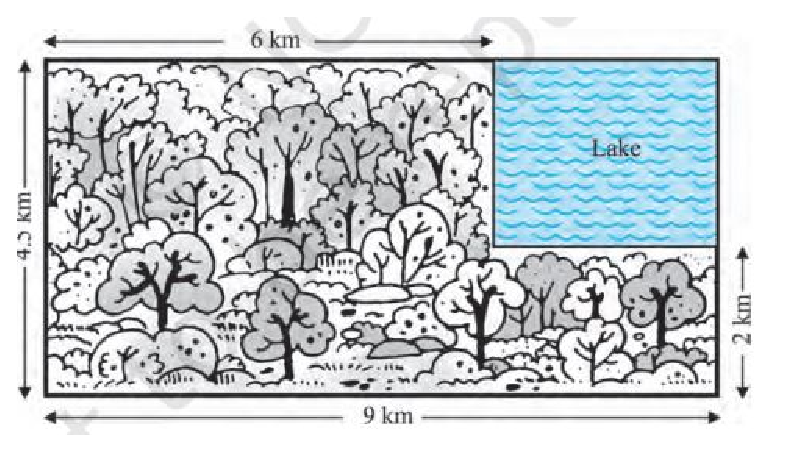
\includegraphics[width=\columnwidth]{./prob/figs/lake.eps}
\caption{}
\label{fig:lake}
\end{figure}

   \item On one page of a telephone directory, there were 200 telephone numbers.
The frequency distribution of their unit place digit (for example, in the number 25828573, the unit place digit is 3) is given in Table \ref{table:prob_exam4}
below

\begin{table}[!ht]
\centering
\resizebox{\columnwidth}{!}{
\begin{tabular}{ |c|c|c|c|c|c|c|c|c|c|c| } 
\hline
 \textbf{Digit} &0 &1 &2 &3 &4 &5 &6 &7 &8 &9 \\ 
 \hline
 \textbf{Frequency} &22 &26 &22 &22 &20 &10 &14 &28 &16 &20 \\ 
 \hline
\end{tabular}
}
\caption{}
\label{table:prob_exam4}
\end{table}
Without looking at the page, the pencil is placed on one of these numbers, i.e., the number is chosen at random. What is the probability that the digit in its unit place is 6?\\
\solution
Let X be the random variable representing the number of defective eggs from the ten eggs picked. X follows a  binomial distribution.  Since the probability of an egg being defective is 10\%, substituting n=10, p= 0.1 and k=0 in equation \eqref{eq:exam41_1}, 
probability that there is atleast one defective egg is 
\begin{align}
\pr{X \geq 1}&= 1 - \pr{X=0}  = 1-\brak{0.9}^{10}
\\
&=0.6513215599
\end{align}
The python code for the above problem is,
\begin{lstlisting}
.solutions/20-10/prob/codes/exam42.py
\end{lstlisting}


\item Suppose we throw a die once. (i) What is the probability of getting a number greater than 4 ? (ii) What is the probability of getting a number less than or
equal to 4 ?
\\
\solution
Let X be the random variable representing the number of defective eggs from the ten eggs picked. X follows a  binomial distribution.  Since the probability of an egg being defective is 10\%, substituting n=10, p= 0.1 and k=0 in equation \eqref{eq:exam41_1}, 
probability that there is atleast one defective egg is 
\begin{align}
\pr{X \geq 1}&= 1 - \pr{X=0}  = 1-\brak{0.9}^{10}
\\
&=0.6513215599
\end{align}
The python code for the above problem is,
\begin{lstlisting}
.solutions/20-10/prob/codes/exam42.py
\end{lstlisting}

\item  Given that the two numbers appearing on throwing two dice are different. Find the probability of the event `the sum of numbers on the dice is 4'.\\
\solution

	 Given the production yield per hectare of wheat of 100 farms of a village. 
		The following python code generates the required ogive.
	\begin{lstlisting}
	./solutions/20-30/codes/statistics/exercises/q25.py
	\end{lstlisting}


	
	\begin{figure}[!ht]
	\centering
	\includegraphics[width=\columnwidth]{./solutions/20-30/figs/statistics/exercises/ex_q25.eps}
	\caption{}
	\label{fig:q25_ogive}	
	\end{figure}
	
	\begin{table}[ht]
	%\begin{center}
    	%%%%%%%%%%%%%%%%%%%%%%%%%%%%%%%%%%%%%%%%%%%%%%%%%%%%%%%%%%%%%%%%%%%%%%
%%                                                                  %%
%%  This is the header of a LaTeX2e file exported from Gnumeric.    %%
%%                                                                  %%
%%  This file can be compiled as it stands or included in another   %%
%%  LaTeX document. The table is based on the longtable package so  %%
%%  the longtable options (headers, footers...) can be set in the   %%
%%  preamble section below (see PRAMBLE).                           %%
%%                                                                  %%
%%  To include the file in another, the following two lines must be %%
%%  in the including file:                                          %%
%%        \def\inputGnumericTable{}                                 %%
%%  at the beginning of the file and:                               %%
%%        \input{name-of-this-file.tex}                             %%
%%  where the table is to be placed. Note also that the including   %%
%%  file must use the following packages for the table to be        %%
%%  rendered correctly:                                             %%
%%    \usepackage[latin1]{inputenc}                                 %%
%%    \usepackage{color}                                            %%
%%    \usepackage{array}                                            %%
%%    \usepackage{longtable}                                        %%
%%    \usepackage{calc}                                             %%
%%    \usepackage{multirow}                                         %%
%%    \usepackage{hhline}                                           %%
%%    \usepackage{ifthen}                                           %%
%%  optionally (for landscape tables embedded in another document): %%
%%    \usepackage{lscape}                                           %%
%%                                                                  %%
%%%%%%%%%%%%%%%%%%%%%%%%%%%%%%%%%%%%%%%%%%%%%%%%%%%%%%%%%%%%%%%%%%%%%%



%%  This section checks if we are begin input into another file or  %%
%%  the file will be compiled alone. First use a macro taken from   %%
%%  the TeXbook ex 7.7 (suggestion of Han-Wen Nienhuys).            %%
\def\ifundefined#1{\expandafter\ifx\csname#1\endcsname\relax}


%%  Check for the \def token for inputed files. If it is not        %%
%%  defined, the file will be processed as a standalone and the     %%
%%  preamble will be used.                                          %%
\ifundefined{inputGnumericTable}

%%  We must be able to close or not the document at the end.        %%
	\def\gnumericTableEnd{\end{document}}


%%%%%%%%%%%%%%%%%%%%%%%%%%%%%%%%%%%%%%%%%%%%%%%%%%%%%%%%%%%%%%%%%%%%%%
%%                                                                  %%
%%  This is the PREAMBLE. Change these values to get the right      %%
%%  paper size and other niceties.                                  %%
%%                                                                  %%
%%%%%%%%%%%%%%%%%%%%%%%%%%%%%%%%%%%%%%%%%%%%%%%%%%%%%%%%%%%%%%%%%%%%%%

	\documentclass[12pt%
			  %,landscape%
                    ]{report}
       \usepackage[latin1]{inputenc}
       \usepackage{fullpage}
       \usepackage{color}
       \usepackage{array}
       \usepackage{longtable}
       \usepackage{calc}
       \usepackage{multirow}
       \usepackage{hhline}
       \usepackage{ifthen}

	\begin{document}


%%  End of the preamble for the standalone. The next section is for %%
%%  documents which are included into other LaTeX2e files.          %%
\else

%%  We are not a stand alone document. For a regular table, we will %%
%%  have no preamble and only define the closing to mean nothing.   %%
    \def\gnumericTableEnd{}

%%  If we want landscape mode in an embedded document, comment out  %%
%%  the line above and uncomment the two below. The table will      %%
%%  begin on a new page and run in landscape mode.                  %%
%       \def\gnumericTableEnd{\end{landscape}}
%       \begin{landscape}


%%  End of the else clause for this file being \input.              %%
\fi

%%%%%%%%%%%%%%%%%%%%%%%%%%%%%%%%%%%%%%%%%%%%%%%%%%%%%%%%%%%%%%%%%%%%%%
%%                                                                  %%
%%  The rest is the gnumeric table, except for the closing          %%
%%  statement. Changes below will alter the table's appearance.     %%
%%                                                                  %%
%%%%%%%%%%%%%%%%%%%%%%%%%%%%%%%%%%%%%%%%%%%%%%%%%%%%%%%%%%%%%%%%%%%%%%

\providecommand{\gnumericmathit}[1]{#1} 
%%  Uncomment the next line if you would like your numbers to be in %%
%%  italics if they are italizised in the gnumeric table.           %%
%\renewcommand{\gnumericmathit}[1]{\mathit{#1}}
\providecommand{\gnumericPB}[1]%
{\let\gnumericTemp=\\#1\let\\=\gnumericTemp\hspace{0pt}}
 \ifundefined{gnumericTableWidthDefined}
        \newlength{\gnumericTableWidth}
        \newlength{\gnumericTableWidthComplete}
        \newlength{\gnumericMultiRowLength}
        \global\def\gnumericTableWidthDefined{}
 \fi
%% The following setting protects this code from babel shorthands.  %%
 \ifthenelse{\isundefined{\languageshorthands}}{}{\languageshorthands{english}}
%%  The default table format retains the relative column widths of  %%
%%  gnumeric. They can easily be changed to c, r or l. In that case %%
%%  you may want to comment out the next line and uncomment the one %%
%%  thereafter                                                      %%
\providecommand\gnumbox{\makebox[0pt]}
%%\providecommand\gnumbox[1][]{\makebox}

%% to adjust positions in multirow situations                       %%
\setlength{\bigstrutjot}{\jot}
\setlength{\extrarowheight}{\doublerulesep}

%%  The \setlongtables command keeps column widths the same across  %%
%%  pages. Simply comment out next line for varying column widths.  %%
\setlongtables

\setlength\gnumericTableWidth{%
	77pt+%
	53pt+%
	53pt+%
0pt}
\def\gumericNumCols{3}
\setlength\gnumericTableWidthComplete{\gnumericTableWidth+%
         \tabcolsep*\gumericNumCols*2+\arrayrulewidth*\gumericNumCols}
\ifthenelse{\lengthtest{\gnumericTableWidthComplete > \linewidth}}%
         {\def\gnumericScale{\ratio{\linewidth-%
                        \tabcolsep*\gumericNumCols*2-%
                        \arrayrulewidth*\gumericNumCols}%
{\gnumericTableWidth}}}%
{\def\gnumericScale{1}}

%%%%%%%%%%%%%%%%%%%%%%%%%%%%%%%%%%%%%%%%%%%%%%%%%%%%%%%%%%%%%%%%%%%%%%
%%                                                                  %%
%% The following are the widths of the various columns. We are      %%
%% defining them here because then they are easier to change.       %%
%% Depending on the cell formats we may use them more than once.    %%
%%                                                                  %%
%%%%%%%%%%%%%%%%%%%%%%%%%%%%%%%%%%%%%%%%%%%%%%%%%%%%%%%%%%%%%%%%%%%%%%

\ifthenelse{\isundefined{\gnumericColA}}{\newlength{\gnumericColA}}{}\settowidth{\gnumericColA}{\begin{tabular}{@{}p{77pt*\gnumericScale}@{}}x\end{tabular}}
\ifthenelse{\isundefined{\gnumericColB}}{\newlength{\gnumericColB}}{}\settowidth{\gnumericColB}{\begin{tabular}{@{}p{53pt*\gnumericScale}@{}}x\end{tabular}}
\ifthenelse{\isundefined{\gnumericColC}}{\newlength{\gnumericColC}}{}\settowidth{\gnumericColC}{\begin{tabular}{@{}p{53pt*\gnumericScale}@{}}x\end{tabular}}

\begin{tabular}[c]{%
	b{\gnumericColA}%
	b{\gnumericColB}%
	b{\gnumericColC}%
	}

%%%%%%%%%%%%%%%%%%%%%%%%%%%%%%%%%%%%%%%%%%%%%%%%%%%%%%%%%%%%%%%%%%%%%%
%%  The longtable options. (Caption, headers... see Goosens, p.124) %%
%	\caption{The Table Caption.}             \\	%
% \hline	% Across the top of the table.
%%  The rest of these options are table rows which are placed on    %%
%%  the first, last or every page. Use \multicolumn if you want.    %%

%%  Header for the first page.                                      %%
%	\multicolumn{3}{c}{The First Header} \\ \hline 
%	\multicolumn{1}{c}{colTag}	%Column 1
%	&\multicolumn{1}{c}{colTag}	%Column 2
%	&\multicolumn{1}{c}{colTag}	\\ \hline %Last column
%	\endfirsthead

%%  The running header definition.                                  %%
%	\hline
%	\multicolumn{3}{l}{\ldots\small\slshape continued} \\ \hline
%	\multicolumn{1}{c}{colTag}	%Column 1
%	&\multicolumn{1}{c}{colTag}	%Column 2
%	&\multicolumn{1}{c}{colTag}	\\ \hline %Last column
%	\endhead

%%  The running footer definition.                                  %%
%	\hline
%	\multicolumn{3}{r}{\small\slshape continued\ldots} \\
%	\endfoot

%%  The ending footer definition.                                   %%
%	\multicolumn{3}{c}{That's all folks} \\ \hline 
%	\endlastfoot
%%%%%%%%%%%%%%%%%%%%%%%%%%%%%%%%%%%%%%%%%%%%%%%%%%%%%%%%%%%%%%%%%%%%%%

\hhline{|-|-~}
	 \multicolumn{1}{|p{\gnumericColA}|}%
	{\gnumericPB{\raggedright}\gnumbox[l]{Prodn.yield}}
	&\multicolumn{1}{p{\gnumericColB}|}%
	{\gnumericPB{\raggedright}\gnumbox[l]{No.of.farms}}
	&
\\
\hhline{|--|~}
	 \multicolumn{1}{|p{\gnumericColA}|}%
	{\gnumericPB{\raggedright}\gnumbox[l]{More than 50}}
	&\multicolumn{1}{p{\gnumericColB}|}%
	{\gnumericPB{\raggedright}\gnumbox[l]{100}}
	&
\\
\hhline{|--|~}
	 \multicolumn{1}{|p{\gnumericColA}|}%
	{\gnumericPB{\raggedright}\gnumbox[l]{More than 55}}
	&\multicolumn{1}{p{\gnumericColB}|}%
	{\gnumericPB{\raggedright}\gnumbox[l]{100-2=98}}
	&
\\
\hhline{|--|~}
	 \multicolumn{1}{|p{\gnumericColA}|}%
	{\gnumericPB{\raggedright}\gnumbox[l]{More than 60}}
	&\multicolumn{1}{p{\gnumericColB}|}%
	{\gnumericPB{\raggedright}\gnumbox[l]{98-8=90}}
	&
\\
\hhline{|--|~}
	 \multicolumn{1}{|p{\gnumericColA}|}%
	{\gnumericPB{\raggedright}\gnumbox[l]{More than 65}}
	&\multicolumn{1}{p{\gnumericColB}|}%
	{\gnumericPB{\raggedright}\gnumbox[l]{90-12=78}}
	&
\\
\hhline{|--|~}
	 \multicolumn{1}{|p{\gnumericColA}|}%
	{\gnumericPB{\raggedright}\gnumbox[l]{More than 70}}
	&\multicolumn{1}{p{\gnumericColB}|}%
	{\gnumericPB{\raggedright}\gnumbox[l]{78-24=54}}
	&
\\
\hhline{|--|~}
	 \multicolumn{1}{|p{\gnumericColA}|}%
	{\gnumericPB{\raggedright}\gnumbox[l]{More than 75}}
	&\multicolumn{1}{p{\gnumericColB}|}%
	{\gnumericPB{\raggedright}\gnumbox[l]{54-38=16}}
	&
\\
\hhline{|-|-|~}
\end{tabular}

\ifthenelse{\isundefined{\languageshorthands}}{}{\languageshorthands{\languagename}}
\gnumericTableEnd

	\caption{production yield using more than cumulative frequency}
	\label{table:stat_ex_q25anstable4}
	%\end{center}
	\end{table}




\item A game of chance consists of spinning an arrow which comes to rest pointing at one of the numbers 1, 2, 3, 4, 5, 6, 7, 8 (see Fig. \ref{fig:122} ), and these are equally likely outcomes. What is the probability that it will point at\\
(i) 8 ?\\
(ii) an odd number?\\
(iii) a number greater than 2?\\
(iv) a number less than 9?\\
\begin{figure}[!ht]
\centering
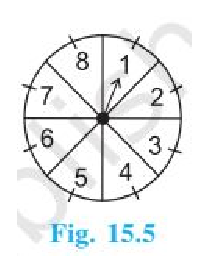
\includegraphics[width=\columnwidth]{./prob/figs/clock.eps}
\caption{}
\label{fig:122}
\end{figure}
\\
\solution
Let X be the random variable representing the number of defective eggs from the ten eggs picked. X follows a  binomial distribution.  Since the probability of an egg being defective is 10\%, substituting n=10, p= 0.1 and k=0 in equation \eqref{eq:exam41_1}, 
probability that there is atleast one defective egg is 
\begin{align}
\pr{X \geq 1}&= 1 - \pr{X=0}  = 1-\brak{0.9}^{10}
\\
&=0.6513215599
\end{align}
The python code for the above problem is,
\begin{lstlisting}
.solutions/20-10/prob/codes/exam42.py
\end{lstlisting}

\end{enumerate}


 
\section{Miscellaneous Distributions}
\renewcommand{\theequation}{\theenumi}
\begin{enumerate}[label=\thesection.\arabic*.,ref=\thesection.\theenumi]
\numberwithin{equation}{enumi}

\item It is given that in a group of 3 students, the probability of 2 students not having the
same birthday is 0.992. What is the probability that the 2 students have the same
birthday?
\\
\solution 
We know that two students either have birthday on same date or they don't have same birthday. No other cases are possible.\\
Therefore, we can consider this as a bernoulli distribution, by defining a random variable X such that,if $X=0$, then they don't have same birthday, if $X=1$, then they have same birthday.
Therefore,
\begin{align}
Pr(X=0)+Pr(X=1)=1\\
Pr(X=0)=0.992\\
Pr(X=1)=1-Pr(X=0)\\
Pr(X=0)=1-0.992\\
Pr(X=0)=0.008
\end{align}
\item 


\item A box contains 5 red marbles, 8 white marbles and 4 green marbles. One marble is taken
out of the box at random. What is the probability that the marble taken out will be\\
(i) red ?\\
(ii) white ? \\
(iii) not green?
\\
\solution 
Total number of marbles = 5 + 8 + 4 = 17 marbles.
Let $X \in \{0,1,2\}$ represent the random variable, where 0 represents a red marble, 1 represents a white marble, and 2 represents a green marble. From the given information, 
\begin{align}
    Pr(X=0) &= \frac{5}{17} \\
    Pr(X=1) &= \frac{8}{17} \\
    Pr(X=2) &= \frac{4}{17} \implies \pr{X\ne 2} = \frac{13}{17}
\end{align}

\item A piggy bank contains hundred 50p coins, fifty rupee 1 coins, twenty rupee 2 coins and ten rupee 5 coins. If it is equally likely that one of the coins will fall out when the bank is turned upside down, what is the probability that the coin \\
(i) will be a 50 p coin ?\\
(ii) will not be a rupee5 coin?\item If each element of a second order determinant is either zero or one, what is the
probability that the value of the determinant is positive? (Assume that the individual entries of the determinant are chosen independently, each value being
assumed with probability $\frac{1}{2}$).\\
\item If a leap year is selected at random, what is the chance that it will contain 53
Tuesdays?\\
\item
\item
\item Suppose that two cards are drawn at random from a deck of cards. Let X be the number of aces obtained. Then the value of E(X) is\\
\begin{enumerate}
\item $\frac{37}{221}$
\item $\frac{5}{13}$
\item $\frac{1}{13}$
\item $\frac{2}{13}$
\end{enumerate}
\item The mean of the numbers obtained on throwing a die having written 1 on three faces, 2 on two faces and 5 on one face is\\
\begin{enumerate}
\item 1
\item 2
\item 5
\item $\frac{8}{3}$
\end{enumerate}
\item A class has 15 students whose ages are 14, 17, 15, 14, 21, 17, 19, 20, 16, 18, 20,
17, 16, 19 and 20 years. One student is selected in such a manner that each has the same chance of being chosen and the age X of the selected student is recorded. What is the probability distribution of the random variable X? Find mean, variance and standard deviation of X.\\
\solution  Table \ref{table:5.11} summarizes the given info.
\begin{table}[!ht]
\begin{center}
\begin{tabular}{|c|c|c|c|c|c|c|c|c|}
\hline
{X} & 0 & 1 & 2 & 3 & 4 & 5 & 6 & 7 \\
\hline
{No. of students} & 2 & 1 & 2 & 3 & 1 & 2 & 3 & 1 \\
\hline
{P(X)} & $\frac {2}{15}$ & $\frac {1}{15}$ & $\frac {2}{15}$ & $\frac {3}{15}$ & $\frac {1}{15}$ & $\frac {2}{15}$ & $\frac {3}{15}$ & $\frac {1}{15}$
\\
\hline 
\end{tabular}
\end{center}
\caption{}
\label{table:5.11}
\end{table}
using which, 
 \begin{align}
      E(X) &= \sum_{i=1}^n x_i \pr{X=i} = \frac{263}{15}
      \\
    E(X^2) = \sum_{i=1}^n x_i^2 \pr{X=i} =    \frac{4683}{15}
    \\
    \implies Var (X) = \frac{4683}{15} - (\frac{263}{15})^2
    = 4.78
    \end{align}
\item A random variable X has the following probability distribution:\\
\\$\begin{tabular}{||c c c c c c c c c||} 
 \hline
 X & 0 & 1 & 2 & 3 & 4 & 5 & 6 & 7 \\
 \hline
 P(X) & 0 & k & 2k & 2k & 3k & $k^2$ & 2$k^2$ & 7$k^2$+k \\
 \hline
\end{tabular}$\\
\\Determine\\
(i) k \\
(ii) P(X < 3)\\
(iii) P(X > 6)\\
(iv) P(0 < X < 3)\\\item Find the probability distribution of the number of successes in two tosses of a die, where a success is defined as\\
(i) number greater than 4\\
(ii) six appears on at least one die\\
\item An urn contains 5 red and 2 black balls. Two balls are randomly drawn. Let X represent the number of black balls. What are the possible values of X? Is X a random variable ?\\
\item State which of the following are not the probability distributions of a random variable. Give reasons for your answer.\\
(i) \\$\begin{tabular}{||c c c c||} 
 \hline
 X & 0 & 1 & 2 \\
 \hline
 P(X) & 0.4 & 0.4 & 0.2 \\
 \hline
\end{tabular}$\\

(ii) \\$\begin{tabular}{||c c c c c c||} 
 \hline
 X & 0 & 1 & 2 & 3 & 4 \\
 \hline
 P(X) & 0.1 & 0.5 & 0.2 & -0.1 & 0.3 \\
 \hline
\end{tabular}$\\

(iii) \\$\begin{tabular}{||c c c c||} 
 \hline
 X & -1 & 0 & 1 \\
 \hline
 P(X) & 0.6 & 0.1 & 0.2 \\
 \hline
\end{tabular}$\\

(iv) \\$\begin{tabular}{||c c c c c c||} 
 \hline
 X & 3 & 2 & 1 & 0 & -1 \\
 \hline
 P(X) & 0.3 & 0.2 & 0.4 & 0.1 & 0.05 \\
 \hline
\end{tabular}$\\
\solution Only (i) is valid.  The remaining do not satisfy one of the following 
conditions.
\begin{align}
0 \le \pr{X = i} \le 1
\\
\sum_{i}\pr{X=i} = 1
\end{align}
\item A card from a pack of 52 cards is lost. From the remaining cards of the pack, two cards are drawn and are found to be both diamonds. Find the probability of the lost card being a diamond.\\
\item Suppose a girl throws a die. If she gets a 5 or 6, she tosses a coin three times and notes the number of heads. If she gets 1, 2, 3 or 4, she tosses a coin once and notes whether a head or tail is obtained. If she obtained exactly one head, what is the probability that she threw 1, 2, 3 or 4 with the die?\\
\solution 
Let $X\in\{0,1\}$ where X=0 represents that we get 1,2,3 or 4 when a die is rolled and X=1 represents that we get 5 or 6 when a die is rolled. \\
Let $Y\in\{0,1,2,3\}$ where Y=1 represents that we get exactly one head.Here Y represents the number of heads obtained. \\ 

We are required to find probability of getting X=0 when Y=1.\\
Here we use Bayes' theorem.

\begin{equation}
   \pr{X=0|Y=1}= \frac{\pr{X=0} \hspace{0.2cm} \pr{Y=1|X=0}}{\sum\limits_{i=0}^{1} \pr{X=i} \hspace{0.2cm} \pr{Y=1|X=i}}
\end{equation} 

Note that 
\begin{align}
    \pr{X=0} = \frac{4}{6} = \frac{2}{3} = 0.6666666667 \\
    \pr{X=1} = \frac{2}{6} = \frac{1}{3} = 0.3333333333
\end{align} 

Also we get
\begin{align}
    \pr{Y=1|X=0} = \frac{1}{2} = 0.5 \\
    \pr{Y=1|X=1} = \frac{3}{8} = 0.375
\end{align} 

Substituting values, we get
\begin{align}
    \pr{X=0|Y=1} = \frac{\frac{2}{3} \times \frac{1}{2}}{{\frac{2}{3} \times \frac{1}{2}} + \frac{1}{3} \times \frac{3}{8}} \\
\implies \pr{X=0|Y=1} = \frac{8}{11} = 0.7272727273
\end{align} 

\item An insurance company insured 2000 scooter drivers, 4000 car drivers and 6000 truck drivers. The probability of an accidents are 0.01, 0.03 and 0.15 respectively. One of the insured persons meets with an accident. What is the probability that he is a scooter driver?\\
\solution 
By definition
\begin{align}
\pr{A|B} = \frac{\pr{AB}}{\pr{B}} \label{5.18:1}
\end{align}
Also, by Bayes' Theorem
\begin{align}
\pr{A} = \sum_{i=1}^n \pr{A|E_i}\pr{E_i}\label{5.18:2}
\end{align}
where $E_1 , E_2 \ldots E_n$  are partitions of the complete sample set.\\

Let X be a random variable taking the following values in Table \ref{table:5.18}.
\begin{table}[!ht]
\begin{center}
\begin{tabular}{ |c|c| } 
 \hline
 X = 0 & Scooter Drivers\\
 \hline
 X = 1 & Car Drivers\\
 \hline
X = 2 & Truck Drivers\\
 \hline
\end{tabular}
\end{center}
\caption{}
\label{table:5.18}
\end{table}
where X $\in \{0, 1, 2\}$ represent all the partitions of the sample set.


Let Y be a random variable taking the following values in Table \ref{table:5.18_1}.
\begin{table}[!ht]
\begin{center}
\begin{tabular}{ |c|c| } 
 \hline
 Y = 0 & Involved in an accident\\
 \hline
 Y = 1 & Not involved in an accident\\
 \hline
\end{tabular}
\end{center}
\caption{}
\label{table:5.18_1}
\end{table}

 Also, the following values are known:
\begin{align}
\pr{X = 0} = \frac{2000}{2000+4000+6000} = \frac{1}{6}\\
\pr{X = 1} = \frac{4000}{2000+4000+6000} = \frac{1}{3}\\
\pr{X = 2} = \frac{6000}{2000+4000+6000} = \frac{1}{2}\\
\pr{Y = 0|X = 0} = 0.01\\
\pr{Y = 0|X = 1} = 0.03\\
\pr{Y = 0|X = 2} = 0.15
\end{align}

We have to find:
\begin{align}
\pr{X = 0|Y = 0} = \frac{\pr{X = 0 \cap Y = 0}}{\pr{Y = 0}}
\end{align}
Using \eqref{1} and \eqref{2}, we get:
\begin{multline}
\pr{X = 0|Y = 0} 
\\
= \frac{\pr{Y = 0|X = 0}\pr{X = 0}}{\sum_{i=0}^{i=2}\pr{Y = 0 | X = i}\pr{X = i}}
\\
= \frac{\frac{0.01}{6}}{\frac{0.01}{6} + \frac{0.03}{3} + \frac{0.15}{2}}
 = \frac{1}{52}
\end{multline}

\item A carton consists of 100 shirts of which 88 are good, 8 have minor defects and 4 have major defects.Jimmy, a trader, will only accept the shirts which are good, but Sujatha, another trader, will only reject the shirts which have major defects.One shirt is drawn at random from the carton. What is the probability that\\
(i) it is acceptable to Jimmy?\\
(ii) it is acceptable to Sujatha?
\\
\solution
Let random variable  $X\in\{0,1,2\}$ denote the outcomes of experiment of drawing a shirt from the carton as shown in Table \ref{table:}
\begin{table}[h]
\centering 
\caption{}
\begin{tabular}{|c|c|c|c|}
\hline
Type of shirt & X & number      & \pr{X}      \\
\hline
good          & 0 & n(X=0) = 88 & $\frac{22}{25}$ \\
\hline
minor defect  & 1 & n(X=1) = 8  & $\frac{2}{25}$ \\
\hline
major defect  & 2 & n(X=2) = 4  & $\frac{1}{25}$\\
\hline
\end{tabular}
\label{table:}
\end{table}

\begin{enumerate}[label={\roman*)}]
    \item The required probability is
    \begin{align}
      p &= \pr{X=0}\\
        &= \frac{88}{100}\\
        &= 0.88
    \end{align}
    \item The required probability is
    \begin{align}
        p &= \pr{X=0}+\pr{X=1}\\
          &= \frac{88}{100}+\frac{8}{100}\\
          &=0.96
    \end{align}
\end{enumerate}
\item Two dice, one blue and one grey, are thrown at the same time. Write down all the possible outcomes.What is the probability that the sum of the two numbers appearing on the top of the dice is\\
(i) 8?\\
(ii) 13?\\ 
(iii) less than or equal to 12?\\\\
\item Savita and Hamida are friends. What is the probability that both will have \\
(i) different birthdays? \\
(ii) the same birthday? (ignoring a leap year).
\item 
\item  A box contains 3 blue, 2 white, and 4 red marbles. If a marble is drawn
at random from the box, what is the probability that it will be
(i) white? (ii) blue? (iii) red?
\\
\solution 
Consider the random variable X = \{0,1,2\} represent the marble colour blue or white or red.\\
\begin{table}[ht]
\begin{tabular}{|c|c|c|c|}
\hline
\textbf{Color}&\textbf{X}&\textbf{N(X)}&\textbf{Pr(X)}  \\ \hline    
Blue  &0  &3  &3/9  \\ \hline
White  &1  &2  &2/9  \\ \hline
Red  &2  &4  &4/9  \\ \hline
\end{tabular}
\caption{Table for probabilities of marbles}
\label{table:data}
\end{table}
Picking up any marble from the box is equally - likely.
The box contain a total of 9 marbles.

\begin{align}
 \pr{X=0} = \frac{N(X=0)}{9} = \frac{3}{9}\\
 \pr{X=1} = \frac{N(X=1)}{9} = \frac{2}{9}\\
 \pr{X=2} = \frac{N(X=2)}{9} = \frac{4}{9}
\end{align}

\item One card is drawn from a well-shuffled deck of 52 cards. Calculate the
probability that the card will\\
(i) be an ace,\\
(ii) not be an ace.
\\
\solution 
For convinience, let's denote the cards Ace, J, Q, K by the numbers $\{ 1, 11, 12, 13\}$ respectively. Let $X \in \{ 1, 2, 3, 4, 5, 6, 7, 8, 9, 10, 11, 12, 13 \}$ denote the outcome of the experiment. We know that there exist exactly 4 cards with a particular number in a deck of 52 cards. Assuming that the deck of cards is well-shuffled, the probability mass function for this experiment is expressed as\\
\begin{align}
	\Pr(X=i) = 
	\begin{cases}
	\dfrac{4}{52} = \dfrac{1}{13} & 1 \leq i \leq 13, \; i \in \mathbb{N}\\ ~\\[-1em]
	0 & \text{otherwise}
	\end{cases}
\end{align}
\begin{enumerate}[label = (\roman*)]
\item Hence, the probability of getting an Ace is 
\begin{align}
	\Pr(X=1) = \dfrac{1}{13} 
\end{align}
\item Hence, the probability of not getting an Ace is
\begin{align}
	\Pr(X \neq 1) &= \sum_{i=2} ^{13} \Pr(X=i) \\
	&= 1 - \Pr(X=1) \\
	&= 1 - \dfrac{1}{13} \\
	&= \dfrac{12}{13}
\end{align}
\end{enumerate}
\item 
\item Two cards are drawn successively with replacement from a well shuffled deck of 52 cards. Find the probability distribution of the number of aces.\\

\item Find the probability distribution of number of doublets in three throws of a pair of dice?\\

\item Let X denote the number of hours you study during a randomly selected school day. The probability that X can take the values x, has the following form, where k is some unknown constant.\\
\begin{align}
    P\brak{X=x} =
    \begin{cases}
      0.1, & \text{if}\ x=0 \\
      kx,  & \text{if}\ x= 1 \; \text{or}\ 2 \\
      k(5-x) & \text{if}\ x= 3 \; \text{or}\ 4 \\
      0, & \text{otherwise}
    \end{cases}
  \end{align}
%P(X=x)= $\begin{pmatrix} 0.1, if x= 0 \\ kx,if x= 1 or 2 \\ k(5-x), if x= 3 or 4 \\ 0, otherwise \end{pmatrix}$
\begin{enumerate}
\item  Find the value of k.
\item  What is the probability that you study at least two hours ? Exactly two hours? At
most two hours?
\end{enumerate}
\solution
\begin{enumerate}
\item 
\begin{align}
    \because & \quad \sum_{x=0}^4 P(X=x) = 1,\\
    & 0.1 + k +2k +2k +k = 1\\
    &\implies 0.1 +6k = 1\\
    &\implies k = 0.15
\end{align}
\item 
Probability of studying atleast 2 hours
\begin{align}
    &= P\brak{X\ge 2}\\
    &=\sum_{x=2}^4 P(X=x)\\
    &= P(X=2)+ P(X=3) +P(X=4)\\
    &= 2k + 2k +k\\
    &= 5 \times 0.15\\
    &= 0.75
\end{align}
Probability of studying exactly 2 hours
\begin{align}
    &=P(X=2)\\
    &= 0.15 \times 2\\
    &= 0.30
\end{align}
Probability of studying atmost 2 hours
\begin{align}
    &= P\brak{X\le 2}\\ 
    &=\sum_{x=0}^2 P(X=x)\\
    &= P(X=0) + P(X=1)+ P(X=2)\\
    &= 0.1 + 0.15 +0.30\\
    &=0.55
\end{align}
\end{enumerate}

\item Let a pair of dice be thrown and the random variable X be the sum of the numbers that appear on the two dice. Find the mean or expectation of X.\\

\item

\item Two cards are drawn simultaneously (or successively without replacement) from a well shuffled pack of 52 cards. Find the mean, variance and standard deviation of the number of kings.\\
\solution
Let $X \cbrak{ 0, 1, 2 }$ be the  random variable representing the number of kings present in the two cards.
%
Then,
%
\begin{align}
\pr{X=0} &= \frac{\comb{48}{2}}{\comb{52}{2}} = \frac{188}{221} 
\\
\pr{X=1} &= \frac{\comb{4}{1} \times \comb{48}{1}}{\comb{52}{2}} = \frac{32}{221} 
\\
\pr{X=2} &= \frac{\comb{4}{2}}{\comb{52}{2}} = \frac{1}{221}
\end{align}
and
\begin{align}
E(X) &= \sum_{i=0}^{2} i\pr{X=i} 
\\
&= 0\times\frac{188}{221} + \frac{32}{221} + 2\times\frac{1}{221}
\\
&= \frac{36}{221}
\end{align}
Similarly,
%
\begin{align}
E\brak{X^2} &= \sum_{i=0}^{2} i^2\pr{X=i} = \frac{34}{221}
\\
\implies Var\brak{X}&=  E\brak{X^2} - \brak{E\brak{X} }^2 = \frac{6800}{48841}
\end{align}
\item A tyre manufacturing company kept a record of the distance covered
before a tyre needed to be replaced. Table \ref{table:prob_exam6}
shows the results of 1000 cases.
\begin{table}[!ht]
\centering
\resizebox{\columnwidth}{!}{
\begin{tabular}{ |c|c|c|c|c| } 
 \hline
 \textbf{Distance(in km)} &$>$ 4000 &4000-9000 &9001-14000 &$<$14000 \\ 
 \hline
 \textbf{Frequency} &20 &210 &325 &445\\ 
 \hline
\end{tabular}
}
\caption{}
\label{table:prob_exam6}
\end{table}
If you buy a tyre of this company, what is the probability that :\\
(i) it will need to be replaced before it has covered 4000 km?\\
(ii) it will last more than 9000 km?\\
(iii) it will need to be replaced after it has covered somewhere between 4000 km and 14000 km?\\
\solution
See Table \ref{table:2.1.6.sol}.
 \begin{table}[!ht]
	\centering
	%%%%%%%%%%%%%%%%%%%%%%%%%%%%%%%%%%%%%%%%%%%%%%%%%%%%%%%%%%%%%%%%%%%%%%
%%                                                                  %%
%%  This is the header of a LaTeX2e file exported from Gnumeric.    %%
%%                                                                  %%
%%  This file can be compiled as it stands or included in another   %%
%%  LaTeX document. The table is based on the longtable package so  %%
%%  the longtable options (headers, footers...) can be set in the   %%
%%  preamble section below (see PRAMBLE).                           %%
%%                                                                  %%
%%  To include the file in another, the following two lines must be %%
%%  in the including file:                                          %%
%%        \def\inputGnumericTable{}                                 %%
%%  at the beginning of the file and:                               %%
%%        \input{name-of-this-file.tex}                             %%
%%  where the table is to be placed. Note also that the including   %%
%%  file must use the following packages for the table to be        %%
%%  rendered correctly:                                             %%
%%    \usepackage[latin1]{inputenc}                                 %%
%%    \usepackage{color}                                            %%
%%    \usepackage{array}                                            %%
%%    \usepackage{longtable}                                        %%
%%    \usepackage{calc}                                             %%
%%    \usepackage{multirow}                                         %%
%%    \usepackage{hhline}                                           %%
%%    \usepackage{ifthen}                                           %%
%%  optionally (for landscape tables embedded in another document): %%
%%    \usepackage{lscape}                                           %%
%%                                                                  %%
%%%%%%%%%%%%%%%%%%%%%%%%%%%%%%%%%%%%%%%%%%%%%%%%%%%%%%%%%%%%%%%%%%%%%%



%%  This section checks if we are begin input into another file or  %%
%%  the file will be compiled alone. First use a macro taken from   %%
%%  the TeXbook ex 7.7 (suggestion of Han-Wen Nienhuys).            %%
\def\ifundefined#1{\expandafter\ifx\csname#1\endcsname\relax}


%%  Check for the \def token for inputed files. If it is not        %%
%%  defined, the file will be processed as a standalone and the     %%
%%  preamble will be used.                                          %%
\ifundefined{inputGnumericTable}

%%  We must be able to close or not the document at the end.        %%
	\def\gnumericTableEnd{\end{document}}


%%%%%%%%%%%%%%%%%%%%%%%%%%%%%%%%%%%%%%%%%%%%%%%%%%%%%%%%%%%%%%%%%%%%%%
%%                                                                  %%
%%  This is the PREAMBLE. Change these values to get the right      %%
%%  paper size and other niceties.                                  %%
%%                                                                  %%
%%%%%%%%%%%%%%%%%%%%%%%%%%%%%%%%%%%%%%%%%%%%%%%%%%%%%%%%%%%%%%%%%%%%%%

	\documentclass[12pt%
			  %,landscape%
                    ]{report}
       \usepackage[latin1]{inputenc}
       \usepackage{fullpage}
       \usepackage{color}
       \usepackage{array}
       \usepackage{longtable}
       \usepackage{calc}
       \usepackage{multirow}
       \usepackage{hhline}
       \usepackage{ifthen}

	\begin{document}


%%  End of the preamble for the standalone. The next section is for %%
%%  documents which are included into other LaTeX2e files.          %%
\else

%%  We are not a stand alone document. For a regular table, we will %%
%%  have no preamble and only define the closing to mean nothing.   %%
    \def\gnumericTableEnd{}

%%  If we want landscape mode in an embedded document, comment out  %%
%%  the line above and uncomment the two below. The table will      %%
%%  begin on a new page and run in landscape mode.                  %%
%       \def\gnumericTableEnd{\end{landscape}}
%       \begin{landscape}


%%  End of the else clause for this file being \input.              %%
\fi

%%%%%%%%%%%%%%%%%%%%%%%%%%%%%%%%%%%%%%%%%%%%%%%%%%%%%%%%%%%%%%%%%%%%%%
%%                                                                  %%
%%  The rest is the gnumeric table, except for the closing          %%
%%  statement. Changes below will alter the table's appearance.     %%
%%                                                                  %%
%%%%%%%%%%%%%%%%%%%%%%%%%%%%%%%%%%%%%%%%%%%%%%%%%%%%%%%%%%%%%%%%%%%%%%

\providecommand{\gnumericmathit}[1]{#1} 
%%  Uncomment the next line if you would like your numbers to be in %%
%%  italics if they are italizised in the gnumeric table.           %%
%\renewcommand{\gnumericmathit}[1]{\mathit{#1}}
\providecommand{\gnumericPB}[1]%
{\let\gnumericTemp=\\#1\let\\=\gnumericTemp\hspace{0pt}}
 \ifundefined{gnumericTableWidthDefined}
        \newlength{\gnumericTableWidth}
        \newlength{\gnumericTableWidthComplete}
        \newlength{\gnumericMultiRowLength}
        \global\def\gnumericTableWidthDefined{}
 \fi
%% The following setting protects this code from babel shorthands.  %%
 \ifthenelse{\isundefined{\languageshorthands}}{}{\languageshorthands{english}}
%%  The default table format retains the relative column widths of  %%
%%  gnumeric. They can easily be changed to c, r or l. In that case %%
%%  you may want to comment out the next line and uncomment the one %%
%%  thereafter                                                      %%
\providecommand\gnumbox{\makebox[0pt]}
%%\providecommand\gnumbox[1][]{\makebox}

%% to adjust positions in multirow situations                       %%
\setlength{\bigstrutjot}{\jot}
\setlength{\extrarowheight}{\doublerulesep}

%%  The \setlongtables command keeps column widths the same across  %%
%%  pages. Simply comment out next line for varying column widths.  %%
\setlongtables

\setlength\gnumericTableWidth{%
	49pt+%
	49pt+%
	53pt+%
	49pt+%
0pt}
\def\gumericNumCols{4}
\setlength\gnumericTableWidthComplete{\gnumericTableWidth+%
         \tabcolsep*\gumericNumCols*2+\arrayrulewidth*\gumericNumCols}
\ifthenelse{\lengthtest{\gnumericTableWidthComplete > \linewidth}}%
         {\def\gnumericScale{\ratio{\linewidth-%
                        \tabcolsep*\gumericNumCols*2-%
                        \arrayrulewidth*\gumericNumCols}%
{\gnumericTableWidth}}}%
{\def\gnumericScale{1}}

%%%%%%%%%%%%%%%%%%%%%%%%%%%%%%%%%%%%%%%%%%%%%%%%%%%%%%%%%%%%%%%%%%%%%%
%%                                                                  %%
%% The following are the widths of the various columns. We are      %%
%% defining them here because then they are easier to change.       %%
%% Depending on the cell formats we may use them more than once.    %%
%%                                                                  %%
%%%%%%%%%%%%%%%%%%%%%%%%%%%%%%%%%%%%%%%%%%%%%%%%%%%%%%%%%%%%%%%%%%%%%%

\ifthenelse{\isundefined{\gnumericColA}}{\newlength{\gnumericColA}}{}\settowidth{\gnumericColA}{\begin{tabular}{@{}p{49pt*\gnumericScale}@{}}x\end{tabular}}
\ifthenelse{\isundefined{\gnumericColB}}{\newlength{\gnumericColB}}{}\settowidth{\gnumericColB}{\begin{tabular}{@{}p{49pt*\gnumericScale}@{}}x\end{tabular}}
\ifthenelse{\isundefined{\gnumericColC}}{\newlength{\gnumericColC}}{}\settowidth{\gnumericColC}{\begin{tabular}{@{}p{53pt*\gnumericScale}@{}}x\end{tabular}}
\ifthenelse{\isundefined{\gnumericColD}}{\newlength{\gnumericColD}}{}\settowidth{\gnumericColD}{\begin{tabular}{@{}p{49pt*\gnumericScale}@{}}x\end{tabular}}

\resizebox{\columnwidth}{!}{
\begin{tabular}[c]{%
	b{\gnumericColA}%
	b{\gnumericColB}%
	b{\gnumericColC}%
	b{\gnumericColD}%
	}

%%%%%%%%%%%%%%%%%%%%%%%%%%%%%%%%%%%%%%%%%%%%%%%%%%%%%%%%%%%%%%%%%%%%%%
%%  The longtable options. (Caption, headers... see Goosens, p.124) %%
%	\caption{The Table Caption.}             \\	%
% \hline	% Across the top of the table.
%%  The rest of these options are table rows which are placed on    %%
%%  the first, last or every page. Use \multicolumn if you want.    %%

%%  Header for the first page.                                      %%
%	\multicolumn{4}{c}{The First Header} \\ \hline 
%	\multicolumn{1}{c}{colTag}	%Column 1
%	&\multicolumn{1}{c}{colTag}	%Column 2
%	&\multicolumn{1}{c}{colTag}	%Column 3
%	&\multicolumn{1}{c}{colTag}	\\ \hline %Last column
%	\endfirsthead

%%  The running header definition.                                  %%
%	\hline
%	\multicolumn{4}{l}{\ldots\small\slshape continued} \\ \hline
%	\multicolumn{1}{c}{colTag}	%Column 1
%	&\multicolumn{1}{c}{colTag}	%Column 2
%	&\multicolumn{1}{c}{colTag}	%Column 3
%	&\multicolumn{1}{c}{colTag}	\\ \hline %Last column
%	\endhead

%%  The running footer definition.                                  %%
%	\hline
%	\multicolumn{4}{r}{\small\slshape continued\ldots} \\
%	\endfoot

%%  The ending footer definition.                                   %%
%	\multicolumn{4}{c}{That's all folks} \\ \hline 
%	\endlastfoot
%%%%%%%%%%%%%%%%%%%%%%%%%%%%%%%%%%%%%%%%%%%%%%%%%%%%%%%%%%%%%%%%%%%%%%

\hhline{|-|-|-|-}
	 \multicolumn{1}{|p{\gnumericColA}|}%
	{\gnumericPB{\centering}Class interval}
	&\multicolumn{1}{p{\gnumericColB}|}%
	{\gnumericPB{\centering}No of student}
	&\multicolumn{1}{p{\gnumericColC}|}%
	{\gnumericPB{\raggedright}\gnumbox[l]{midpoint (x)}}
	&\multicolumn{1}{p{\gnumericColD}|}%
	{\gnumericPB{\raggedright}\gnumbox[l]{f.x}}
\\
\hhline{|----|}
	 \multicolumn{1}{|p{\gnumericColA}|}%
	{\gnumericPB{\centering}10-25}
	&\multicolumn{1}{p{\gnumericColB}|}%
	{\gnumericPB{\centering}2}
	&\multicolumn{1}{p{\gnumericColC}|}%
	{\gnumericPB{\raggedleft}\gnumbox[r]{17.5}}
	&\multicolumn{1}{p{\gnumericColD}|}%
	{\gnumericPB{\raggedleft}\gnumbox[r]{35}}
\\
\hhline{|----|}
	 \multicolumn{1}{|p{\gnumericColA}|}%
	{\gnumericPB{\centering}25-40}
	&\multicolumn{1}{p{\gnumericColB}|}%
	{\gnumericPB{\centering}3}
	&\multicolumn{1}{p{\gnumericColC}|}%
	{\gnumericPB{\raggedleft}\gnumbox[r]{32.5}}
	&\multicolumn{1}{p{\gnumericColD}|}%
	{\gnumericPB{\raggedleft}\gnumbox[r]{97.5}}
\\
\hhline{|----|}
	 \multicolumn{1}{|p{\gnumericColA}|}%
	{\gnumericPB{\centering}40-55}
	&\multicolumn{1}{p{\gnumericColB}|}%
	{\gnumericPB{\centering}7}
	&\multicolumn{1}{p{\gnumericColC}|}%
	{\gnumericPB{\raggedleft}\gnumbox[r]{47.5}}
	&\multicolumn{1}{p{\gnumericColD}|}%
	{\gnumericPB{\raggedleft}\gnumbox[r]{332.5}}
\\
\hhline{|----|}
	 \multicolumn{1}{|p{\gnumericColA}|}%
	{\gnumericPB{\centering}55-70}
	&\multicolumn{1}{p{\gnumericColB}|}%
	{\gnumericPB{\centering}6}
	&\multicolumn{1}{p{\gnumericColC}|}%
	{\gnumericPB{\raggedleft}\gnumbox[r]{62.5}}
	&\multicolumn{1}{p{\gnumericColD}|}%
	{\gnumericPB{\raggedleft}\gnumbox[r]{375}}
\\
\hhline{|----|}
	 \multicolumn{1}{|p{\gnumericColA}|}%
	{\gnumericPB{\centering}70-85}
	&\multicolumn{1}{p{\gnumericColB}|}%
	{\gnumericPB{\centering}6}
	&\multicolumn{1}{p{\gnumericColC}|}%
	{\gnumericPB{\raggedleft}\gnumbox[r]{77.5}}
	&\multicolumn{1}{p{\gnumericColD}|}%
	{\gnumericPB{\raggedleft}\gnumbox[r]{465}}
\\
\hhline{|----|}
	 \multicolumn{1}{|p{\gnumericColA}|}%
	{\gnumericPB{\centering}85-100}
	&\multicolumn{1}{p{\gnumericColB}|}%
	{\gnumericPB{\centering}6}
	&\multicolumn{1}{p{\gnumericColC}|}%
	{\gnumericPB{\raggedleft}\gnumbox[r]{92.5}}
	&\multicolumn{1}{p{\gnumericColD}|}%
	{\gnumericPB{\raggedleft}\gnumbox[r]{555}}
\\
\hhline{|-|-|-|-|}
\end{tabular}
}
\ifthenelse{\isundefined{\languageshorthands}}{}{\languageshorthands{\languagename}}
\gnumericTableEnd

	\caption{}
\label{table:2.1.6.sol}
\end{table}
In this table max friquency is 8 and modal class related to it is 3-5.
\\
\begin{align}
l &= 40
\\
h = 15
\\
f_1 &= 3
\\
f_0 &= 7
\\
f_2 &= 6
\\
Mode &= l+\frac{f_1 - f_o}{2f_1 - f_o - f_2}\times h
\\
&= 40 +\frac{7 - 3}{2\times 7 - 6- 3}\times 2
\\
&=52
\end{align}
Related code is available in 
\begin{lstlisting}
./solutions/1-10/codes/statexm/sataexm6.py
\end{lstlisting}


\item The percentage of marks obtained by a student in the monthly unit tests are given in Table \ref{table:prob_exam7}
below.
Based on this data, find the probability that the student gets more than 70$\%$ marks in a unit test.\\

\begin{table}[!ht]
\centering
\resizebox{\columnwidth}{!}{
\begin{tabular}{ |c|c|c|c|c|c| } 
 \hline
 \textbf{Unit test} &I &II &III &IV &V \\ 
 \hline
 \textbf{Frequency }&69 &71 &73 &68 &74\\ 
 \hline
\end{tabular}
}
\caption{}
\label{table:prob_exam7}
\end{table}
\solution
From the given information,
\begin{align}
\pr{X>70} &= \frac{3}{5}
\\
&= 0.6
\end{align}

\item Consider the frequency distribution in Table \ref{table:prob_exam9} below which gives the weights of 38 students of a class.
(i) Find the probability that the weight of a student in the class lies in the interval 46-50 kg.\\
(ii) Give two events in this context, one having probability 0 and the other having probability 1.

%
\begin{table}[!ht]
\centering
\resizebox{\columnwidth}{!}{
\begin{tabular}{ |c|c| } 
 \hline
 \textbf{Weights (in kg)} &\textbf{Number of students }\\ 
 \hline
 31-35 &9\\
 36-40 &5\\
 41-45 &14\\
 46-50 &3\\
 51-55 &1\\
 56-60 &2\\
 61-65 &2\\
 66-70 &1\\
 71-75 &1\\
 \hline
 \textbf{Total} &38\\
 \hline
\end{tabular}
}
\caption{}
\label{table:prob_exam9}
\end{table}
\solution
\begin{enumerate}
\item 
From the given information, 
\begin{align}
\pr{46<X<50} &= \frac{3}{38}
\\
&= 0.079
\end{align}

\item There is no student whose weight is less than 31 kg thus the probability of a student to have the weight less than 31 kg = 0\\

All of the student in this context  have the weight between 31-75 so we can say that the probability of the students to have the weight in the range 31-75 = 1
\end{enumerate}

\item Fifty seeds were selected at random from each of 5 bags of seeds, and were kept under standardised conditions favourable to germination. After 20 days, the
number of seeds which had germinated in each collection were counted and recorded in Table \ref{table:prob_exam10}

What is the probability of germination of
(i)more than 40 seeds in a bag?\\
(ii) 49 seeds in a bag?\\
(iii) more that 35 seeds in a bag?\\

\begin{table}[!ht]
\centering
\resizebox{\columnwidth}{!}{
\begin{tabular}{ |c|c|c|c|c|c| } 
 \hline
 \textbf{Bag} &1 &2 &3 &4 &5\\ 
 \hline
\textbf{No.of seeds germinated} &40 &48 &42 &39 &41 \\ 
 \hline
\end{tabular}
}
\caption{}
\label{table:prob_exam10}
\end{table}
\solution
Let $X$ represent the seeds and $Y$ represent the bags.
\begin{enumerate}
\item 
\begin{align}
\pr{X > 40} &= \frac{3}{5}
\\
&= 0.6
\end{align}
\item
\begin{align}
\pr{X=49} &= \frac{0}{5}
\\
&= 0
\end{align}
\item 
\begin{align}
\pr{X>35} &= \frac{5}{5}
\\
&= 1
\end{align}
Related code is available in
\begin{lstlisting}
solutions/1-10/codes/probexm/probexm10.py
\end{lstlisting}
%\begin{figure}[!ht]
%	\centering
%	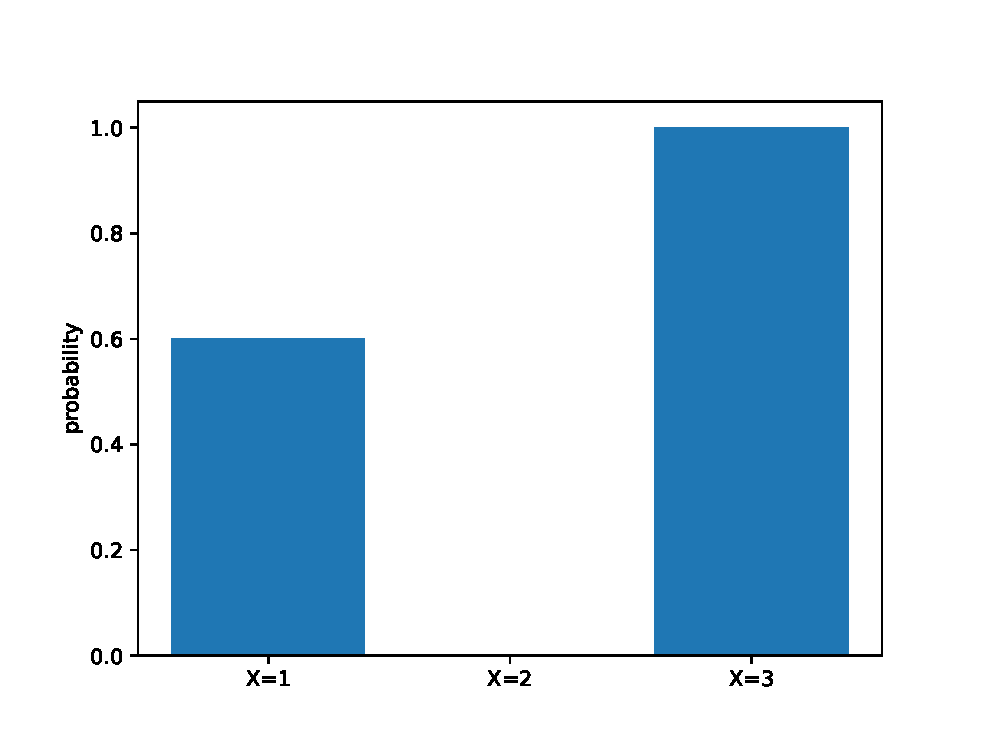
\includegraphics[width=\columnwidth]{./figures/probexm/probexm10.eps}
%	\caption{probability of germinated seeds in a bag }
%	\label{fig:bt10}
%	\begin{lstlisting}
%	figs/probexm/probexm10.eps
%	\end{lstlisting}
%\end{figure}
\end{enumerate}

    \item 1500 families with 2 children were selected randomly, and the following data in Table \ref{table:1.2.2} were recorded.
Compute the probability of a family, chosen at random, having
\begin{enumerate}
\item 2 girls
\item  1 girl
\item  No girl
\end{enumerate}
Also check whether the sum of these probabilities is 1.
\begin{table}[!ht]
\centering
\begin{tabular}{ |c|c|c|c| } 
 \hline
 \textbf{No.of girls in a family} &2 &1 &0\\ 
 \hline
 \textbf{No. of families}  &475 &814 &211\\ 
 \hline 
\end{tabular}
\caption{}
\label{table:1.2.2}
\end{table}
\\
\solution
Let X be the random variable representing the number of defective eggs from the ten eggs picked. X follows a  binomial distribution.  Since the probability of an egg being defective is 10\%, substituting n=10, p= 0.1 and k=0 in equation \eqref{eq:exam41_1}, 
probability that there is atleast one defective egg is 
\begin{align}
\pr{X \geq 1}&= 1 - \pr{X=0}  = 1-\brak{0.9}^{10}
\\
&=0.6513215599
\end{align}
The python code for the above problem is,
\begin{lstlisting}
.solutions/20-10/prob/codes/exam42.py
\end{lstlisting}


\item In a particular section of Class IX, 40 students were asked about the months of their birth and the following graph in Fig. \ref{fig:1.2.3}
was prepared for the data so obtained.     Find the probability that a student of the class was born in August.

\renewcommand{\theequation}{\theenumi}
\begin{enumerate}[label=\arabic*.,ref=\thesubsection.\theenumi]
\numberwithin{equation}{enumi}
\item Eleven bags of wheat flour, each marked 5 kg, actually contained the following weights of flour (in kg):\\
4.97 5.05 5.08 5.03 5.00 5.06 5.08 4.98 5.04 5.07 5.00\\
Find the probability that any of these bags chosen at random contains more than 5 kg of flour.
\end{enumerate}    
\solution
Let X be the random variable representing the number of defective eggs from the ten eggs picked. X follows a  binomial distribution.  Since the probability of an egg being defective is 10\%, substituting n=10, p= 0.1 and k=0 in equation \eqref{eq:exam41_1}, 
probability that there is atleast one defective egg is 
\begin{align}
\pr{X \geq 1}&= 1 - \pr{X=0}  = 1-\brak{0.9}^{10}
\\
&=0.6513215599
\end{align}
The python code for the above problem is,
\begin{lstlisting}
.solutions/20-10/prob/codes/exam42.py
\end{lstlisting}


\item Three coins are tossed simultaneously 200 times with the following frequencies of different outcomeslisted in Table \ref{table:1.2.4}.
If the three coins are simultaneously tossed again, compute the probability of 2 heads coming up.
%
\begin{table}[!ht]
%\resizebox{\columnwidth}{20pt}{%
\resizebox{\columnwidth}{!}{%
\begin{tabular}{ |c|c|c|c|c| } 
 \hline
 \textbf{Outcome} &3 heads &2 heads &1 head &No head\\ 
 \hline
 \textbf{Frequency}  &23 &72 &77 &28\\ 
 \hline
\end{tabular}%\\
}
\caption{}
\label{table:1.2.4}
\end{table}
\\
\solution
Let X be the random variable representing the number of defective eggs from the ten eggs picked. X follows a  binomial distribution.  Since the probability of an egg being defective is 10\%, substituting n=10, p= 0.1 and k=0 in equation \eqref{eq:exam41_1}, 
probability that there is atleast one defective egg is 
\begin{align}
\pr{X \geq 1}&= 1 - \pr{X=0}  = 1-\brak{0.9}^{10}
\\
&=0.6513215599
\end{align}
The python code for the above problem is,
\begin{lstlisting}
.solutions/20-10/prob/codes/exam42.py
\end{lstlisting}

\item Refer to Table \ref{table:1.2.5}.
\begin{enumerate}
\item  Find the probability that a student obtained less than 20$\%$ in the mathematics test.
\item  Find the probability that a student obtained marks 60 or above.
\end{enumerate}
\begin{table}[!ht]
\centering
\begin{tabular}{ |c|c| } 
 \hline
 \textbf{Marks} &\textbf{Number of students}\\
 \hline
  0-20 &7\\ 
  20-30 &10\\ 
  30-40 &10\\ 
  40-50 &20\\ 
  50-60 &20\\ 
  60-70 &15\\ 
  70-above &8\\ 
  \hline
 \textbf{Total}  &90\\ 
 \hline
\end{tabular}
\caption{}
\label{table:1.2.5}
\end{table}
\solution
Let X be the random variable representing the number of defective eggs from the ten eggs picked. X follows a  binomial distribution.  Since the probability of an egg being defective is 10\%, substituting n=10, p= 0.1 and k=0 in equation \eqref{eq:exam41_1}, 
probability that there is atleast one defective egg is 
\begin{align}
\pr{X \geq 1}&= 1 - \pr{X=0}  = 1-\brak{0.9}^{10}
\\
&=0.6513215599
\end{align}
The python code for the above problem is,
\begin{lstlisting}
.solutions/20-10/prob/codes/exam42.py
\end{lstlisting}

\item The distance (in kms) of 40 engineers from their residence to their place of work were found as follows in Table \ref{table:1.2.7}.
What is the empirical probability that an engineer lives
\begin{enumerate}
\item less than 7 km from her place of work?
\item more than or equal to 7 km from her place of work? 
\item within $\frac{1}{2}$km from her place of work?
\end{enumerate}

\begin{table}[!ht]
\centering
\begin{tabular}{ cccccccccc} 

 5 &3 &10 &20 &25 &11 &13 &7 &12 &31\\
 19 &10 &12 &17 &18 &11 &32 &17 &16 &2\\
 7 &9 &7 &8 &3 &5 &12 &15 &18 &3 \\
 12 &14 &2 &9 &6 &15 &15 &7 &6 &12\\ 
 \end{tabular}\\
\caption{}
\label{table:1.2.7}
\end{table}
\solution
Let X be the random variable representing the number of defective eggs from the ten eggs picked. X follows a  binomial distribution.  Since the probability of an egg being defective is 10\%, substituting n=10, p= 0.1 and k=0 in equation \eqref{eq:exam41_1}, 
probability that there is atleast one defective egg is 
\begin{align}
\pr{X \geq 1}&= 1 - \pr{X=0}  = 1-\brak{0.9}^{10}
\\
&=0.6513215599
\end{align}
The python code for the above problem is,
\begin{lstlisting}
.solutions/20-10/prob/codes/exam42.py
\end{lstlisting}



\item An organisation selected 2400 families at random and surveyed them to determine a relationship between income level and the number of vehicles in a family. The information gathered is listed in the Table \ref{table:1.2.8}
Suppose a family is chosen. Find the probability that the family chosen is
\begin{enumerate}
\item  earning \rupee 10000 – \rupee 13000 per month and owning exactly 2 vehicles.
\item  earning \rupee 16000 or more per month and owning exactly 1 vehicle.
\item  earning less than \rupee 7000 per month and does not own any vehicle.
\item  earning \rupee 13000 – \rupee 16000 per month and owning more than 2 vehicles.
\item owning not more than 1 vehicle.
\end{enumerate}
%
\begin{table}[!ht]
\centering
\begin{tabular}{|c|c|c|c|c|}
\hline
\textbf{Monthly income} &\multicolumn{4}{c|}{\textbf{vehicles per family }}\\
\cline{2-5}
(in \textbf{\rupee}) &\textbf{0} &\textbf{1} &\textbf{2} &\textbf{Above 2}\\
\hline
Less than 7000 &10 &160 &25 &0\\
\hline
7000-10000 &0 &305 &27 &2\\
\hline
10000-13000 &1 &535 &29 &1\\
\hline
13000-16000 &2 &469 &59 &25\\
\hline
16000 or more  &1 &579 &82 &88 \\
\hline
\end{tabular}
\caption{}
\label{table:1.2.8}
\end{table}
\solution
Let X be the random variable representing the number of defective eggs from the ten eggs picked. X follows a  binomial distribution.  Since the probability of an egg being defective is 10\%, substituting n=10, p= 0.1 and k=0 in equation \eqref{eq:exam41_1}, 
probability that there is atleast one defective egg is 
\begin{align}
\pr{X \geq 1}&= 1 - \pr{X=0}  = 1-\brak{0.9}^{10}
\\
&=0.6513215599
\end{align}
The python code for the above problem is,
\begin{lstlisting}
.solutions/20-10/prob/codes/exam42.py
\end{lstlisting}


\item Eleven bags of wheat flour, each marked 5 kg, actually contained the following weights of flour (in kg)\\
4.97 5.05 5.08 5.03 5.00 5.06 5.08 4.98 5.04 5.07 5.00\\
Find the probability that any of these bags chosen at random contains more than 5 kg of flour.\\
\solution
%Let X be the random variable representing the number of defective eggs from the ten eggs picked. X follows a  binomial distribution.  Since the probability of an egg being defective is 10\%, substituting n=10, p= 0.1 and k=0 in equation \eqref{eq:exam41_1}, 
probability that there is atleast one defective egg is 
\begin{align}
\pr{X \geq 1}&= 1 - \pr{X=0}  = 1-\brak{0.9}^{10}
\\
&=0.6513215599
\end{align}
The python code for the above problem is,
\begin{lstlisting}
.solutions/20-10/prob/codes/exam42.py
\end{lstlisting}


\item From Table \ref{table:1.2.10}, 
prepare a frequency distribution table, regarding the concentration of sulphur dioxide in the air in parts per million of a certain city for 30 days.   Using this table, find the probability of the concentration of sulphur dioxide in the interval 0.12 - 0.16 on any of these days.
%
\begin{table}[!ht]
\centering
\begin{tabular}{ cccccc} 

  0.03 &0.08 &0.08 &0.09 &0.04 &0.17 \\
 0.16 &0.05 &0.02 &0.06 &0.18 &0.20 \\
 0.11 &0.08 &0.12 &0.13 &0.22 &0.07  \\
 0.08 &0.01 &0.10 &0.06 &0.09 &0.18 \\ 
  0.11 &0.07 &0.05 &0.07 &0.01 &10.04 \\ 
 \end{tabular}\\
\caption{}
\label{table:1.2.10}
\end{table}
\solution
Let X be the random variable representing the number of defective eggs from the ten eggs picked. X follows a  binomial distribution.  Since the probability of an egg being defective is 10\%, substituting n=10, p= 0.1 and k=0 in equation \eqref{eq:exam41_1}, 
probability that there is atleast one defective egg is 
\begin{align}
\pr{X \geq 1}&= 1 - \pr{X=0}  = 1-\brak{0.9}^{10}
\\
&=0.6513215599
\end{align}
The python code for the above problem is,
\begin{lstlisting}
.solutions/20-10/prob/codes/exam42.py
\end{lstlisting}

\item  
A, B, O, O, AB, O, A, O, B, A, O, B, A, O,\\ O,
A, AB, O, A, A, O, O, AB, B, A, O, B, A, B, O.\\
prepare a frequency distribution table regarding the blood groups of 30 students of a class. Use this table to determine the probability that a student of this class, selected at random, has blood group AB.\\
\item Determine P(E/F), if mother, father and son line up at random for a family picture\\
E : son on one end, F : father in middle\\
\item Consider the experiment of throwing a die, if a multiple of 3 comes up, throw the die again and if any other number comes, toss a coin. Find the conditional probability of the event 'the coin shows a tail', given that 'at least one die shows a 3'.\\
\solution
Let $X_k \in \cbrak{-1,0,3,6,r}, k = 1,2, \dots$ represent the described process, where $r,3,6$ denote the outcome of the die and -1,0 denote the outcome of the coin, 0 representing a tail.  In general, the transition probabilities for the Markov Chain are
\begin{align}
\pr{X_n = 0|X_{n-1} = r} &=\pr{X_n = -1|X_{n-1} = r} 
\\
&= \frac{1}{2}
\\
\pr{X_n = 0|X_{n-1} = 3} &=\pr{X_n = -1|X_{n-1} = 3} 
\\
&=0
\\
\pr{X_n = 0|X_{n-1} = 6} &=\pr{X_n = -1|X_{n-1} = 6} 
\\
&=0
\\
\pr{X_n = 3|X_{n-1} = r} &= 0
\\
\pr{X_n = 6|X_{n-1} = r} &= 0
\\
\pr{X_n = r|X_{n-1} = r} &= 0
\\
\pr{X_n = 3|X_{n-1} = 6} &= 
\pr{X_n = 6|X_{n-1} = 3} 
\\
\pr{X_n = 3|X_{n-1} = 3} &= 
\pr{X_n = 6|X_{n-1} = 6} 
\\
&= \frac{1}{6}
\\
\pr{X_n = r|X_{n-1} = 3} &= 
\pr{X_n = r|X_{n-1} = 6} 
\\
= \frac{4}{6}
\end{align}
Thus,
\begin{align}
\pr{X_2 = 0|X_1 = 3} = 0
\end{align}

\item One card is drawn from a well-shuffled deck of 52 cards. Find the probability of getting
(i) a king of red colour\\
(ii) a face card\\
(iii) a red face card\\
(iv) the jack of hearts \\
(v) a spade \\
(vi) the queen of diamonds
\\
\solution
Let X be the random variable representing the number of defective eggs from the ten eggs picked. X follows a  binomial distribution.  Since the probability of an egg being defective is 10\%, substituting n=10, p= 0.1 and k=0 in equation \eqref{eq:exam41_1}, 
probability that there is atleast one defective egg is 
\begin{align}
\pr{X \geq 1}&= 1 - \pr{X=0}  = 1-\brak{0.9}^{10}
\\
&=0.6513215599
\end{align}
The python code for the above problem is,
\begin{lstlisting}
.solutions/20-10/prob/codes/exam42.py
\end{lstlisting}

\item Five cards—the ten, jack, queen, king and ace of diamonds, are well-shuffled with their
face downwards. One card is then picked up at random.\\
(i) What is the probability that the card is the queen?\\
(ii) If the queen is drawn and put aside, what is the probability that the second card
picked up is (a) an ace? (b) a queen?
\\
\solution
Let X be the random variable representing the number of defective eggs from the ten eggs picked. X follows a  binomial distribution.  Since the probability of an egg being defective is 10\%, substituting n=10, p= 0.1 and k=0 in equation \eqref{eq:exam41_1}, 
probability that there is atleast one defective egg is 
\begin{align}
\pr{X \geq 1}&= 1 - \pr{X=0}  = 1-\brak{0.9}^{10}
\\
&=0.6513215599
\end{align}
The python code for the above problem is,
\begin{lstlisting}
.solutions/20-10/prob/codes/exam42.py
\end{lstlisting}

\item A box contains 90 discs which are numbered from 1 to 90. If one disc is drawn at random
from the box, find the probability that it bears (i) a two-digit number (ii) a perfect
square number (iii) a number divisible by 5.
\\
\solution
Let X be the random variable representing the number of defective eggs from the ten eggs picked. X follows a  binomial distribution.  Since the probability of an egg being defective is 10\%, substituting n=10, p= 0.1 and k=0 in equation \eqref{eq:exam41_1}, 
probability that there is atleast one defective egg is 
\begin{align}
\pr{X \geq 1}&= 1 - \pr{X=0}  = 1-\brak{0.9}^{10}
\\
&=0.6513215599
\end{align}
The python code for the above problem is,
\begin{lstlisting}
.solutions/20-10/prob/codes/exam42.py
\end{lstlisting}

\item A child has a die whose six faces show the letters as given in Fig. \ref{fig:130_dice}	.

\begin{figure}[!ht]
\centering
\resizebox{\columnwidth}{!}{%A child has a die whose six faces show the letters as given below:\\

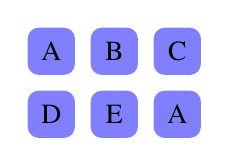
\begin{tikzpicture}[outer sep=0.05cm,node distance=0.8cm,]
\tikzstyle{bigbox} = [draw=white!50, thick, fill=white!10, rounded corners, rectangle]
\tikzstyle{box} = [minimum size=0.6cm, rounded corners,rectangle, fill=blue!50]
%
\node[box] (11) {A};
\node[box,right of=11] (12) {B};
\node[box,right of=12] (13) {C};
\node[box,below of=11] (21) {D};
\node[box,right of=21] (22) {E};
\node[box,right of=22] (23) {A};
\end{tikzpicture}
%\\
%The die is thrown once. What is the probability of getting (i) A? (ii) D?
}
%\resizebox{\columnwidth}{!}{

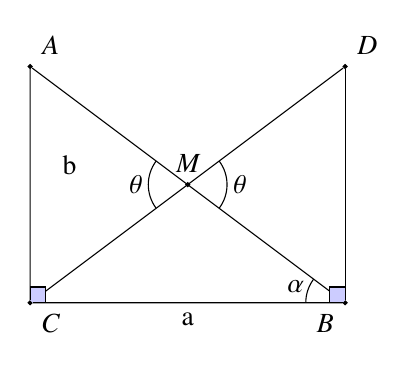
\begin{tikzpicture}
[scale=1,>=stealth,point/.style={draw,circle,fill = black,inner sep=0.5pt},]

%Triangle sides
\def\a{4}
\def\b{3}
\def\c{sqrt(\a^2+\c^2)}



%Labeling points
\node (A) at (0,\b)[point,label=above right:$A$] {};
\node (B) at (\a, 0)[point,label=below left:$B$] {};
\node (C) at (0, 0)[point,label=below right:$C$] {};
\node (M) at (\a*0.5,\b*0.5)[point,label=above:$M$] {};
\node (D) at (\a,\b)[point,label=above right:$D$] {};


%Drawing triangle ABC
\draw (A) -- node[left] {$\textrm{}$} (B) -- node[below] {$\textrm{a}$} (C) -- node[above,xshift=5mm] {$\textrm{b}$} (A);

%Joining CD
\draw (C)--(D);
%Joining BD
\draw (B)--(D);

%Drawing and marking angles
\tkzMarkAngle[fill=orange!40,size=0.5cm,mark=](A,M,C)
\tkzMarkAngle[fill=orange!40,size=0.5cm,mark=](B,M,D)
\tkzMarkAngle[fill=green!40,size=0.5cm,mark=](A,B,C)
\tkzMarkRightAngle[fill=blue!20,size=.2](A,C,B)
\tkzMarkRightAngle[fill=blue!20,size=.2](D,B,C)
\tkzLabelAngle[pos=0.65](A,M,C){$\theta$}
\tkzLabelAngle[pos=0.65](B,M,D){$\theta$}
\tkzLabelAngle[pos=0.65](A,B,C){$\alpha$}


\end{tikzpicture}
}
\caption{}
\label{fig:130_dice}	
\end{figure}

The die is thrown once. What is the probability of getting (i) A? (ii) D?
\\
\solution
Let X be the random variable representing the number of defective eggs from the ten eggs picked. X follows a  binomial distribution.  Since the probability of an egg being defective is 10\%, substituting n=10, p= 0.1 and k=0 in equation \eqref{eq:exam41_1}, 
probability that there is atleast one defective egg is 
\begin{align}
\pr{X \geq 1}&= 1 - \pr{X=0}  = 1-\brak{0.9}^{10}
\\
&=0.6513215599
\end{align}
The python code for the above problem is,
\begin{lstlisting}
.solutions/20-10/prob/codes/exam42.py
\end{lstlisting}

\item Which of the following arguments are correct and which are not correct? Give reasons
for your answer.\\
(i) If two coins are tossed simultaneously there are three possible outcomes—two
heads, two tails or one of each. Therefore, for each of these outcomes, the
probability is $\frac{1}{3}$ \\
(ii) If a die is thrown, there are two possible outcomes—an odd number or an even
number. Therefore, the probability of getting an odd number is $\frac{1}{2}$.
\\
\solution
\renewcommand{\theequation}{\theenumi}
\begin{enumerate}[label=\arabic*.,ref=\thesubsubsection.\theenumi]
\numberwithin{equation}{enumi}
\item In the given question,
\\
The sample size = Total number of possibilities(S)=6
\begin{align}
\myvec{1&2&3&4&5&6}
\end{align}
Event size= Odd number =3
\begin{align}
\myvec{1&3&5}
\end{align}
Probability for this event is = $\frac{1}{2}$
\\
The python code for the distribution of data,
\begin{lstlisting}
prob/codes/prob6_b.py
\end{lstlisting}
This shows the diagrametic representation of dice with the live update of probability with the role of dice.
\end{enumerate}

\item Two customers Shyam and Ekta are visiting a particular shop in the same week (Tuesday
to Saturday). Each is equally likely to visit the shop on any day as on another day. What
is the probability that both will visit the shop on\\
(i) the same day?\\
(ii) consecutive days?\\
(iii) different days?
\\
\solution
Let X be the random variable representing the number of defective eggs from the ten eggs picked. X follows a  binomial distribution.  Since the probability of an egg being defective is 10\%, substituting n=10, p= 0.1 and k=0 in equation \eqref{eq:exam41_1}, 
probability that there is atleast one defective egg is 
\begin{align}
\pr{X \geq 1}&= 1 - \pr{X=0}  = 1-\brak{0.9}^{10}
\\
&=0.6513215599
\end{align}
The python code for the above problem is,
\begin{lstlisting}
.solutions/20-10/prob/codes/exam42.py
\end{lstlisting}

\item A die is numbered in such a way that its faces show the numbers 1, 2, 2, 3, 3, 6. It is thrown two times and the total score in two throws is noted. Complete the following
table which gives a few values of the total score on the two throws:
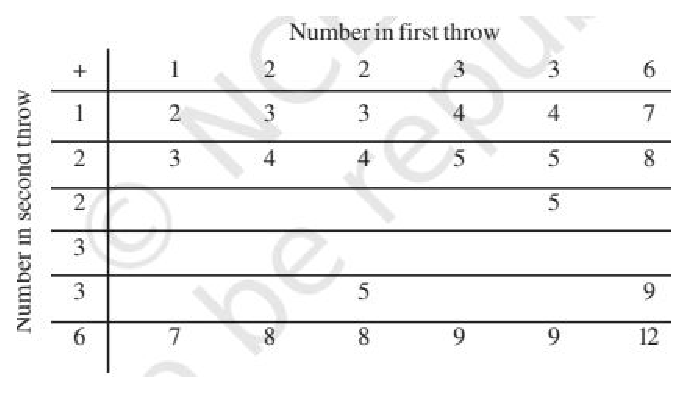
\includegraphics[width=\columnwidth]{./prob/figs/rows.eps}\\
What is the probability that the total score is
(i) even? (ii) 6? (iii) at least 6?
\\
\solution
Let X be the random variable representing the number of defective eggs from the ten eggs picked. X follows a  binomial distribution.  Since the probability of an egg being defective is 10\%, substituting n=10, p= 0.1 and k=0 in equation \eqref{eq:exam41_1}, 
probability that there is atleast one defective egg is 
\begin{align}
\pr{X \geq 1}&= 1 - \pr{X=0}  = 1-\brak{0.9}^{10}
\\
&=0.6513215599
\end{align}
The python code for the above problem is,
\begin{lstlisting}
.solutions/20-10/prob/codes/exam42.py
\end{lstlisting}


\end{enumerate}

 
\section{Axioms of Probability}

\renewcommand{\theequation}{\theenumi}
\begin{enumerate}[label=\thesection.\arabic*.,ref=\thesection.\theenumi]
\numberwithin{equation}{enumi}

\item Which of the following cannot be the probability of an event?\\
(A)$\frac{2}{3}$(B) –1.5 (C) 15 (D) 0.7
\\
\solution $0 < \pr{E} < 1$.  Hence, (B) and (C) are the right answer.
\item If P(E) = 0.05, what is the probability of ‘not E’?
%
\solution 
The desired probability is
\begin{align}
\pr{E^{\prime}} = 1 - \pr{E} = 0.95
\end{align}
%
\item If A and B are two events such that P(A) $\neq$ 0 and P(B/A) = 1, then
(A) A $\subset$ B \\
(B) B $\subset$ A \\
(C) B = $\phi$ \\
(D) A = $\phi$\\
\solution
Given 
\begin{align}
Pr(B | A)=1. 
\end{align}
By definition,
\begin{align}
Pr(B|A)=\frac{Pr(AB)}{Pr(A)}
\end{align}
\begin{align}
&\implies\frac{Pr(AB)}{Pr(A)} = 1\\
&\implies Pr(AB) = Pr(A)\label{1}\\
&\implies AB= A\label{2}
\end{align}
\begin{enumerate}[label={\Alph*)}]
\item Take any 
\begin{align}
    X \in A
\end{align} . From \eqref{2}, we get
\begin{align}
     X \in AB
\end{align}is also true.\\
Therefore, for any 
\begin{align}
  X \in A \\
  \implies X \in B   
\end{align}
    \begin{align}
     A \subseteq B 
\end{align}is also true.\\
    But, since A and B are two events,
    \begin{align}
       A\neq B 
    \end{align}. Hence,
    \begin{align}
    A \subset B
\end{align}
Therefore, option (A) is correct.
% \begin{figure}[h]
%     \centering
%     \includegraphics[width=8cm]{venn.png}
    
%     \label*{Venn diagram}
% \end{figure}
\item If 
\begin{align}
  B \subset A  
\end{align}
Then, 
\begin{align}
AB=B.
\end{align}
\begin{align}
\implies Pr(AB)=Pr(B)
\end{align}
But, from \eqref{1}, we have, 
\begin{align}
&Pr(AB)=Pr(A)\\
\implies &Pr(AB)=Pr(A)=Pr(B)
\end{align}
But,since A and B are two events, 
\begin{align}
    A\neq B
\end{align}. Hence, option (B) is incorrect.
 \item If 
 \begin{align}
     B=\phi
 \end{align}
\begin{align}
\implies Pr(AB)=0
\end{align}From \eqref{1}, we know that,
\begin{align}
& Pr(AB)=Pr(A)\\
\implies & Pr(AB)=Pr(A)=0
\end{align}
But,from the given data, we know that 
\begin{align}
     Pr(A) \neq 0
 \end{align}
Therefore,option C is incorrect.
\item If 
\begin{align}
     A=\phi
 \end{align}
\begin{align}
\implies Pr(A)=0
\end{align}
But,from the given data, we know that 
\begin{align}
     Pr(A) \neq 0
 \end{align}
Therefore,option D is incorrect.
\end{enumerate}

\item If P(A/B) $>$ P(A), then which of the following is correct :
(A) P(B/A) $<$ P(B) \\
(B) P(A $\cap$ B) $<$ P(A) . P(B)\\
(C) P(B/A) $>$ P(B) \\
(D) P(B/A) = P(B)
\solution
From the given information,
\begin{align}
    \label{eq:6.4.1}
    \frac{\pr{AB}}{\pr{B}}>\pr{A}\\
    \label{eq:6.4.2}
    \implies \pr{AB}>\pr{A}.\pr{B}
\end{align}
Hence, option (B) is false. Now, dividing the equation by \pr{A} on both sides i.e.,
\begin{align}
    \label{eq:6.4.3}
    \frac{\pr{AB}}{\pr{A}}>\pr{B}   
\end{align}
But $\frac{\pr{AB}}{\pr{A}}$ = \pr{B|A}. Therefore, from     \eqref{eq:6.4.3}
\begin{align}
    \label{eq:6.4.4}
    \pr{B|A}>\pr{B}
\end{align}
Hence, option (C) is correct.


\item If A and B are any two events such that P(A) + P(B) – P(A and B) = P(A), then\\
(A) P(B/A) = 1 \\
(B) P(A/B) = 1\\
(C) P(B/A) = 0 \\
(D) P(A/B) = 0\\
\item Complete the following statements:\\
 (i) Probability of an event E + Probability of the event ‘not E’ =----------- .\\
 (ii) The probability of an event that cannot happen is---------- . Such an event is called--------- .\\
 (iii) The probability of an event that is certain to happen is ---------.\\
 (iv) The sum of the probabilities of all the elementary events of an experiment is----------.\\ 
 (v) The probability of an event is greater than or equal to and less than or equal to --------------.\\
 %
 \solution
 \begin{enumerate}
 \item 1
 \item 0, null
 \item 1
 \item 1
 \item $0 \le \pr{E} \le 1$.
 \end{enumerate}
 \item An electronic assembly consists of two subsystems, say, A and B. From previous testing procedures, the following probabilities are assumed to be known:\\
P(A fails) = 0.2\\
P(B fails alone) = 0.15\\
P(A and B fail) = 0.15\\
\\Evaluate the following probabilities\\
(i) P(A fails|B has failed) \\
(ii) P(A fails alone)\\
\item A and B are two events such that P (A) $\neq$ 0. Find P(B/A), if\\
(i) A is a subset of B \\
(ii) A $\cap$ B = $\phi$\\
\solution
By definition,
%
\begin{align}
\pr{B|A} = \frac{\pr{AB}}{\pr{A}} 
\label{eq:axioms_6.8}
\end{align}
%
\begin{enumerate}
\item
\begin{align}
A &\subset B \implies \pr{AB} = \pr{A}
\\
\implies \pr{B|A} &= 1
\end{align}
%
upon substituting in \eqref{eq:axioms_6.8}
\item
\begin{align}
A \cup B = \phi \implies \pr{AB} = 0
\\
\implies \pr{B|A} &= 0
\end{align}
%
upon substituting in \eqref{eq:axioms_6.8}
\end{enumerate}
\item If A and B are two events such that A $\subset$ B and P(B) $\neq$ 0, then which of the following is correct?\\
\begin{enumerate}
\item P(A/B) = $\frac{P(B)}{P(A)}$
\item $P(A/B) < P(A)$
\item P(A/B) $\geq$ P(A)
\item None of these
\end{enumerate}
\item Let E and F be events with $\pr{E} = \frac{3}{5}$, $\pr{F} = \frac{3}{10}$ and  $\pr{E \cap F} = \frac{1}{5}$. Are E and F independent?
\\
\solution 
\begin{align}
\pr{E}\pr{F} = \frac{9}{50} \ne \pr{E \cap F}
\end{align}
%
Hence E and F are not independent.
\item Given that the events A and B are such that P(A) = $\frac{1}{2}$, P(A $\cup B$)= $\frac{3}{5}$ and P(B) = p. Find p if they are\\
(i) mutually exclusive\\
(ii) independent.\\

\item Let A and B be independent events with P(A) = 0.3 and P(B) = 0.4. Find\\
(i) P(A $\cap$ B)\\ 
(ii) P(A $\cup$ B)\\
(iii) P(A/B)\\
(iv) P(B/A)\\

\item If A and B are two events such that P(A) = $\frac{1}{4}$, P(B) = $\frac{1}{2}$ and P(A $\cap$ B) = $\frac{1}{8}$. find P (not A and not B).\\

\item Events A and B are such that P (A) = $\frac{1}{2}$, P(B) = $\frac{7}{12}$ and P(not A or not B) = $\frac{1}{4}$. State whether A and B are independent ?\\

\item Given two independent events A and B such that P(A) = 0.3, P(B) = 0.6. Find\\
(i) P(A and B)\\
(ii) P(A and not B)\\
(iii) P(A or B)\\
(iv) P(neither A nor B)\\
%
\solution
\begin{enumerate}[label={\roman*)}]
\item
Since the events A and B are independent events, by definition
\begin{align}
    \pr{A\, and\, B} = \pr{AB}= \pr{A}\pr{B}\label{6.15:a}
\end{align}
On substituting the values of \pr{A},\pr{B} in \eqref{6.15:a}, we get
\begin{align}
    \pr{A\, and\, B} &= \pr{A}\pr{B}\\
    &= (0.3)(0.6)\\
    \implies \pr{A\, and\, B}&=0.18
\end{align}
\item
As the events A and B are independent, then A and B' are also independent.
\begin{align}   
    \implies \pr{A\,and\,not\,B} &=\pr{AB'}\\
&= \pr{A}\pr{B'}\\
\therefore \pr{A\,and\,not\,B} &= \pr{A}\pr{B'}\label{6.15:b}
\end{align}
And we know that,
\begin{align}
    \pr{B'}=1-\pr{B}\label{6.15:c}
\end{align}
Using \eqref{6.15:c} in \eqref{6.15:b} we will get,
\begin{align}
   \pr{A\,and\,not\,B} &=\pr{AB'}\\
&= \pr{A}\pr{B'}\\
    \pr{A\,and\,not\,B} &= \pr{A}(1-\pr{B})\label{6.15:d}
\end{align}
On substituting the values of \pr{A},\pr{B} in \eqref{6.15:d}, we get
\begin{align}
    \pr{A\,and\,not\,B} &= 0.3(1-0.6)\\
    &= (0.3)(0.4)\\
    \implies \pr{A\,and\,not\,B}&= 0.12
\end{align}
\item
\begin{align}
    \pr{A\,or\,B} =\pr{A\,+\,B}\label{6.15:e}
\end{align}
We know that,
\begin{align}
    \pr{A\,+\,B} = \pr{A} + \pr{B} -\pr{AB}\label{6.15:f}
\end{align}
As events A and B are independent events,
\begin{align}
    \pr{AB}=\pr{A}\pr{B}\label{6.15:g}
\end{align}
Using \eqref{6.15:g} and \eqref{6.15:f} in \eqref{6.15:e}, We get
\begin{align}
    \pr{A\,+\,B} = \pr{A} + \pr{B} -\pr{A}\pr{B}\label{6.15:h}
\end{align}
On substituting the values of \pr{A},\pr{B} in \eqref{6.15:h}, we get
\begin{align}
    \pr{A\,or\,B} &= 0.3 + 0.6 -(0.3)(0.6)\\
    &= 0.9-0.18\\
    \implies \pr{A\,or\,B} &= 0.72\label{6.15:i}
\end{align}
\item
\begin{align}
    \pr{neither\, A\, nor\, B} &= \pr{A'B'}\\
    &=\pr{(A\,+\,B)'}\\
    \pr{neither\, A\, nor\, B}&=1-\pr{A\,+\,B}\label{6.15:j}
\end{align}
From \eqref{6.15:i},
\begin{align}
    \pr{A\,or\,B} =\pr{A\,+\,B}=0.72\label{6.15:k}
\end{align}
Using \eqref{6.15:k} in \eqref{6.15:j}, We get
\begin{align}
    \pr{neither\, A\, nor\, B}&=1-0.72\\
   \implies \pr{neither\, A\, nor\, B}&=0.28
\end{align}
\end{enumerate}
\item A die marked 1, 2, 3 in red and 4, 5, 6 in green is tossed. Let A be the event, 'the number is even,' and B be the event, 'the number is red'. Are A and B
independent?\\
\item A person plays a game of tossing a coin thrice. For each head, he is given Rs 2 by the organiser of the game and for each tail, he has to give Rs 1.50 to the organiser. Let X denote the amount gained or lost by the person. Show that X is a random variable and exhibit it as a function on the sample space of the experiment.\\

\item If $\pr{A}= \frac{7}{13}, \pr{B}=\frac{9}{13}$ and $\pr{AB}=\frac{4}{13},$ evaluate $\pr{A|B}$.
\\
\solution 
\begin{align}
\pr{A|B} = \frac{\pr{AB}}{\pr{B}} = \frac{4/13}{9/13} = \frac{4}{9}
\end{align}
\item A die is thrown. If E is the event "the number appearing is a multiple of 3" and F be the event "the number appearing is even" then find whether E and F are independent ?\\

\item An unbiased die is thrown twice. Let the event A be "odd number on the first throw" and B the event "odd number on the second throw". Check the independence of the events A and B.\\
\solution
\subsection{Problem}

\renewcommand{\theequation}{\theenumi}
\begin{enumerate}[label=\thesection.\arabic*.,ref=\thesection.\theenumi]
\numberwithin{equation}{enumi}
	\item  100 surnames were picked randomly from a telephone directory and the frequency distribution of the number of letters in english alphabet in surnames were obtained as follows.Determine the median number of letters in the surname and also find the modal size of the surnames. Also find the mean.\\
	
		\begin{table}[ht]
	\begin{center}
    	%%%%%%%%%%%%%%%%%%%%%%%%%%%%%%%%%%%%%%%%%%%%%%%%%%%%%%%%%%%%%%%%%%%%%%
%%                                                                  %%
%%  This is the header of a LaTeX2e file exported from Gnumeric.    %%
%%                                                                  %%
%%  This file can be compiled as it stands or included in another   %%
%%  LaTeX document. The table is based on the longtable package so  %%
%%  the longtable options (headers, footers...) can be set in the   %%
%%  preamble section below (see PRAMBLE).                           %%
%%                                                                  %%
%%  To include the file in another, the following two lines must be %%
%%  in the including file:                                          %%
%%        \def\inputGnumericTable{}                                 %%
%%  at the beginning of the file and:                               %%
%%        \input{name-of-this-file.tex}                             %%
%%  where the table is to be placed. Note also that the including   %%
%%  file must use the following packages for the table to be        %%
%%  rendered correctly:                                             %%
%%    \usepackage[latin1]{inputenc}                                 %%
%%    \usepackage{color}                                            %%
%%    \usepackage{array}                                            %%
%%    \usepackage{longtable}                                        %%
%%    \usepackage{calc}                                             %%
%%    \usepackage{multirow}                                         %%
%%    \usepackage{hhline}                                           %%
%%    \usepackage{ifthen}                                           %%
%%  optionally (for landscape tables embedded in another document): %%
%%    \usepackage{lscape}                                           %%
%%                                                                  %%
%%%%%%%%%%%%%%%%%%%%%%%%%%%%%%%%%%%%%%%%%%%%%%%%%%%%%%%%%%%%%%%%%%%%%%



%%  This section checks if we are begin input into another file or  %%
%%  the file will be compiled alone. First use a macro taken from   %%
%%  the TeXbook ex 7.7 (suggestion of Han-Wen Nienhuys).            %%
\def\ifundefined#1{\expandafter\ifx\csname#1\endcsname\relax}


%%  Check for the \def token for inputed files. If it is not        %%
%%  defined, the file will be processed as a standalone and the     %%
%%  preamble will be used.                                          %%
\ifundefined{inputGnumericTable}

%%  We must be able to close or not the document at the end.        %%
	\def\gnumericTableEnd{\end{document}}


%%%%%%%%%%%%%%%%%%%%%%%%%%%%%%%%%%%%%%%%%%%%%%%%%%%%%%%%%%%%%%%%%%%%%%
%%                                                                  %%
%%  This is the PREAMBLE. Change these values to get the right      %%
%%  paper size and other niceties.                                  %%
%%                                                                  %%
%%%%%%%%%%%%%%%%%%%%%%%%%%%%%%%%%%%%%%%%%%%%%%%%%%%%%%%%%%%%%%%%%%%%%%

	\documentclass[12pt%
			  %,landscape%
                    ]{report}
       \usepackage[latin1]{inputenc}
       \usepackage{fullpage}
       \usepackage{color}
       \usepackage{array}
       \usepackage{longtable}
       \usepackage{calc}
       \usepackage{multirow}
       \usepackage{hhline}
       \usepackage{ifthen}

	\begin{document}


%%  End of the preamble for the standalone. The next section is for %%
%%  documents which are included into other LaTeX2e files.          %%
\else

%%  We are not a stand alone document. For a regular table, we will %%
%%  have no preamble and only define the closing to mean nothing.   %%
    \def\gnumericTableEnd{}

%%  If we want landscape mode in an embedded document, comment out  %%
%%  the line above and uncomment the two below. The table will      %%
%%  begin on a new page and run in landscape mode.                  %%
%       \def\gnumericTableEnd{\end{landscape}}
%       \begin{landscape}


%%  End of the else clause for this file being \input.              %%
\fi

%%%%%%%%%%%%%%%%%%%%%%%%%%%%%%%%%%%%%%%%%%%%%%%%%%%%%%%%%%%%%%%%%%%%%%
%%                                                                  %%
%%  The rest is the gnumeric table, except for the closing          %%
%%  statement. Changes below will alter the table's appearance.     %%
%%                                                                  %%
%%%%%%%%%%%%%%%%%%%%%%%%%%%%%%%%%%%%%%%%%%%%%%%%%%%%%%%%%%%%%%%%%%%%%%

\providecommand{\gnumericmathit}[1]{#1} 
%%  Uncomment the next line if you would like your numbers to be in %%
%%  italics if they are italizised in the gnumeric table.           %%
%\renewcommand{\gnumericmathit}[1]{\mathit{#1}}
\providecommand{\gnumericPB}[1]%
{\let\gnumericTemp=\\#1\let\\=\gnumericTemp\hspace{0pt}}
 \ifundefined{gnumericTableWidthDefined}
        \newlength{\gnumericTableWidth}
        \newlength{\gnumericTableWidthComplete}
        \newlength{\gnumericMultiRowLength}
        \global\def\gnumericTableWidthDefined{}
 \fi
%% The following setting protects this code from babel shorthands.  %%
 \ifthenelse{\isundefined{\languageshorthands}}{}{\languageshorthands{english}}
%%  The default table format retains the relative column widths of  %%
%%  gnumeric. They can easily be changed to c, r or l. In that case %%
%%  you may want to comment out the next line and uncomment the one %%
%%  thereafter                                                      %%
\providecommand\gnumbox{\makebox[0pt]}
%%\providecommand\gnumbox[1][]{\makebox}

%% to adjust positions in multirow situations                       %%
\setlength{\bigstrutjot}{\jot}
\setlength{\extrarowheight}{\doublerulesep}

%%  The \setlongtables command keeps column widths the same across  %%
%%  pages. Simply comment out next line for varying column widths.  %%
\setlongtables

\setlength\gnumericTableWidth{%
	53pt+%
	53pt+%
	53pt+%
0pt}
\def\gumericNumCols{3}
\setlength\gnumericTableWidthComplete{\gnumericTableWidth+%
         \tabcolsep*\gumericNumCols*2+\arrayrulewidth*\gumericNumCols}
\ifthenelse{\lengthtest{\gnumericTableWidthComplete > \linewidth}}%
         {\def\gnumericScale{\ratio{\linewidth-%
                        \tabcolsep*\gumericNumCols*2-%
                        \arrayrulewidth*\gumericNumCols}%
{\gnumericTableWidth}}}%
{\def\gnumericScale{1}}

%%%%%%%%%%%%%%%%%%%%%%%%%%%%%%%%%%%%%%%%%%%%%%%%%%%%%%%%%%%%%%%%%%%%%%
%%                                                                  %%
%% The following are the widths of the various columns. We are      %%
%% defining them here because then they are easier to change.       %%
%% Depending on the cell formats we may use them more than once.    %%
%%                                                                  %%
%%%%%%%%%%%%%%%%%%%%%%%%%%%%%%%%%%%%%%%%%%%%%%%%%%%%%%%%%%%%%%%%%%%%%%

\ifthenelse{\isundefined{\gnumericColA}}{\newlength{\gnumericColA}}{}\settowidth{\gnumericColA}{\begin{tabular}{@{}p{53pt*\gnumericScale}@{}}x\end{tabular}}
\ifthenelse{\isundefined{\gnumericColB}}{\newlength{\gnumericColB}}{}\settowidth{\gnumericColB}{\begin{tabular}{@{}p{53pt*\gnumericScale}@{}}x\end{tabular}}
\ifthenelse{\isundefined{\gnumericColC}}{\newlength{\gnumericColC}}{}\settowidth{\gnumericColC}{\begin{tabular}{@{}p{53pt*\gnumericScale}@{}}x\end{tabular}}

\begin{tabular}[c]{%
	b{\gnumericColA}%
	b{\gnumericColB}%
	b{\gnumericColC}%
	}

%%%%%%%%%%%%%%%%%%%%%%%%%%%%%%%%%%%%%%%%%%%%%%%%%%%%%%%%%%%%%%%%%%%%%%
%%  The longtable options. (Caption, headers... see Goosens, p.124) %%
%	\caption{The Table Caption.}             \\	%
% \hline	% Across the top of the table.
%%  The rest of these options are table rows which are placed on    %%
%%  the first, last or every page. Use \multicolumn if you want.    %%

%%  Header for the first page.                                      %%
%	\multicolumn{3}{c}{The First Header} \\ \hline 
%	\multicolumn{1}{c}{colTag}	%Column 1
%	&\multicolumn{1}{c}{colTag}	%Column 2
%	&\multicolumn{1}{c}{colTag}	\\ \hline %Last column
%	\endfirsthead

%%  The running header definition.                                  %%
%	\hline
%	\multicolumn{3}{l}{\ldots\small\slshape continued} \\ \hline
%	\multicolumn{1}{c}{colTag}	%Column 1
%	&\multicolumn{1}{c}{colTag}	%Column 2
%	&\multicolumn{1}{c}{colTag}	\\ \hline %Last column
%	\endhead

%%  The running footer definition.                                  %%
%	\hline
%	\multicolumn{3}{r}{\small\slshape continued\ldots} \\
%	\endfoot

%%  The ending footer definition.                                   %%
%	\multicolumn{3}{c}{That's all folks} \\ \hline 
%	\endlastfoot
%%%%%%%%%%%%%%%%%%%%%%%%%%%%%%%%%%%%%%%%%%%%%%%%%%%%%%%%%%%%%%%%%%%%%%

\hhline{|-|-|-}
	 \multicolumn{1}{|p{\gnumericColA}|}%
	{\gnumericPB{\raggedright}\gnumbox[l]{No.of.letters}}
	&\multicolumn{1}{p{\gnumericColB}|}%
	{\gnumericPB{\raggedright}\gnumbox[l]{Surnames}}
	&\multicolumn{1}{p{\gnumericColC}|}%
	{\gnumericPB{\raggedright}\gnumbox[l]{Cum.Freq}}
\\
\hhline{|---|}
	 \multicolumn{1}{|p{\gnumericColA}|}%
	{\gnumericPB{\raggedright}\gnumbox[l]{001-004}}
	&\multicolumn{1}{p{\gnumericColB}|}%
	{\gnumericPB{\raggedright}\gnumbox[l]{6}}
	&\multicolumn{1}{p{\gnumericColC}|}%
	{\gnumericPB{\raggedright}\gnumbox[l]{6}}
\\
\hhline{|---|}
	 \multicolumn{1}{|p{\gnumericColA}|}%
	{\gnumericPB{\raggedright}\gnumbox[l]{004-007}}
	&\multicolumn{1}{p{\gnumericColB}|}%
	{\gnumericPB{\raggedright}\gnumbox[l]{30}}
	&\multicolumn{1}{p{\gnumericColC}|}%
	{\gnumericPB{\raggedright}\gnumbox[l]{36}}
\\
\hhline{|---|}
	 \multicolumn{1}{|p{\gnumericColA}|}%
	{\gnumericPB{\raggedright}\gnumbox[l]{007-010}}
	&\multicolumn{1}{p{\gnumericColB}|}%
	{\gnumericPB{\raggedright}\gnumbox[l]{40}}
	&\multicolumn{1}{p{\gnumericColC}|}%
	{\gnumericPB{\raggedright}\gnumbox[l]{76}}
\\
\hhline{|---|}
	 \multicolumn{1}{|p{\gnumericColA}|}%
	{\gnumericPB{\raggedright}\gnumbox[l]{10-13}}
	&\multicolumn{1}{p{\gnumericColB}|}%
	{\gnumericPB{\raggedright}\gnumbox[l]{16}}
	&\multicolumn{1}{p{\gnumericColC}|}%
	{\gnumericPB{\raggedright}\gnumbox[l]{92}}
\\
\hhline{|---|}
	 \multicolumn{1}{|p{\gnumericColA}|}%
	{\gnumericPB{\raggedright}\gnumbox[l]{13-16}}
	&\multicolumn{1}{p{\gnumericColB}|}%
	{\gnumericPB{\raggedright}\gnumbox[l]{4}}
	&\multicolumn{1}{p{\gnumericColC}|}%
	{\gnumericPB{\raggedright}\gnumbox[l]{96}}
\\
\hhline{|---|}
	 \multicolumn{1}{|p{\gnumericColA}|}%
	{\gnumericPB{\raggedright}\gnumbox[l]{16-19}}
	&\multicolumn{1}{p{\gnumericColB}|}%
	{\gnumericPB{\raggedright}\gnumbox[l]{4}}
	&\multicolumn{1}{p{\gnumericColC}|}%
	{\gnumericPB{\raggedright}\gnumbox[l]{100}}
\\
\hhline{|-|-|-|}
\end{tabular}

\ifthenelse{\isundefined{\languageshorthands}}{}{\languageshorthands{\languagename}}
\gnumericTableEnd

	\caption{Frequency distribution of the number of letters in surname}
	\label{table:table10}
	\end{center}
	\end{table}
	
	
	
	\solution  The following python code computes the mean, median and mode.
	\begin{lstlisting}
	codes/statistics/exercises/q21.py
	\end{lstlisting}
	
	\begin{align}
	\text{Median} &= l + \frac{\frac{n}{2} -cf}{f}\times h
	\end{align}
	\begin{align}
	\text{n} = \sum f_{i} = 100 \implies \frac{n}{2} = 50\\
	\end{align}
	$\therefore$ 7-10 is the median class.\\
	Here l is the lower limit of the median class = 7\\
	h is the classinterval =3\\
	cf is the cumulative frequency of the class before median class = 36\\
	f is the frequency of the median class



	\begin{table}[ht]
	\begin{center}
    	%%%%%%%%%%%%%%%%%%%%%%%%%%%%%%%%%%%%%%%%%%%%%%%%%%%%%%%%%%%%%%%%%%%%%%
%%                                                                  %%
%%  This is the header of a LaTeX2e file exported from Gnumeric.    %%
%%                                                                  %%
%%  This file can be compiled as it stands or included in another   %%
%%  LaTeX document. The table is based on the longtable package so  %%
%%  the longtable options (headers, footers...) can be set in the   %%
%%  preamble section below (see PRAMBLE).                           %%
%%                                                                  %%
%%  To include the file in another, the following two lines must be %%
%%  in the including file:                                          %%
%%        \def\inputGnumericTable{}                                 %%
%%  at the beginning of the file and:                               %%
%%        \input{name-of-this-file.tex}                             %%
%%  where the table is to be placed. Note also that the including   %%
%%  file must use the following packages for the table to be        %%
%%  rendered correctly:                                             %%
%%    \usepackage[latin1]{inputenc}                                 %%
%%    \usepackage{color}                                            %%
%%    \usepackage{array}                                            %%
%%    \usepackage{longtable}                                        %%
%%    \usepackage{calc}                                             %%
%%    \usepackage{multirow}                                         %%
%%    \usepackage{hhline}                                           %%
%%    \usepackage{ifthen}                                           %%
%%  optionally (for landscape tables embedded in another document): %%
%%    \usepackage{lscape}                                           %%
%%                                                                  %%
%%%%%%%%%%%%%%%%%%%%%%%%%%%%%%%%%%%%%%%%%%%%%%%%%%%%%%%%%%%%%%%%%%%%%%



%%  This section checks if we are begin input into another file or  %%
%%  the file will be compiled alone. First use a macro taken from   %%
%%  the TeXbook ex 7.7 (suggestion of Han-Wen Nienhuys).            %%
\def\ifundefined#1{\expandafter\ifx\csname#1\endcsname\relax}


%%  Check for the \def token for inputed files. If it is not        %%
%%  defined, the file will be processed as a standalone and the     %%
%%  preamble will be used.                                          %%
\ifundefined{inputGnumericTable}

%%  We must be able to close or not the document at the end.        %%
	\def\gnumericTableEnd{\end{document}}


%%%%%%%%%%%%%%%%%%%%%%%%%%%%%%%%%%%%%%%%%%%%%%%%%%%%%%%%%%%%%%%%%%%%%%
%%                                                                  %%
%%  This is the PREAMBLE. Change these values to get the right      %%
%%  paper size and other niceties.                                  %%
%%                                                                  %%
%%%%%%%%%%%%%%%%%%%%%%%%%%%%%%%%%%%%%%%%%%%%%%%%%%%%%%%%%%%%%%%%%%%%%%

	\documentclass[12pt%
			  %,landscape%
                    ]{report}
       \usepackage[latin1]{inputenc}
       \usepackage{fullpage}
       \usepackage{color}
       \usepackage{array}
       \usepackage{longtable}
       \usepackage{calc}
       \usepackage{multirow}
       \usepackage{hhline}
       \usepackage{ifthen}

	\begin{document}


%%  End of the preamble for the standalone. The next section is for %%
%%  documents which are included into other LaTeX2e files.          %%
\else

%%  We are not a stand alone document. For a regular table, we will %%
%%  have no preamble and only define the closing to mean nothing.   %%
    \def\gnumericTableEnd{}

%%  If we want landscape mode in an embedded document, comment out  %%
%%  the line above and uncomment the two below. The table will      %%
%%  begin on a new page and run in landscape mode.                  %%
%       \def\gnumericTableEnd{\end{landscape}}
%       \begin{landscape}


%%  End of the else clause for this file being \input.              %%
\fi

%%%%%%%%%%%%%%%%%%%%%%%%%%%%%%%%%%%%%%%%%%%%%%%%%%%%%%%%%%%%%%%%%%%%%%
%%                                                                  %%
%%  The rest is the gnumeric table, except for the closing          %%
%%  statement. Changes below will alter the table's appearance.     %%
%%                                                                  %%
%%%%%%%%%%%%%%%%%%%%%%%%%%%%%%%%%%%%%%%%%%%%%%%%%%%%%%%%%%%%%%%%%%%%%%

\providecommand{\gnumericmathit}[1]{#1} 
%%  Uncomment the next line if you would like your numbers to be in %%
%%  italics if they are italizised in the gnumeric table.           %%
%\renewcommand{\gnumericmathit}[1]{\mathit{#1}}
\providecommand{\gnumericPB}[1]%
{\let\gnumericTemp=\\#1\let\\=\gnumericTemp\hspace{0pt}}
 \ifundefined{gnumericTableWidthDefined}
        \newlength{\gnumericTableWidth}
        \newlength{\gnumericTableWidthComplete}
        \newlength{\gnumericMultiRowLength}
        \global\def\gnumericTableWidthDefined{}
 \fi
%% The following setting protects this code from babel shorthands.  %%
 \ifthenelse{\isundefined{\languageshorthands}}{}{\languageshorthands{english}}
%%  The default table format retains the relative column widths of  %%
%%  gnumeric. They can easily be changed to c, r or l. In that case %%
%%  you may want to comment out the next line and uncomment the one %%
%%  thereafter                                                      %%
\providecommand\gnumbox{\makebox[0pt]}
%%\providecommand\gnumbox[1][]{\makebox}

%% to adjust positions in multirow situations                       %%
\setlength{\bigstrutjot}{\jot}
\setlength{\extrarowheight}{\doublerulesep}

%%  The \setlongtables command keeps column widths the same across  %%
%%  pages. Simply comment out next line for varying column widths.  %%
\setlongtables

\setlength\gnumericTableWidth{%
	53pt+%
	25pt+%
	43pt+%
	29pt+%
0pt}
\def\gumericNumCols{4}
\setlength\gnumericTableWidthComplete{\gnumericTableWidth+%
         \tabcolsep*\gumericNumCols*2+\arrayrulewidth*\gumericNumCols}
\ifthenelse{\lengthtest{\gnumericTableWidthComplete > \linewidth}}%
         {\def\gnumericScale{\ratio{\linewidth-%
                        \tabcolsep*\gumericNumCols*2-%
                        \arrayrulewidth*\gumericNumCols}%
{\gnumericTableWidth}}}%
{\def\gnumericScale{1}}

%%%%%%%%%%%%%%%%%%%%%%%%%%%%%%%%%%%%%%%%%%%%%%%%%%%%%%%%%%%%%%%%%%%%%%
%%                                                                  %%
%% The following are the widths of the various columns. We are      %%
%% defining them here because then they are easier to change.       %%
%% Depending on the cell formats we may use them more than once.    %%
%%                                                                  %%
%%%%%%%%%%%%%%%%%%%%%%%%%%%%%%%%%%%%%%%%%%%%%%%%%%%%%%%%%%%%%%%%%%%%%%

\ifthenelse{\isundefined{\gnumericColA}}{\newlength{\gnumericColA}}{}\settowidth{\gnumericColA}{\begin{tabular}{@{}p{53pt*\gnumericScale}@{}}x\end{tabular}}
\ifthenelse{\isundefined{\gnumericColB}}{\newlength{\gnumericColB}}{}\settowidth{\gnumericColB}{\begin{tabular}{@{}p{25pt*\gnumericScale}@{}}x\end{tabular}}
\ifthenelse{\isundefined{\gnumericColC}}{\newlength{\gnumericColC}}{}\settowidth{\gnumericColC}{\begin{tabular}{@{}p{43pt*\gnumericScale}@{}}x\end{tabular}}
\ifthenelse{\isundefined{\gnumericColD}}{\newlength{\gnumericColD}}{}\settowidth{\gnumericColD}{\begin{tabular}{@{}p{29pt*\gnumericScale}@{}}x\end{tabular}}

\begin{tabular}[c]{%
	b{\gnumericColA}%
	b{\gnumericColB}%
	b{\gnumericColC}%
	b{\gnumericColD}%
	}

%%%%%%%%%%%%%%%%%%%%%%%%%%%%%%%%%%%%%%%%%%%%%%%%%%%%%%%%%%%%%%%%%%%%%%
%%  The longtable options. (Caption, headers... see Goosens, p.124) %%
%	\caption{The Table Caption.}             \\	%
% \hline	% Across the top of the table.
%%  The rest of these options are table rows which are placed on    %%
%%  the first, last or every page. Use \multicolumn if you want.    %%

%%  Header for the first page.                                      %%
%	\multicolumn{4}{c}{The First Header} \\ \hline 
%	\multicolumn{1}{c}{colTag}	%Column 1
%	&\multicolumn{1}{c}{colTag}	%Column 2
%	&\multicolumn{1}{c}{colTag}	%Column 3
%	&\multicolumn{1}{c}{colTag}	\\ \hline %Last column
%	\endfirsthead

%%  The running header definition.                                  %%
%	\hline
%	\multicolumn{4}{l}{\ldots\small\slshape continued} \\ \hline
%	\multicolumn{1}{c}{colTag}	%Column 1
%	&\multicolumn{1}{c}{colTag}	%Column 2
%	&\multicolumn{1}{c}{colTag}	%Column 3
%	&\multicolumn{1}{c}{colTag}	\\ \hline %Last column
%	\endhead

%%  The running footer definition.                                  %%
%	\hline
%	\multicolumn{4}{r}{\small\slshape continued\ldots} \\
%	\endfoot

%%  The ending footer definition.                                   %%
%	\multicolumn{4}{c}{That's all folks} \\ \hline 
%	\endlastfoot
%%%%%%%%%%%%%%%%%%%%%%%%%%%%%%%%%%%%%%%%%%%%%%%%%%%%%%%%%%%%%%%%%%%%%%

\hhline{|-|-|-|-}
	 \multicolumn{1}{|p{\gnumericColA}|}%
	{\gnumericPB{\raggedright}\gnumbox[l]{No.of.letters}}
	&\multicolumn{1}{p{\gnumericColB}|}%
	{\gnumericPB{\raggedright}\gnumbox[l]{$f_i$}}
	&\multicolumn{1}{p{\gnumericColC}|}%
	{\gnumericPB{\raggedright}\gnumbox[l]{$x_i$}}
	&\multicolumn{1}{p{\gnumericColD}|}%
	{\gnumericPB{\raggedright}\gnumbox[l]{$f_ix_i$}}
\\
\hhline{|----|}
	 \multicolumn{1}{|p{\gnumericColA}|}%
	{\gnumericPB{\raggedright}\gnumbox[l]{001-004}}
	&\multicolumn{1}{p{\gnumericColB}|}%
	{\gnumericPB{\raggedright}\gnumbox[l]{6}}
	&\multicolumn{1}{p{\gnumericColC}|}%
	{\gnumericPB{\raggedright}\gnumbox[l]{2.5}}
	&\multicolumn{1}{p{\gnumericColD}|}%
	{\gnumericPB{\raggedright}\gnumbox[l]{15}}
\\
\hhline{|----|}
	 \multicolumn{1}{|p{\gnumericColA}|}%
	{\gnumericPB{\raggedright}\gnumbox[l]{004-007}}
	&\multicolumn{1}{p{\gnumericColB}|}%
	{\gnumericPB{\raggedright}\gnumbox[l]{30}}
	&\multicolumn{1}{p{\gnumericColC}|}%
	{\gnumericPB{\raggedright}\gnumbox[l]{5.5}}
	&\multicolumn{1}{p{\gnumericColD}|}%
	{\gnumericPB{\raggedright}\gnumbox[l]{165}}
\\
\hhline{|----|}
	 \multicolumn{1}{|p{\gnumericColA}|}%
	{\gnumericPB{\raggedright}\gnumbox[l]{007-010}}
	&\multicolumn{1}{p{\gnumericColB}|}%
	{\gnumericPB{\raggedright}\gnumbox[l]{40}}
	&\multicolumn{1}{p{\gnumericColC}|}%
	{\gnumericPB{\raggedright}\gnumbox[l]{8.5}}
	&\multicolumn{1}{p{\gnumericColD}|}%
	{\gnumericPB{\raggedright}\gnumbox[l]{340}}
\\
\hhline{|----|}
	 \multicolumn{1}{|p{\gnumericColA}|}%
	{\gnumericPB{\raggedright}\gnumbox[l]{10-13}}
	&\multicolumn{1}{p{\gnumericColB}|}%
	{\gnumericPB{\raggedright}\gnumbox[l]{16}}
	&\multicolumn{1}{p{\gnumericColC}|}%
	{\gnumericPB{\raggedright}\gnumbox[l]{11.5}}
	&\multicolumn{1}{p{\gnumericColD}|}%
	{\gnumericPB{\raggedright}\gnumbox[l]{184}}
\\
\hhline{|----|}
	 \multicolumn{1}{|p{\gnumericColA}|}%
	{\gnumericPB{\raggedright}\gnumbox[l]{13-16}}
	&\multicolumn{1}{p{\gnumericColB}|}%
	{\gnumericPB{\raggedright}\gnumbox[l]{4}}
	&\multicolumn{1}{p{\gnumericColC}|}%
	{\gnumericPB{\raggedright}\gnumbox[l]{14.5}}
	&\multicolumn{1}{p{\gnumericColD}|}%
	{\gnumericPB{\raggedright}\gnumbox[l]{58}}
\\
\hhline{|----|}
	 \multicolumn{1}{|p{\gnumericColA}|}%
	{\gnumericPB{\raggedright}\gnumbox[l]{16-19}}
	&\multicolumn{1}{p{\gnumericColB}|}%
	{\gnumericPB{\raggedright}\gnumbox[l]{4}}
	&\multicolumn{1}{p{\gnumericColC}|}%
	{\gnumericPB{\raggedright}\gnumbox[l]{17.5}}
	&\multicolumn{1}{p{\gnumericColD}|}%
	{\gnumericPB{\raggedright}\gnumbox[l]{70}}
\\
\hhline{|-|-|-|-|}
\end{tabular}

\ifthenelse{\isundefined{\languageshorthands}}{}{\languageshorthands{\languagename}}
\gnumericTableEnd

	\caption{Frequency distribution of the number of letters in surname}
	\label{table:table10}
	\end{center}
	\end{table}
	\begin{align}
	\text{Mean} &= \frac{\sum f_ix_i}{\sum f_i}\\
	\text{Mean} &= \frac{832}{100}\\
	\text{Mean} &= 8.32
	\end{align}

	\begin{align}
	\text{Median} &= 7 + \frac{50 - 36}{40}\times 3\\
	\text{Median} &= 7 + 1.05 = 8.05
	\end{align}
	Hence median no. of letters is 8.05
	\begin{align}
	\text{Mode} &= l + \frac{f_1 - f_0}{2f_1 - f_0 - f_2} \times h
	\end{align}
	Modal class is the interval with the highest frequency = 7-10, where\\
	l is lower limit of the modal class = 7\\
	h is the class interval = 4-1=3\\
	$f_1$ is the frequency of the modal class = 40\\
	$f_0$ is frequency of the class before modal class = 30\\
	$f_2$ is frequency of the class after modal class = 16\\
	\begin{align}
	\text{Mode} &= 7 + \frac{40-30}{80-30-16} \times 3
	\end{align}	
	which is calculated as 7.88
	
\end{enumerate}



\item Prove that if E and F are independent events, then so are the events E and $F^{'}$.\\
\solution

	\begin{table}[ht]
    \begin{center}
    	%%%%%%%%%%%%%%%%%%%%%%%%%%%%%%%%%%%%%%%%%%%%%%%%%%%%%%%%%%%%%%%%%%%%%%
%%                                                                  %%
%%  This is the header of a LaTeX2e file exported from Gnumeric.    %%
%%                                                                  %%
%%  This file can be compiled as it stands or included in another   %%
%%  LaTeX document. The table is based on the longtable package so  %%
%%  the longtable options (headers, footers...) can be set in the   %%
%%  preamble section below (see PRAMBLE).                           %%
%%                                                                  %%
%%  To include the file in another, the following two lines must be %%
%%  in the including file:                                          %%
%%        \def\inputGnumericTable{}                                 %%
%%  at the beginning of the file and:                               %%
%%        \input{name-of-this-file.tex}                             %%
%%  where the table is to be placed. Note also that the including   %%
%%  file must use the following packages for the table to be        %%
%%  rendered correctly:                                             %%
%%    \usepackage[latin1]{inputenc}                                 %%
%%    \usepackage{color}                                            %%
%%    \usepackage{array}                                            %%
%%    \usepackage{longtable}                                        %%
%%    \usepackage{calc}                                             %%
%%    \usepackage{multirow}                                         %%
%%    \usepackage{hhline}                                           %%
%%    \usepackage{ifthen}                                           %%
%%  optionally (for landscape tables embedded in another document): %%
%%    \usepackage{lscape}                                           %%
%%                                                                  %%
%%%%%%%%%%%%%%%%%%%%%%%%%%%%%%%%%%%%%%%%%%%%%%%%%%%%%%%%%%%%%%%%%%%%%%



%%  This section checks if we are begin input into another file or  %%
%%  the file will be compiled alone. First use a macro taken from   %%
%%  the TeXbook ex 7.7 (suggestion of Han-Wen Nienhuys).            %%
\def\ifundefined#1{\expandafter\ifx\csname#1\endcsname\relax}


%%  Check for the \def token for inputed files. If it is not        %%
%%  defined, the file will be processed as a standalone and the     %%
%%  preamble will be used.                                          %%
\ifundefined{inputGnumericTable}

%%  We must be able to close or not the document at the end.        %%
	\def\gnumericTableEnd{\end{document}}


%%%%%%%%%%%%%%%%%%%%%%%%%%%%%%%%%%%%%%%%%%%%%%%%%%%%%%%%%%%%%%%%%%%%%%
%%                                                                  %%
%%  This is the PREAMBLE. Change these values to get the right      %%
%%  paper size and other niceties.                                  %%
%%                                                                  %%
%%%%%%%%%%%%%%%%%%%%%%%%%%%%%%%%%%%%%%%%%%%%%%%%%%%%%%%%%%%%%%%%%%%%%%

	\documentclass[12pt%
			  %,landscape%
                    ]{report}
       \usepackage[latin1]{inputenc}
       \usepackage{fullpage}
       \usepackage{color}
       \usepackage{array}
       \usepackage{longtable}
       \usepackage{calc}
       \usepackage{multirow}
       \usepackage{hhline}
       \usepackage{ifthen}

	\begin{document}


%%  End of the preamble for the standalone. The next section is for %%
%%  documents which are included into other LaTeX2e files.          %%
\else

%%  We are not a stand alone document. For a regular table, we will %%
%%  have no preamble and only define the closing to mean nothing.   %%
    \def\gnumericTableEnd{}

%%  If we want landscape mode in an embedded document, comment out  %%
%%  the line above and uncomment the two below. The table will      %%
%%  begin on a new page and run in landscape mode.                  %%
%       \def\gnumericTableEnd{\end{landscape}}
%       \begin{landscape}


%%  End of the else clause for this file being \input.              %%
\fi

%%%%%%%%%%%%%%%%%%%%%%%%%%%%%%%%%%%%%%%%%%%%%%%%%%%%%%%%%%%%%%%%%%%%%%
%%                                                                  %%
%%  The rest is the gnumeric table, except for the closing          %%
%%  statement. Changes below will alter the table's appearance.     %%
%%                                                                  %%
%%%%%%%%%%%%%%%%%%%%%%%%%%%%%%%%%%%%%%%%%%%%%%%%%%%%%%%%%%%%%%%%%%%%%%

\providecommand{\gnumericmathit}[1]{#1} 
%%  Uncomment the next line if you would like your numbers to be in %%
%%  italics if they are italizised in the gnumeric table.           %%
%\renewcommand{\gnumericmathit}[1]{\mathit{#1}}
\providecommand{\gnumericPB}[1]%
{\let\gnumericTemp=\\#1\let\\=\gnumericTemp\hspace{0pt}}
 \ifundefined{gnumericTableWidthDefined}
        \newlength{\gnumericTableWidth}
        \newlength{\gnumericTableWidthComplete}
        \newlength{\gnumericMultiRowLength}
        \global\def\gnumericTableWidthDefined{}
 \fi
%% The following setting protects this code from babel shorthands.  %%
 \ifthenelse{\isundefined{\languageshorthands}}{}{\languageshorthands{english}}
%%  The default table format retains the relative column widths of  %%
%%  gnumeric. They can easily be changed to c, r or l. In that case %%
%%  you may want to comment out the next line and uncomment the one %%
%%  thereafter                                                      %%
\providecommand\gnumbox{\makebox[0pt]}
%%\providecommand\gnumbox[1][]{\makebox}

%% to adjust positions in multirow situations                       %%
\setlength{\bigstrutjot}{\jot}
\setlength{\extrarowheight}{\doublerulesep}

%%  The \setlongtables command keeps column widths the same across  %%
%%  pages. Simply comment out next line for varying column widths.  %%
\setlongtables

\setlength\gnumericTableWidth{%
	53pt+%
	53pt+%
	53pt+%
0pt}
\def\gumericNumCols{3}
\setlength\gnumericTableWidthComplete{\gnumericTableWidth+%
         \tabcolsep*\gumericNumCols*2+\arrayrulewidth*\gumericNumCols}
\ifthenelse{\lengthtest{\gnumericTableWidthComplete > \linewidth}}%
         {\def\gnumericScale{\ratio{\linewidth-%
                        \tabcolsep*\gumericNumCols*2-%
                        \arrayrulewidth*\gumericNumCols}%
{\gnumericTableWidth}}}%
{\def\gnumericScale{1}}

%%%%%%%%%%%%%%%%%%%%%%%%%%%%%%%%%%%%%%%%%%%%%%%%%%%%%%%%%%%%%%%%%%%%%%
%%                                                                  %%
%% The following are the widths of the various columns. We are      %%
%% defining them here because then they are easier to change.       %%
%% Depending on the cell formats we may use them more than once.    %%
%%                                                                  %%
%%%%%%%%%%%%%%%%%%%%%%%%%%%%%%%%%%%%%%%%%%%%%%%%%%%%%%%%%%%%%%%%%%%%%%

\ifthenelse{\isundefined{\gnumericColA}}{\newlength{\gnumericColA}}{}\settowidth{\gnumericColA}{\begin{tabular}{@{}p{53pt*\gnumericScale}@{}}x\end{tabular}}
\ifthenelse{\isundefined{\gnumericColB}}{\newlength{\gnumericColB}}{}\settowidth{\gnumericColB}{\begin{tabular}{@{}p{53pt*\gnumericScale}@{}}x\end{tabular}}
\ifthenelse{\isundefined{\gnumericColC}}{\newlength{\gnumericColC}}{}\settowidth{\gnumericColC}{\begin{tabular}{@{}p{53pt*\gnumericScale}@{}}x\end{tabular}}

\begin{tabular}[c]{%
	b{\gnumericColA}%
	b{\gnumericColB}%
	b{\gnumericColC}%
	}

%%%%%%%%%%%%%%%%%%%%%%%%%%%%%%%%%%%%%%%%%%%%%%%%%%%%%%%%%%%%%%%%%%%%%%
%%  The longtable options. (Caption, headers... see Goosens, p.124) %%
%	\caption{The Table Caption.}             \\	%
% \hline	% Across the top of the table.
%%  The rest of these options are table rows which are placed on    %%
%%  the first, last or every page. Use \multicolumn if you want.    %%

%%  Header for the first page.                                      %%
%	\multicolumn{3}{c}{The First Header} \\ \hline 
%	\multicolumn{1}{c}{colTag}	%Column 1
%	&\multicolumn{1}{c}{colTag}	%Column 2
%	&\multicolumn{1}{c}{colTag}	\\ \hline %Last column
%	\endfirsthead

%%  The running header definition.                                  %%
%	\hline
%	\multicolumn{3}{l}{\ldots\small\slshape continued} \\ \hline
%	\multicolumn{1}{c}{colTag}	%Column 1
%	&\multicolumn{1}{c}{colTag}	%Column 2
%	&\multicolumn{1}{c}{colTag}	\\ \hline %Last column
%	\endhead

%%  The running footer definition.                                  %%
%	\hline
%	\multicolumn{3}{r}{\small\slshape continued\ldots} \\
%	\endfoot

%%  The ending footer definition.                                   %%
%	\multicolumn{3}{c}{That's all folks} \\ \hline 
%	\endlastfoot
%%%%%%%%%%%%%%%%%%%%%%%%%%%%%%%%%%%%%%%%%%%%%%%%%%%%%%%%%%%%%%%%%%%%%%

\hhline{|-|-~}
	 \multicolumn{1}{|p{\gnumericColA}|}%
	{\gnumericPB{\centering}\gnumbox{Mark}}
	&\multicolumn{1}{p{\gnumericColB}|}%
	{\gnumericPB{\centering}\gnumbox{Frequency}}
	&
\\
\hhline{|--|~}
	 \multicolumn{1}{|p{\gnumericColA}|}%
	{\gnumericPB{\centering}\gnumbox{2}}
	&\multicolumn{1}{p{\gnumericColB}|}%
	{\gnumericPB{\centering}\gnumbox{1}}
	&
\\
\hhline{|--|~}
	 \multicolumn{1}{|p{\gnumericColA}|}%
	{\gnumericPB{\centering}\gnumbox{3}}
	&\multicolumn{1}{p{\gnumericColB}|}%
	{\gnumericPB{\centering}\gnumbox{2}}
	&
\\
\hhline{|--|~}
	 \multicolumn{1}{|p{\gnumericColA}|}%
	{\gnumericPB{\centering}\gnumbox{4}}
	&\multicolumn{1}{p{\gnumericColB}|}%
	{\gnumericPB{\centering}\gnumbox{3}}
	&
\\
\hhline{|--|~}
	 \multicolumn{1}{|p{\gnumericColA}|}%
	{\gnumericPB{\centering}\gnumbox{5}}
	&\multicolumn{1}{p{\gnumericColB}|}%
	{\gnumericPB{\centering}\gnumbox{2}}
	&
\\
\hhline{|--|~}
	 \multicolumn{1}{|p{\gnumericColA}|}%
	{\gnumericPB{\centering}\gnumbox{6}}
	&\multicolumn{1}{p{\gnumericColB}|}%
	{\gnumericPB{\centering}\gnumbox{3}}
	&
\\
\hhline{|--|~}
	 \multicolumn{1}{|p{\gnumericColA}|}%
	{\gnumericPB{\centering}\gnumbox{7}}
	&\multicolumn{1}{p{\gnumericColB}|}%
	{\gnumericPB{\centering}\gnumbox{3}}
	&
\\
\hhline{|--|~}
	 \multicolumn{1}{|p{\gnumericColA}|}%
	{\gnumericPB{\centering}\gnumbox{9}}
	&\multicolumn{1}{p{\gnumericColB}|}%
	{\gnumericPB{\centering}\gnumbox{4}}
	&
\\
\hhline{|--|~}
	 \multicolumn{1}{|p{\gnumericColA}|}%
	{\gnumericPB{\centering}\gnumbox{10}}
	&\multicolumn{1}{p{\gnumericColB}|}%
	{\gnumericPB{\centering}\gnumbox{2}}
	&
\\
\hhline{|-|-|~}
\end{tabular}

\ifthenelse{\isundefined{\languageshorthands}}{}{\languageshorthands{\languagename}}
\gnumericTableEnd

  \caption{Marks obtained by students}
   \label{table:statsex_23table1}
   \end{center}	
\end{table}

As we can see from table \ref{table:statsex_23table1}, 9 occurs the maximum number of times.\\
Thus Mode = 9.




\item If A and B are two independent events, then the probability of occurrence of at least one of A and B is given by 1- $P(A^{'}) P(B^{'})$\\
\solution
From the given information, using the fact that $A,B$ are independent,
\begin{align}
\pr{A+B} &= \pr{A}+\pr{B}-\pr{AB}
\\
&= \pr{A} + \pr{B-AB} 
\\
&= \pr{A} + \pr{A'B}
\\
&= \pr{A} + \pr{A'}\pr{B}
\\
&= \pr{A} + \pr{A'}\brak{1-\pr{B'}}
\\
&= \pr{A} + \pr{A'}-\pr{A'}\pr{B'}
\\
&=1 - \pr{A'}\pr{B'}
\end{align}


\item Given that $E$ and $F$ are events such that $\pr{E} = 0.6, \pr{F} = 0.3$ and $\pr{EF} = 0.2$, find $\pr{E|F}$ and $\pr{F|E}$.\\
\solution
By definition, 
\begin{align}
\pr{A|B} = \frac{\pr{AB}}{\pr{B}}
\end{align}
Thus, we can write:
\begin{align}
\pr{E|F} = \frac{\pr{EF}}{\pr{F}} = \frac{0.2}{0.3} = \frac{2}{3}
\end{align}
In a similar manner:
\begin{align}
\pr{F|E} = \frac{\pr{EF}}{\pr{E}} = \frac{0.2}{0.6} = \frac{1}{3}
\end{align}
%
\item Compute P(A/B), if P(B) = 0.5 and P (A $\cap$ B) = 0.32.\\

\item If P(A) = 0.8, P(B) = 0.5 and P(B/A) = 0.4, find\\
(i) P(A $\cap$ B)\\
(ii) P(A/B)\\ 
(iii) P(A $\cup$ B)\\

\item Evaluate P(A $\cup$ B), if 2P(A) = P(B)  = $\frac{5}{13}$ and P(A/B) =  $\frac{2}{5}.$\\
\solution
By definition,
\begin{align}
\Pr\brak{A/B} = \frac{\Pr\brak{AB}}{\Pr\brak{B}}
\end{align}
Substituting the values,
\begin{align}
\frac{2}{5} = \frac{\Pr\brak{AB}}{5/13}\\
 \Pr\brak{AB} = \frac{2}{13}
\end{align}
\begin{align}
\Pr\brak{A+B} = \Pr\brak{A} + \Pr\brak{B} - \Pr\brak{AB}
\end{align}
Substituting the values,
\begin{align}
\Pr\brak{A+B} = \frac{5}{26} + \frac{5}{13} - \frac{2}{13} = \frac{11}{26}
\end{align}

\item If P(A) = $\frac{6}{11}$, P(B) = $\frac{5}{11}$ and P(A $\cup$ B) = $\frac{11}{7}$ find\\
(i) P(A $\cap$ B)\\ 
(ii) P(A/B)\\ 
(iii) P(B/A)
\\
\item A fair die is rolled. Consider the events E =  (1, 3, 5), F = (2, 3) and G = (2, 3, 4, 5) Find\\
(i) P(E/F) and P(F/E) \\
(ii) P(E/G) and P(G/E)\\
(iii) P((E $\cup$ F)/G) and P((E $\cap$ F)/G)\\
\solution
Arranging the points scored by the  team in ascending order we get:\\
2,5,7,7,8,8,10,10,14,15,17,18,24,27,28,48\\
Let N be the no. of observations = 16\\
\begin{align}
\text{Median} = \frac{\brak{\frac{N}{2}}^{th}\text{value} + \brak{\frac{N}{2}+1}^{th}\text{value}}{2}
\end{align}

\begin{align}
\text{Median} &= \frac{\brak{8}^{th}\text{value} + \brak{9}^{th}\text{value}}{2}\\
\text{Median} &= \frac{10 + 14}{2}\\
\text{Median} &= 12
\end{align}

\item Choose the correct answer, if P(A) = $\frac{1}{2}$, P(B) = 0, then P(A/B) is
\begin{enumerate}
\item 0
\item $\frac{1}{2}$
\item not defined
\item 1
\end{enumerate}
\solution
Let $X \in \cbrak{1,2,3}$ represent the box and $Y_1,Y_2 \in \cbrak{0,1}$ represent the coins, 1 representing gold.  Then,
\begin{align}
\pr{X = 1}&=
\pr{X = 2}=
\pr{X = 3}= \frac{1}{3}
\end{align}
\begin{align}
\pr{Y_1 = 1, Y_2 = 1|X=1} &= 1,
\\
\pr{Y_1 = 1, Y_2 = 1|X=2} &= 0
\end{align}
\begin{multline}
\pr{Y = 1, Y_2 = 0|X=3} 
\\
= \pr{Y_1 = 1, Y_2 = 0|X=3} 
\\
= \frac{1}{2}
\end{multline}
Then
\begin{align}
\pr{Y_1=1|Y_2 = 1} = \frac{\pr{Y_1=1,Y_2=1}}{\pr{Y_2=1}}
\label{eq:2.1.27_prob}
\end{align}
Now,
\begin{multline}
\pr{Y_1=1,Y_2 = 1} 
\\
= \sum_{i}\pr{Y_1=1,Y_2 = 1,X = i}
\\
= \sum_{i}\pr{Y_1=1,Y_2 = 1|X = i}\pr{X = i} = \frac{1}{3}
\label{eq:2.1.27_prob_num}
\end{multline}
and
\begin{multline}
\pr{Y_2 = 1} 
\\
= \pr{Y_1=1,Y_2 = 1}+ \pr{Y_1=0,Y_2 = 1}
\\
= \sum_{i}\pr{Y_1=1,Y_2 = 1|X = i}\pr{X = i} 
\\
\quad + \sum_{i}\pr{Y_1=0,Y_2 = 1|X = i}\pr{X = i} 
\\
= \frac{1}{3}+\frac{1}{6} = \frac{1}{2}
\label{eq:2.1.27_prob_den}
\end{multline}
Substituting from \eqref{eq:2.1.27_prob_num}
and \eqref{eq:2.1.27_prob_den}
in \eqref{eq:2.1.27_prob},
\begin{align}
\pr{Y_1=1|Y_2 = 1} = \frac{\frac{1}{3}}{\frac{1}{2}} = \frac{2}{3}
\label{eq:2.1.27_prob_sol}
\end{align}



\item If A and B are events such that P(A/B) = P(B/A), then
\begin{enumerate}
\item A $\subset$ B but A $\neq$ B
\item A = B
\item A $\cap$ B = $\phi$
\item P(A) = P(B)
\end{enumerate}
\solution
As we can see from table \ref{table:docq28statsextable5}, the most common blood group is O and the rarest blood group is AB.
	\begin{table}[ht]
	\begin{center}
    	%%%%%%%%%%%%%%%%%%%%%%%%%%%%%%%%%%%%%%%%%%%%%%%%%%%%%%%%%%%%%%%%%%%%%%
%%                                                                  %%
%%  This is the header of a LaTeX2e file exported from Gnumeric.    %%
%%                                                                  %%
%%  This file can be compiled as it stands or included in another   %%
%%  LaTeX document. The table is based on the longtable package so  %%
%%  the longtable options (headers, footers...) can be set in the   %%
%%  preamble section below (see PRAMBLE).                           %%
%%                                                                  %%
%%  To include the file in another, the following two lines must be %%
%%  in the including file:                                          %%
%%        \def\inputGnumericTable{}                                 %%
%%  at the beginning of the file and:                               %%
%%        \input{name-of-this-file.tex}                             %%
%%  where the table is to be placed. Note also that the including   %%
%%  file must use the following packages for the table to be        %%
%%  rendered correctly:                                             %%
%%    \usepackage[latin1]{inputenc}                                 %%
%%    \usepackage{color}                                            %%
%%    \usepackage{array}                                            %%
%%    \usepackage{longtable}                                        %%
%%    \usepackage{calc}                                             %%
%%    \usepackage{multirow}                                         %%
%%    \usepackage{hhline}                                           %%
%%    \usepackage{ifthen}                                           %%
%%  optionally (for landscape tables embedded in another document): %%
%%    \usepackage{lscape}                                           %%
%%                                                                  %%
%%%%%%%%%%%%%%%%%%%%%%%%%%%%%%%%%%%%%%%%%%%%%%%%%%%%%%%%%%%%%%%%%%%%%%



%%  This section checks if we are begin input into another file or  %%
%%  the file will be compiled alone. First use a macro taken from   %%
%%  the TeXbook ex 7.7 (suggestion of Han-Wen Nienhuys).            %%
\def\ifundefined#1{\expandafter\ifx\csname#1\endcsname\relax}


%%  Check for the \def token for inputed files. If it is not        %%
%%  defined, the file will be processed as a standalone and the     %%
%%  preamble will be used.                                          %%
\ifundefined{inputGnumericTable}

%%  We must be able to close or not the document at the end.        %%
	\def\gnumericTableEnd{\end{document}}


%%%%%%%%%%%%%%%%%%%%%%%%%%%%%%%%%%%%%%%%%%%%%%%%%%%%%%%%%%%%%%%%%%%%%%
%%                                                                  %%
%%  This is the PREAMBLE. Change these values to get the right      %%
%%  paper size and other niceties.                                  %%
%%                                                                  %%
%%%%%%%%%%%%%%%%%%%%%%%%%%%%%%%%%%%%%%%%%%%%%%%%%%%%%%%%%%%%%%%%%%%%%%

	\documentclass[12pt%
			  %,landscape%
                    ]{report}
       \usepackage[latin1]{inputenc}
       \usepackage{fullpage}
       \usepackage{color}
       \usepackage{array}
       \usepackage{longtable}
       \usepackage{calc}
       \usepackage{multirow}
       \usepackage{hhline}
       \usepackage{ifthen}

	\begin{document}


%%  End of the preamble for the standalone. The next section is for %%
%%  documents which are included into other LaTeX2e files.          %%
\else

%%  We are not a stand alone document. For a regular table, we will %%
%%  have no preamble and only define the closing to mean nothing.   %%
    \def\gnumericTableEnd{}

%%  If we want landscape mode in an embedded document, comment out  %%
%%  the line above and uncomment the two below. The table will      %%
%%  begin on a new page and run in landscape mode.                  %%
%       \def\gnumericTableEnd{\end{landscape}}
%       \begin{landscape}


%%  End of the else clause for this file being \input.              %%
\fi

%%%%%%%%%%%%%%%%%%%%%%%%%%%%%%%%%%%%%%%%%%%%%%%%%%%%%%%%%%%%%%%%%%%%%%
%%                                                                  %%
%%  The rest is the gnumeric table, except for the closing          %%
%%  statement. Changes below will alter the table's appearance.     %%
%%                                                                  %%
%%%%%%%%%%%%%%%%%%%%%%%%%%%%%%%%%%%%%%%%%%%%%%%%%%%%%%%%%%%%%%%%%%%%%%

\providecommand{\gnumericmathit}[1]{#1} 
%%  Uncomment the next line if you would like your numbers to be in %%
%%  italics if they are italizised in the gnumeric table.           %%
%\renewcommand{\gnumericmathit}[1]{\mathit{#1}}
\providecommand{\gnumericPB}[1]%
{\let\gnumericTemp=\\#1\let\\=\gnumericTemp\hspace{0pt}}
 \ifundefined{gnumericTableWidthDefined}
        \newlength{\gnumericTableWidth}
        \newlength{\gnumericTableWidthComplete}
        \newlength{\gnumericMultiRowLength}
        \global\def\gnumericTableWidthDefined{}
 \fi
%% The following setting protects this code from babel shorthands.  %%
 \ifthenelse{\isundefined{\languageshorthands}}{}{\languageshorthands{english}}
%%  The default table format retains the relative column widths of  %%
%%  gnumeric. They can easily be changed to c, r or l. In that case %%
%%  you may want to comment out the next line and uncomment the one %%
%%  thereafter                                                      %%
\providecommand\gnumbox{\makebox[0pt]}
%%\providecommand\gnumbox[1][]{\makebox}

%% to adjust positions in multirow situations                       %%
\setlength{\bigstrutjot}{\jot}
\setlength{\extrarowheight}{\doublerulesep}

%%  The \setlongtables command keeps column widths the same across  %%
%%  pages. Simply comment out next line for varying column widths.  %%
\setlongtables

\setlength\gnumericTableWidth{%
	53pt+%
	53pt+%
	53pt+%
0pt}
\def\gumericNumCols{3}
\setlength\gnumericTableWidthComplete{\gnumericTableWidth+%
         \tabcolsep*\gumericNumCols*2+\arrayrulewidth*\gumericNumCols}
\ifthenelse{\lengthtest{\gnumericTableWidthComplete > \linewidth}}%
         {\def\gnumericScale{\ratio{\linewidth-%
                        \tabcolsep*\gumericNumCols*2-%
                        \arrayrulewidth*\gumericNumCols}%
{\gnumericTableWidth}}}%
{\def\gnumericScale{1}}

%%%%%%%%%%%%%%%%%%%%%%%%%%%%%%%%%%%%%%%%%%%%%%%%%%%%%%%%%%%%%%%%%%%%%%
%%                                                                  %%
%% The following are the widths of the various columns. We are      %%
%% defining them here because then they are easier to change.       %%
%% Depending on the cell formats we may use them more than once.    %%
%%                                                                  %%
%%%%%%%%%%%%%%%%%%%%%%%%%%%%%%%%%%%%%%%%%%%%%%%%%%%%%%%%%%%%%%%%%%%%%%

\ifthenelse{\isundefined{\gnumericColA}}{\newlength{\gnumericColA}}{}\settowidth{\gnumericColA}{\begin{tabular}{@{}p{53pt*\gnumericScale}@{}}x\end{tabular}}
\ifthenelse{\isundefined{\gnumericColB}}{\newlength{\gnumericColB}}{}\settowidth{\gnumericColB}{\begin{tabular}{@{}p{53pt*\gnumericScale}@{}}x\end{tabular}}
\ifthenelse{\isundefined{\gnumericColC}}{\newlength{\gnumericColC}}{}\settowidth{\gnumericColC}{\begin{tabular}{@{}p{53pt*\gnumericScale}@{}}x\end{tabular}}

\begin{tabular}[c]{%
	b{\gnumericColA}%
	b{\gnumericColB}%
	b{\gnumericColC}%
	}

%%%%%%%%%%%%%%%%%%%%%%%%%%%%%%%%%%%%%%%%%%%%%%%%%%%%%%%%%%%%%%%%%%%%%%
%%  The longtable options. (Caption, headers... see Goosens, p.124) %%
%	\caption{The Table Caption.}             \\	%
% \hline	% Across the top of the table.
%%  The rest of these options are table rows which are placed on    %%
%%  the first, last or every page. Use \multicolumn if you want.    %%

%%  Header for the first page.                                      %%
%	\multicolumn{3}{c}{The First Header} \\ \hline 
%	\multicolumn{1}{c}{colTag}	%Column 1
%	&\multicolumn{1}{c}{colTag}	%Column 2
%	&\multicolumn{1}{c}{colTag}	\\ \hline %Last column
%	\endfirsthead

%%  The running header definition.                                  %%
%	\hline
%	\multicolumn{3}{l}{\ldots\small\slshape continued} \\ \hline
%	\multicolumn{1}{c}{colTag}	%Column 1
%	&\multicolumn{1}{c}{colTag}	%Column 2
%	&\multicolumn{1}{c}{colTag}	\\ \hline %Last column
%	\endhead

%%  The running footer definition.                                  %%
%	\hline
%	\multicolumn{3}{r}{\small\slshape continued\ldots} \\
%	\endfoot

%%  The ending footer definition.                                   %%
%	\multicolumn{3}{c}{That's all folks} \\ \hline 
%	\endlastfoot
%%%%%%%%%%%%%%%%%%%%%%%%%%%%%%%%%%%%%%%%%%%%%%%%%%%%%%%%%%%%%%%%%%%%%%

\hhline{|-|-~}
	 \multicolumn{1}{|p{\gnumericColA}|}%
	{\gnumericPB{\centering}\gnumbox{BloodGroup}}
	&\multicolumn{1}{p{\gnumericColB}|}%
	{\gnumericPB{\centering}\gnumbox{No.of.Student}}
	&
\\
\hhline{|--|~}
	 \multicolumn{1}{|p{\gnumericColA}|}%
	{\gnumericPB{\centering}\gnumbox{A}}
	&\multicolumn{1}{p{\gnumericColB}|}%
	{\gnumericPB{\centering}\gnumbox{9}}
	&
\\
\hhline{|--|~}
	 \multicolumn{1}{|p{\gnumericColA}|}%
	{\gnumericPB{\centering}\gnumbox{B}}
	&\multicolumn{1}{p{\gnumericColB}|}%
	{\gnumericPB{\centering}\gnumbox{6}}
	&
\\
\hhline{|--|~}
	 \multicolumn{1}{|p{\gnumericColA}|}%
	{\gnumericPB{\centering}\gnumbox{AB}}
	&\multicolumn{1}{p{\gnumericColB}|}%
	{\gnumericPB{\centering}\gnumbox{3}}
	&
\\
\hhline{|--|~}
	 \multicolumn{1}{|p{\gnumericColA}|}%
	{\gnumericPB{\centering}\gnumbox{O}}
	&\multicolumn{1}{p{\gnumericColB}|}%
	{\gnumericPB{\centering}\gnumbox{12}}
	&
\\
\hhline{|--|~}
	 \multicolumn{1}{|p{\gnumericColA}|}%
	{\gnumericPB{\centering}\gnumbox{Total}}
	&\multicolumn{1}{p{\gnumericColB}|}%
	{\gnumericPB{\centering}\gnumbox{30}}
	&
\\
\hhline{|-|-|~}
\end{tabular}

\ifthenelse{\isundefined{\languageshorthands}}{}{\languageshorthands{\languagename}}
\gnumericTableEnd

	\caption{}
	\label{table:docq28statsextable5}
	\end{center}
	\end{table}

  


\item If P(A) = $\frac{3}{5}$ and P(B) = $\frac{1}{5}$, find P (A $\cap$ B) if A and B are independent events.\\\solution
\begin{align}
\pr{AB} = \pr{A}\pr{B} = \frac{3}{25}
\end{align}

\item One card is drawn at random from a well shuffled deck of 52 cards. In which of the following cases are the events E and F independent?\\
(i) E : 'the card drawn is a spade'
F : 'the card drawn is an ace'\\
(ii) E : 'the card drawn is black'
F : 'the card drawn is a king'\\
(iii) E : 'the card drawn is a king or queen'
F : 'the card drawn is a queen or jack'.\\
\solution
Let X be the random variable representing the number of defective eggs from the ten eggs picked. X follows a  binomial distribution.  Since the probability of an egg being defective is 10\%, substituting n=10, p= 0.1 and k=0 in equation \eqref{eq:exam41_1}, 
probability that there is atleast one defective egg is 
\begin{align}
\pr{X \geq 1}&= 1 - \pr{X=0}  = 1-\brak{0.9}^{10}
\\
&=0.6513215599
\end{align}
The python code for the above problem is,
\begin{lstlisting}
.solutions/20-10/prob/codes/exam42.py
\end{lstlisting}

\item Two events A and B will be independent, if
\begin{enumerate}
\item A and B are mutually exclusive
\item $P(A^{\prime}B^{\prime})$ = [1 – P(A)] [1 – P(B)]
\item P(A) = P(B)
\item P(A) + P(B) = 1
\end{enumerate}
\solution
Let X be the random variable representing the number of defective eggs from the ten eggs picked. X follows a  binomial distribution.  Since the probability of an egg being defective is 10\%, substituting n=10, p= 0.1 and k=0 in equation \eqref{eq:exam41_1}, 
probability that there is atleast one defective egg is 
\begin{align}
\pr{X \geq 1}&= 1 - \pr{X=0}  = 1-\brak{0.9}^{10}
\\
&=0.6513215599
\end{align}
The python code for the above problem is,
\begin{lstlisting}
.solutions/20-10/prob/codes/exam42.py
\end{lstlisting}

\end{enumerate}

 
\end{document}


